%%%%%%%%%%%%%%%%%%%%%
% Type of document: %
%%%%%%%%%%%%%%%%%%%%%
\documentclass[a4paper,11pt]{report}

%%%%%%%%%%%%%
% Packages: %
%%%%%%%%%%%%%
%%% Language package:
\usepackage[utf8]{inputenc}
\usepackage[UKenglish,french]{babel}
\usepackage[T1]{fontenc}
\usepackage{verbatim}

%%% Color and formatting package:
\usepackage{soul}
\usepackage{color}
\usepackage{titlesec} %package de mise en forme de titres
\usepackage{colortbl}
\usepackage{array}
\usepackage[top=2cm, bottom=3cm, left=2.7cm, right=2.7cm]{geometry}
\usepackage{cite}
\usepackage{wrapfig}

%%% Mathematical packages:
\usepackage{amsthm}
\usepackage{amsmath}
\usepackage{amssymb}
\usepackage{mathrsfs}
\usepackage{dsfont}
\usepackage{amsfonts}
\usepackage{mathtools}
\usepackage{bbold}
\usepackage{float}

%%% Algorithm package:
\usepackage[lined,algonl,boxed]{algorithm2e}

%%% Image package:
\usepackage{graphicx}
\usepackage{caption}
\usepackage{subcaption}


%%% Neural network drawing:
%\usepackage{neuralnetwork} -> custom library with bugs (?)
\usepackage{tikz}

%%% PDF optimization:
\usepackage{ae}
%\usepackage{aeguill} -> not available on Debian ?
\usepackage{hyperref}

%%% Multilines table cells:
\usepackage{multirow}

%%% Manage titles:
\usepackage{titlesec}

%%% Color definition:
\definecolor{lgray}{gray}{0.6}

%%%%%%%%%%%%%%%%%%%%%
% Personal commands %
%%%%%%%%%%%%%%%%%%%%%
%%% Title:
	%Redefine the chapter command:
\titleformat{\chapter}% reformat chapter headings
    [hang]% like section, with number on same line
    {\Huge\bfseries}% formatting applied to whole
    {\thechapter}% Chapter number
    {0.5em}% space between # and title
    {}% formatting applied just to title

    
%%% Mathematics 
	% theorems, definitions...
\newtheorem*{mydef}{Definition}
\newtheorem{theo}{Theorem}
\newtheorem{hypo}{Hypothesis}
\newtheorem{proposition}{Proposition}
\newtheorem*{remarque}{Remark}
\newtheorem{condition}{Condition}
\newtheorem{corrolaire}{Corollary}

	% Operators:
\newcommand{\argmax}[1]{\underset{#1}{\operatorname{arg}\,\operatorname{max}}\;}
\newcommand{\argmin}[1]{\underset{#1}{\operatorname{arg}\,\operatorname{min}}\;}    
\def\eqdef {\buildrel \rm def \over =}    

%%% Miscellaneous:
% Crucial: Footnote
\newcommand{\Crucial}[1]{#1\footnote{The concept {\bf #1} is crucial~!}}
% Important:
\newcommand{\Important}[1]{\textbf{{\em #1}}}
% Quote:
\newcommand{\Dixit}[2]{\og~#1~\fg (#2)}

%%%%%%%%%%%%%%%%%%%%%%%
% Headers and footers %
%%%%%%%%%%%%%%%%%%%%%%%
\usepackage{fancyhdr}
\renewcommand{\headrulewidth}{0pt}
\lhead{}
\rhead{}
\lfoot{\vspace{0.3cm}\small\color{lgray}Research report, UCL Department of Statistical Science}
\rfoot{\vspace{-0.3cm}
\includegraphics[width=1cm]{Images/Miscellaneous/supelecsmall.jpg}\hspace{0.5cm}
\includegraphics[width=1.5cm]{Images/Miscellaneous/IPALsmall.png}}
\pagestyle{fancy}

%%%%%%%%%%%%%%%%%%%%%%%%%%%%%%%%%%%%%%%%%%%%%%%%%%%%%%%%%%%%%%%%%%%%%%%%%%%%%%%%%%%%%%%%%%%%%%%%%%%%%%%%%%%%%%%%%%%%%%%%%%%%%%%%%%%%%%%%%%%%%%%%%%%%%%%%%%%%%%%%%%%%%%%%%%%%%%%%%%%%%%%%%%%%%%%%%%%%%%%%%%%%%%%%%%%%%%%%%%%%%%%%%%%%%%%%%%%%%%%%%%%%%%%%%%%%%%%%%%%%%%%%%%%%%%%%%%%%%%%%%%%%%%%%%%%%%%%%
% Start the document
\begin{document}

	%% Cover page:
	
	\begin{titlepage}
	%\vspace*{1cm}
		\hspace{-1.5cm}
\includegraphics[width=9cm,height= 3cm]{Images/Miscellaneous/IPAL_2.png}
		\hfill{
			\raggedleft 
\includegraphics[width=3cm]{Images/Miscellaneous/supelec.png}
			}
		\vspace*{5cm}
	
		\begin{center}
			\begin{sc} 	
				%%% Title:
				\huge SCATTERING HIDDEN MARKOV TREES
				\vspace*{0.2cm}
				%%% Subtitle:
				\\ \large IMAGE REPRESENTATION AND SCATTERING TRANSFORM MODELING
				\vspace*{2cm}
			\end{sc}
			%%% Author:
			\\ \LARGE Jean-Baptiste Regli
			\vspace*{0.2cm}
			%%% Date
			\\ \large 2013-2014
		\end{center}
		%\vspace*{5cm}

		%%% Supervisors:
		\vfill
		\begin{center}
			\vspace*{1cm}
			\Large RESEARCH REPORT
			\vspace*{0.5cm}
			\\ \large Academic supervisor: James Nelson 
			\\ \large Sponsor: Dstl/UCL Impact studentship
			
			\vspace*{1cm}
			\Large UCL
			\\ \normalsize Department of Statistical Science
			\\ London
		\end{center}
	\end{titlepage}
	\clearpage

	\vfill	
		
	% Blank page
	\newpage
	\thispagestyle{empty}
	\mbox{}
 
	% Table of contents
	\setcounter{tocdepth}{3}
	\renewcommand{\contentsname}{Contents:}
	\tableofcontents
	\clearpage

	% List of figures
	\renewcommand{\listfigurename}{List of figures:}
	\listoffigures

%%%%%%%%%%%%%%%%%%%%%%%%%%%%%%%%%%%%%%%%%%%%%%%%%%%%%%%%%%%%%%%%%%%%%%%%%%%%%%%%%%%%%%%%%%%%%%%%%%%%%%%%%%%%%%%%%%%%%%%%%%%%%%%%%%%%%%%%%%%%%%%%%%%%
\chapter{Introduction:}
	\label{chap:Introduction}

	
	\section{General introduction:}
		\label{seq:Introduction/General introduction}
		The \Important{A*STAR Image} \& \Important{Pervasive Access Laboratory} (IPAL) is a Franco-Singaporean laboratory concentrating its research on two main themes: Medical Image Understanding and Pervasive Access and Wellbeing Management.\\\par
  
		For my final internship I have joined the \Important{Medical Image Understanding} team under the supervision of \Important{Antoine Veillard and Oliver Morère}, both working on theoretical machine learning problems. Thanks to them I had a glimpse over several machine learning methods (Self Organizing Maps, Support Vector Machines, Neural Networks...), before focusing on the \Important{Deep Neural Networks}.

		
	\section{Image representation:}
		\label{seq:Introduction/Deep neural architecture}
		Recently, deep learning has drawn the attention of the machine learning community by delivering state-of-the-art results on various tasks such as classification \cite{Ahmed_2008, Bengio_2007, Larochelle_2007, Ranzato_2008, Vincent_2008}, regression \cite{Salakhutdinov_2009}, dimensionality reduction \cite{Hinton_2006, Salakhutdinov_2007} or modeling textures \cite{Osindero_2008} in applicative domains as variate as computer vision, robotics \cite{Hadsell_2008}, natural language processing \cite{Collobert_2008, Mnih_2009} and may others. In addition, those good performances can be  obtained with \Important{no or minor pre-processing on the data} \cite{Bengio_2009, Saxe_2013}, making those networks more convenient to use than those whose performances are highly correlated to the quality of the pre-processing and feature engineering.\\\par
  
		To do so, deep architectures learn a new representation of the input data at each stage of the procedure. Those representations start from very basic concepts and progress toward a high level representation of the input. For example, applied to computational vision, this procedure would automatically extract a low-level features (e.g.: presence of edge), then capture more complex but local shapes and end-up to the identification of abstract categories associated with objects -or part of objects- which are parts of the image. This high level representation now capture enough understanding of the scene to perform analyses on it.
  
		\begin{figure}[H]
			\begin{center}
				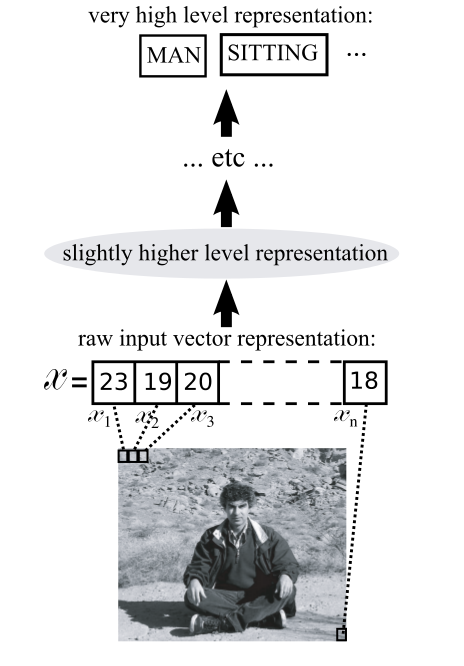
\includegraphics[width=3.5in]{Images/Introduction/DL_principle.png}
				\caption{Deep learning procedure applied to a computer vision example}
				\label{fig:Example of deep architecture for a computer vision}
			\end{center}
		\end{figure}
  
		Thus, deep learning methods aim at automatically  and recursively learn higher level feature hierarchies among features themselves composed of lower level features. By doing so, we allow the system to learn complex functions mapping ``directly'' the raw data to the output, \Important{without relying on any hand-crafted features.}\\\par 
  
  
		\section{Outline of the report:}
		\label{seq:Introduction/Outline of the report}    
		The aim of this report will be to provide a broad overview on deep neural networks and on the observations realized during my internship. We will start by introducing the concepts required to understand what an artificial neural network is (chapter~\ref{chap:Artificial neural networks}). We will describe the mathematical concepts it is constructed upon, how it is trained and provides several successful examples of applications.\\\par
		
		Second, we will focus on the deep neural networks themselves (chapter~\ref{chap:Deep neural networks}). We will define more precisely the notion of depth and how it is measured, then explain what the advantages of deep architectures are. We will give an overview of the bottlenecks that have limited the use of deep neural networks before and describe a training procedure adapted to those architectures. Finally we will have a look at how those networks are built.\\\par
				
		In a third and fourth chapters, two types of deep neural network will be introduced in more details. First the the deep belief network -chapter~\ref{chap:DBN:}- and then the stack auto-encoders -chapter~\ref{chap:AE and SAE:}. We will describe the theoretical background of those networks as well as their training procedure.
		
		In a fifth chapter, we will have a look to how the over-fitting risk is managed for the auto-encoders. Indeed, due to their learning procedure those networks are very likely to over-fit to the training data and several methods exist to prevent this. We will provide there an overview of those regularization methods (chapter~\ref{chap:Regularization methods for Auto-encoders}).\\\par
		
		The sixth chapter will be dedicated to the description of the technical choices made during the internship to implement the stack auto-encoders (chapter~\ref{chap:Implementation of the SAE:}). We will have a look at the Python library used to leverage the GPUs for training the deep neural networks and then present the implemented objects.\\\par
		
		The final chapter will offer an overview of the experiments run using the deep machines implemented during the internship (chapter~\ref{chap:Experimental results}). We will first assess the performances on the famous MNIST dataset \cite{LeCun_webPage} and then present the results obtained on an unknown data analysis problem.\\\par
		
%%%%%%%%%%%%%%%%%%%%%%%%%%%%%%%%%%%%%%%%%%%%%%%%%%%%%%%%%%%%%%%%%%%%%%%%%%%%%%%%%%%%%%%%%%%%%%%%%%%%%%%%%%%%%%%%%%%%%%%%%%%%%%%%%%%%%%%%%%%%%%%%%%%%
\chapter{Scattering transform:}
	\label{chap:Scattering transform}
	In this section, basic and general information will be provided about the artificial neural network in order to set the basis of the concepts necessary to study artificial deep neural networks.\\\par
 
	When one refers to an -artificial- neural network, one usually narrows the concept down to the feedforward neural networks. This is one of the most basic types of artificial neural networks designed to learn distributed representations of the input data. It consists of a \Important{series of information processing operations}, whereby information moves strictly in a forward direction (i.e.: no retro-action loop), from the input units, through latent -hidden- units, if any and finally to the output units. 

	
	\section{Convolutional Neural Network:}
		\label{seq:Artificial neural networks/Perceptron network}
		The simplest form of feedforward neural network is the perceptron \cite{Rosenblatt_1958}, built using the mathematical model of a formal neuron \cite{McCulloch_1943}. \\\par
    
		\begin{figure}[H]
			\begin{center}
				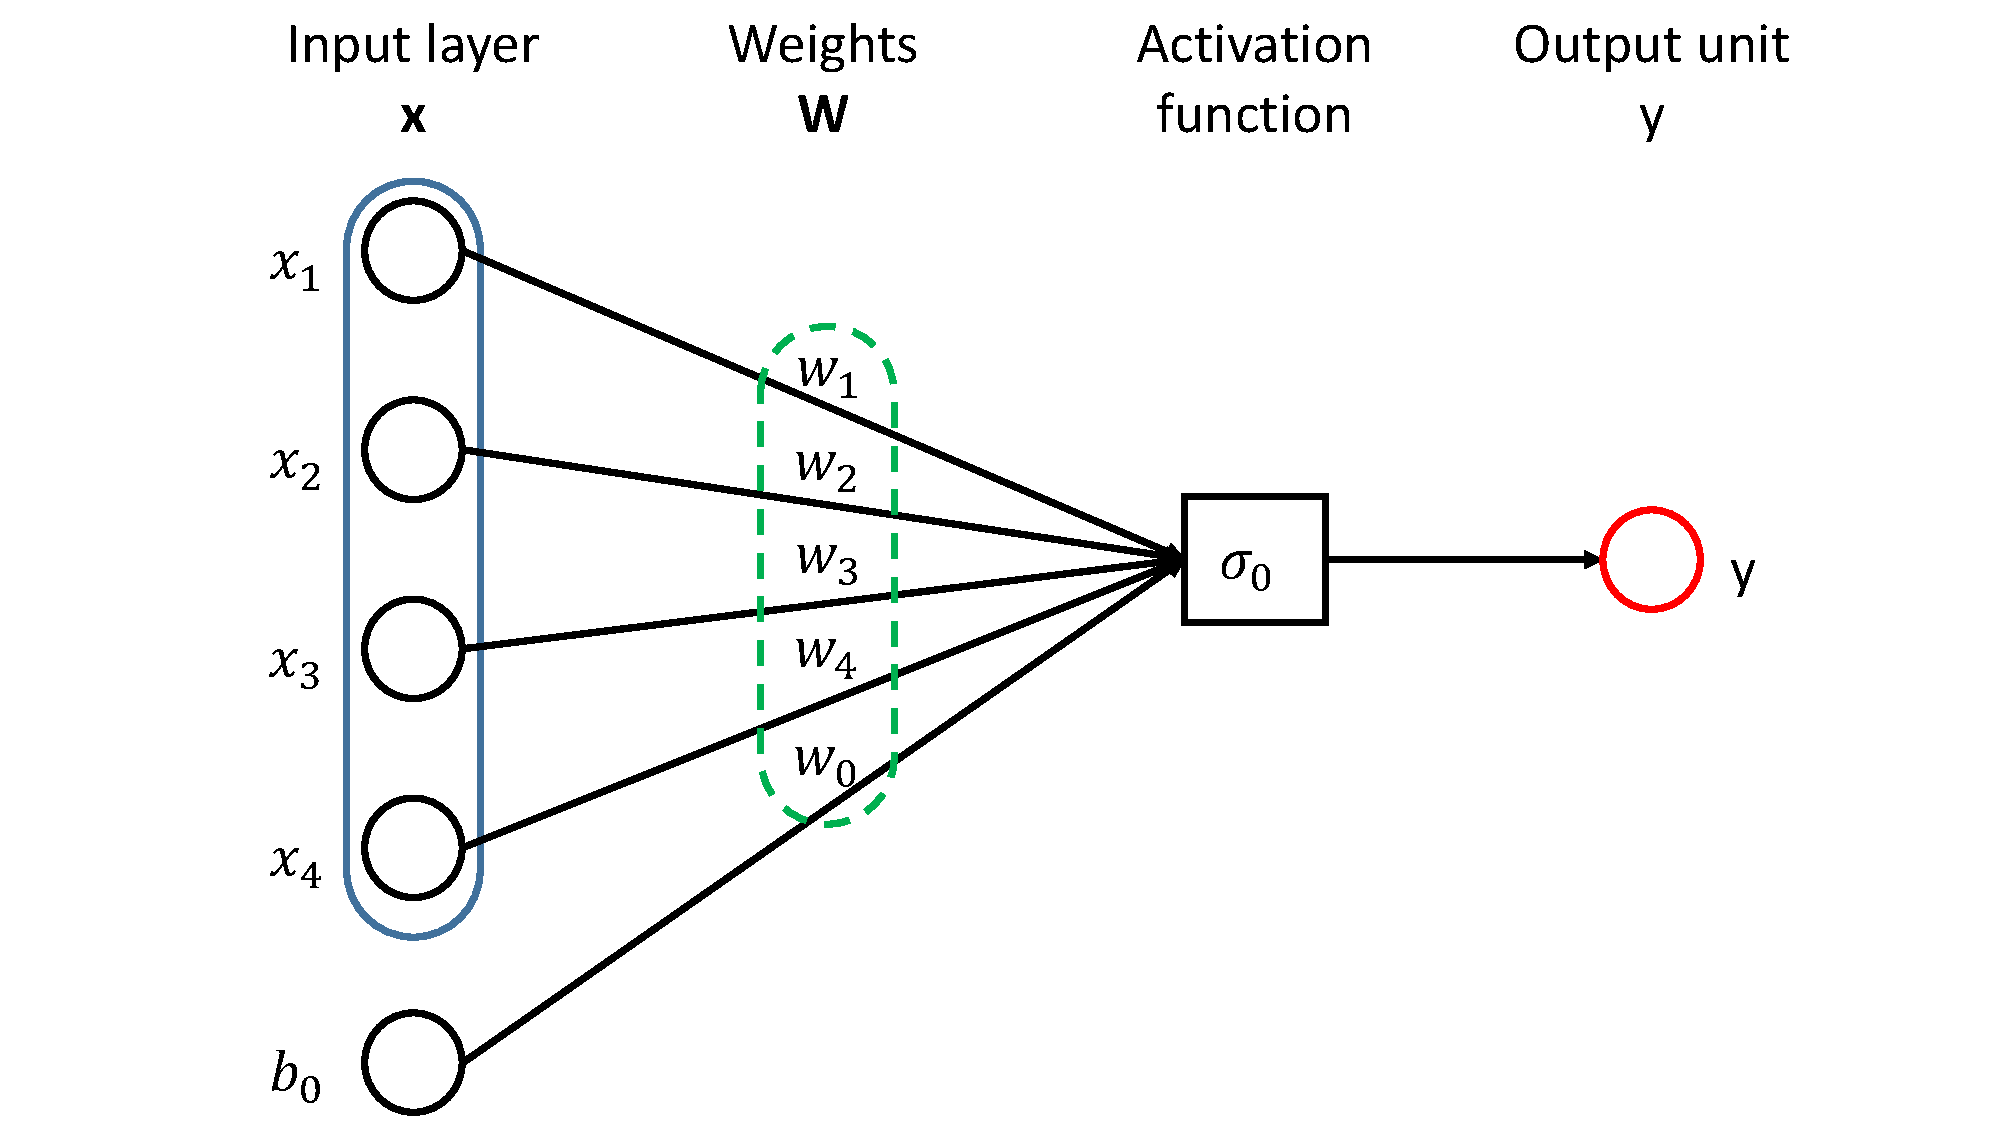
\includegraphics[width=2.5in]{Images/NN/perceptron_network.pdf}
				\caption[The perceptron network]{The perceptron network: Uses a set of weights $\mathbf{W}$ and a feedforward activation function $\sigma_{0}$ to map a layer of input units $\mathbf{x}$ to the output unit $\mathbf{\hat{y}}$}
				\label{fig:The perceptron network}
			\end{center}
		\end{figure}
    
		As illustrated in Figure~\ref{fig:The perceptron network}, the output value $\mathbf{\hat{y}}$ of an input vector $\mathbf{x}$ is obtained from a set of weights -parameters- $\mathbf{W}$ and a feedforward activation function $\sigma_{0}$. The coefficient $w_{0}$ is a parameters known as the bias -or offset- and it is connected to an input unit $b_{0}$ that is permanently set to 1. For an input with $N$ dimensions, the mathematical expression of the output may be:\\
		
    \begin{itemize}
      \item \Important{Linearly activated:} through a weighted sum of the inputs.
      \begin{equation}
        \mathbf{\hat{y}} = \sigma_{0}(\mathbf{x},\mathbf{W}) = \sum_{i=0}^{N} w_{i} x_{i}        
      \end{equation}\\
			
			\item \Important{Binarized:} by a threshold $t$.
			\begin{equation}
				\mathbf{\hat{y}} = \sigma_{0}(\mathbf{x},\mathbf{W}) = 
				\begin{cases}
					1 & \text{if } \sum_{i=0}^{N} w_{i} x_{i} \geq t \\
					0 & \text{otherwise}
				\end{cases}
			\end{equation}\\
		\end{itemize}     
     
			Depending on the application and the objective of the learning (discrimination, generalization...), many different activation functions $\sigma_{0}$ can be used. The list bellow is far from exhaustive but introduces the most common ones:\\
			
			\begin{itemize}
				\item \Important{The step function:} This is the function historically used by the first perceptron model. It has the advantage of offering very straight forward computation. However with the progress done in the domain of computational power, some more complex functions are usually preferred over this one.\\
				\begin{equation}
					\mathbf{\hat{y}} = \sigma_{0}(\mathbf{x}, \mathbf{W}) =         
					\begin{cases}
						1  & \text{if } \sum_{i=0}^{N} w_{i} x_{i} \geq 0 \\
						0 & \text{otherwise}
					\end{cases} 
				\end{equation}
				\begin{figure}[H]
					\begin{center}
						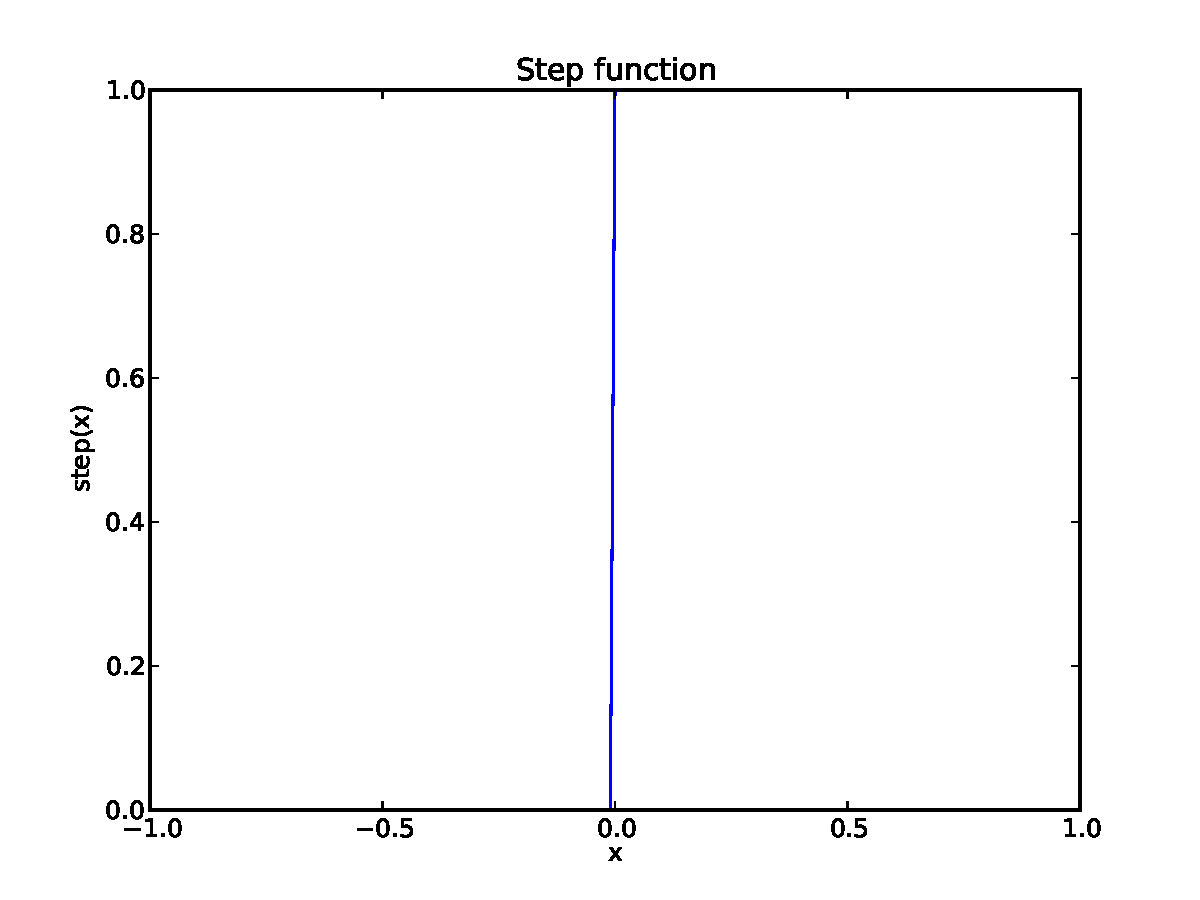
\includegraphics[width=3 in]{Images/NN/step.pdf}
						\caption[Activation function: The step function]{The step function: Historically used in the first model of artificial network}
						\label{fig:The step function}
					\end{center}
				\end{figure}
       
				\item \Important{The sigmoid function:} It is the most popular activation function mainly because its derivatives are easy to compute \footnote{For the sigmoid function $f$: $f' = f(1 - f)$}. It can be used for binary classification problems as well as regression ones.\\
				\begin{equation}
					\mathbf{\hat{y}} = \sigma_{0}(\mathbf{x},\mathbf{W}) = \frac{1}{1 + \exp{(-\sum_{i=0}^{N} w_{i} x_{i}})}
				\end{equation}
				\begin{figure}[H]
					\begin{center}
						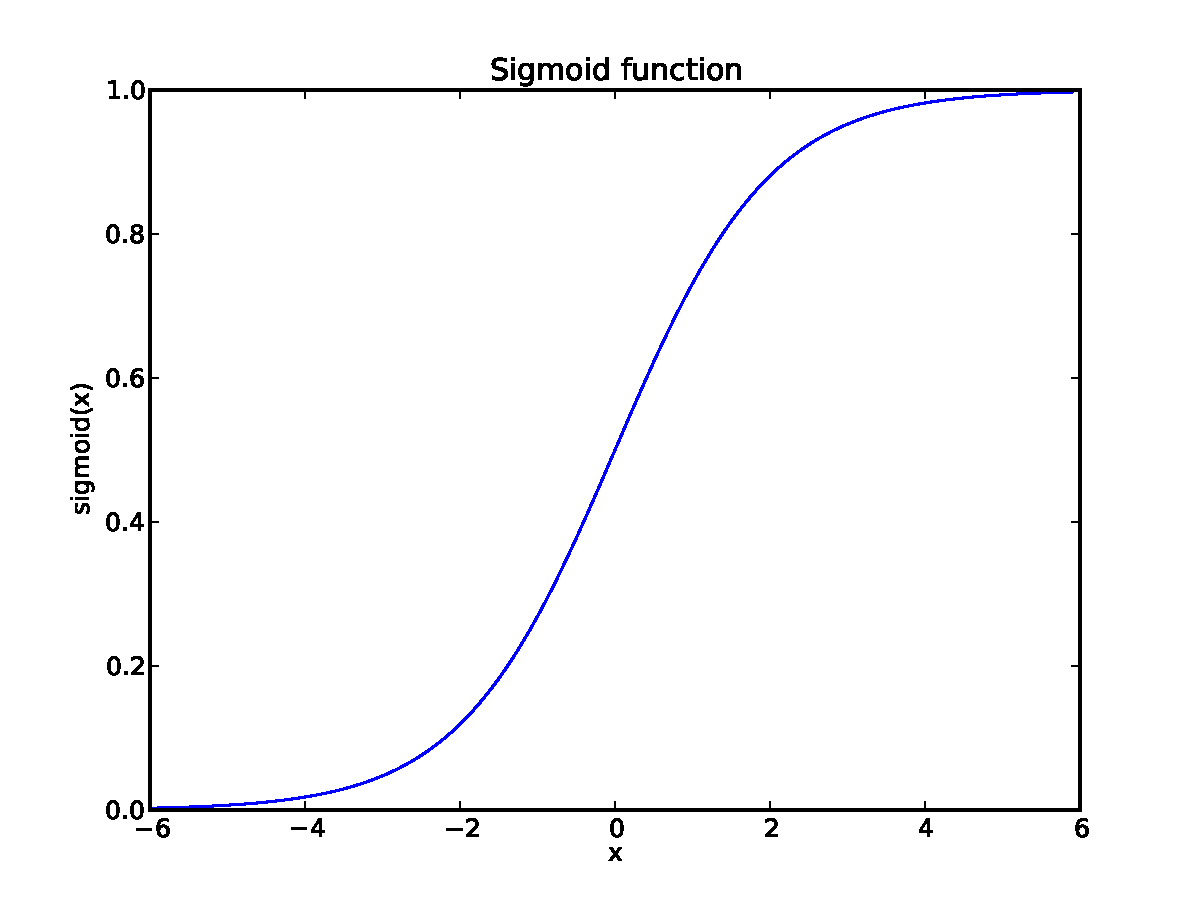
\includegraphics[width=3 in]{Images/NN/sigmoid.pdf}
						\caption[Activation function: The sigmoid]{The sigmoid function: The most widely used activation function for binary classification and regression problems}
						\label{fig:The sigmoid function}
					\end{center}
				\end{figure}    
       
				\item \Important{The hyperbolic tangent function:} This activation function is also quite popular for binary classification or regression problems and its derivatives are also quite easy to compute \footnote{For the hyperbolic tangent function $f$: $f'= 1 - f^{2}$}. It can be used on the same type of problem as the sigmoid but offers a stronger discriminative capacities (because of steeper derivatives in the middle of the domains) than the sigmoid which can be an advantage in some situations.\\
				\begin{equation}
					\mathbf{\hat{y}} = \sigma_{0}(\mathbf{x}, \mathbf{W}) = \tanh\left(\sum_{i=0}^{N} w_{i} x_{i}\right)
				\end{equation}
				\begin{figure}[H]
					\begin{center}
						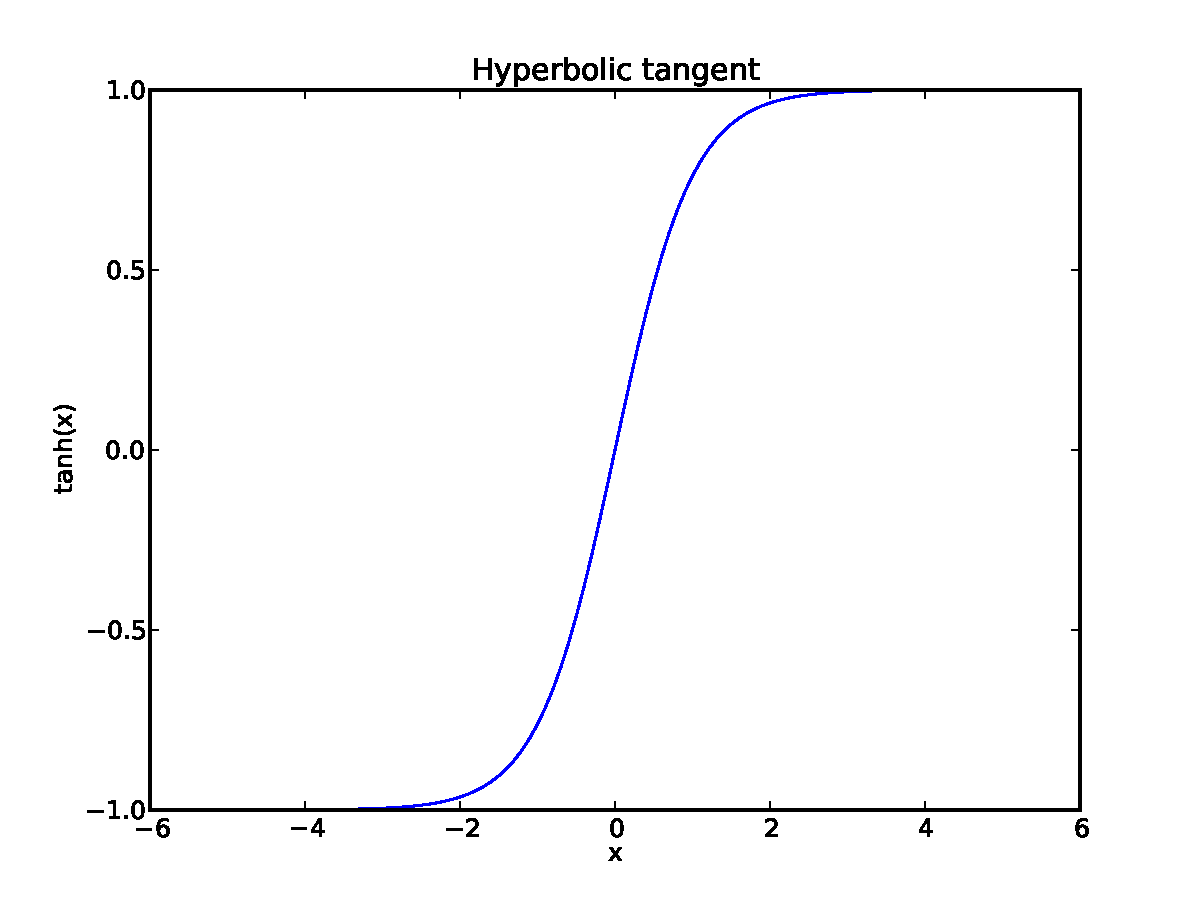
\includegraphics[width=3 in]{Images/NN/tanh.pdf}
						\caption[Activation function: The hyperbolic tangent]{The hyperbolic tangent function: Another widely used activation function for binary classification problems as well as regression ones}
						\label{fig:The hyperbolic tangent function}
					\end{center}
				\end{figure}  
       
				\item \Important{The rectified linear function:} This activation function has been highlighted recently as it seems to provide, in some cases, better results than the classic sigmoid for deep neural networks. Again this is due to a higher discriminative performances helpful in some cases.\\
				\begin{equation}
					\begin{split}
						\mathbf{\hat{y}} = \sigma_{0}(\mathbf{x}, \mathbf{W}) =         
						\begin{cases}
							\alpha\sum_{i=0}^{N} w_{i} x_{i}  & \text{if } \sum_{i=0}^{N} w_{i} x_{i} \geq 0 \\
							0 & \text{otherwise}
						\end{cases} \\
						= \max(0, \sum_{i=0}^{N} w_{i} x_{i})
					\end{split}
				\end{equation}
				\begin{figure}[H]
					\begin{center}
						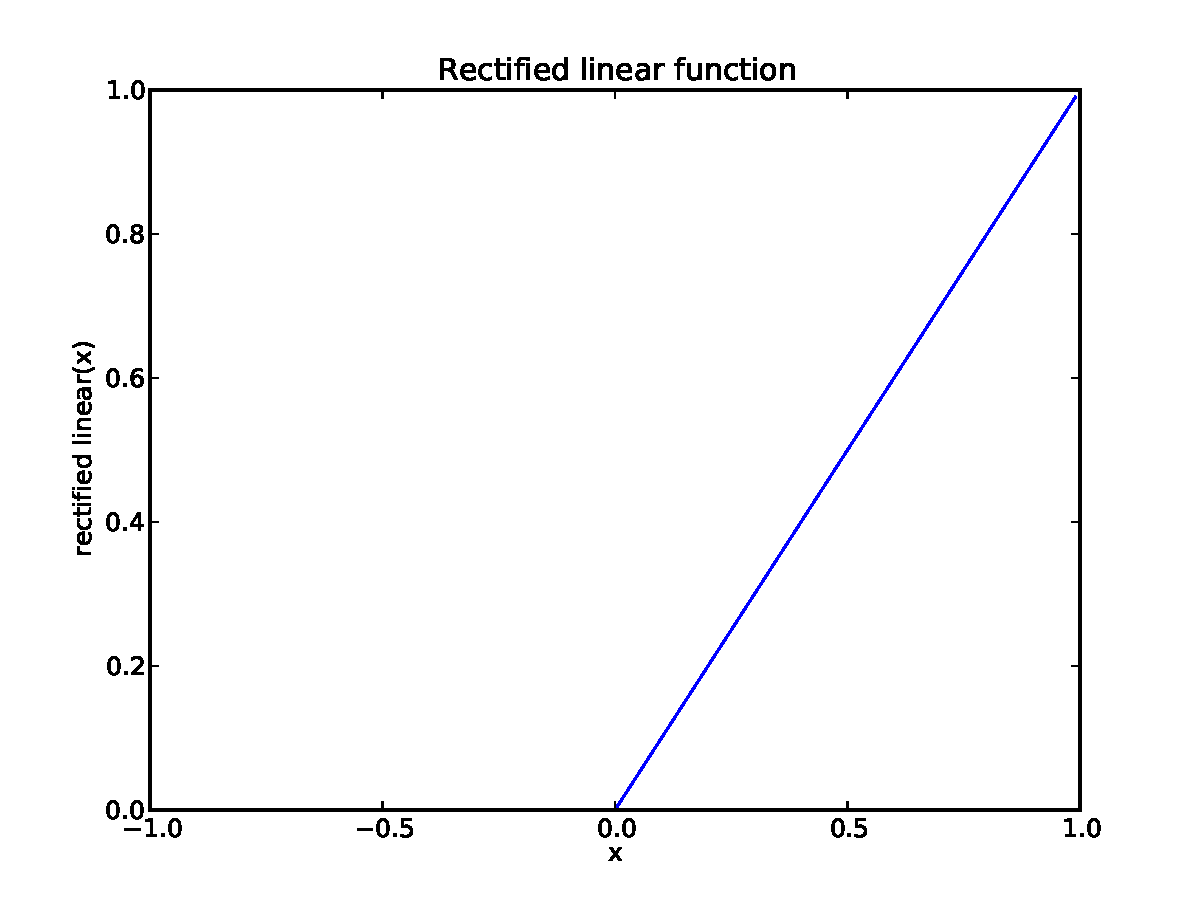
\includegraphics[width=3 in]{Images/NN/rl.pdf}
						\caption[Activation function: The rectified linear]{The rectified linear function: A fairly new activation function for binary classification problems that seems to have better discrimination capacities compared to the sigmoid function}
						\label{fig:The rectified linear function}
					\end{center}
				\end{figure}
       
				\item \Important{The softmax function:} This activation function is the multi-classes version of a sigmoid. It is useful predominantly in the output layer of a clustering system.
				\begin{equation}
					\mathbf{\hat{y}}_{j} = f_{e}(\mathbf{x}, \mathbf{W})_{j} = \frac{\exp(w_{j}x_{j})}{\sum_{i=0}^{N} \exp(w_{i} x_{i})}
				\end{equation}\\     
			\end{itemize}
 
 
	\section{Scattering network:}
		\label{seq:Artificial neural networks/The cost function}
		The cost function is used to measure the error done by the learned predictor. It has to measure the difference between an the prediction $\hat{y}$ done by the predictor for an example $\mathbf{x}$ and the effective label of the input $y$. A cost function should tends to $0$ when $\hat{y} \rightarrow y$.\\\par
		
		While, the cost function used in the training procedure (section~\ref{seq:Artificial neural networks/Training by error backpropagation} and the equation~\ref{eq:gradient descent updates}) can be tailored to the problem tackled (custom made cost function leveraging specific prior knowledge on the dataset to be learned), there are also several usual error functions.
    
		\subsection{0-1 loss:}
			This is the simplest error function. It is not widely used anymore as it is too simple to allow good learning performances as well as because it does not have interesting derivatives.
			
			\begin{equation}
				J(x,y) =
				\begin{cases}
					0 & \text{if } x = y \\
					1 & \text{if } x \neq 0
				\end{cases}
			\end{equation}\\

      
		\subsection{Squared loss:}
			This is an error function based on the $L_{2}$ norm. It is one of the most generic lost function and it can be used for the classification or regression problems whenever there is no special metric tailored o the problem.
			
			\begin{equation}
				J(x,y) = \|y-x\|_{2}
				\label{eq:squared}
			\end{equation}\\
			
		\subsection{Cross-entropy loss:}
			This metric is mostly used with stochastic machines (such as the RBMs - chapter~\ref{chap:DBN:}) or when the inputs are interpreted as \Important{bit vectors  or as vectors of bit probabilities}. Its general expression is:
			
			\begin{equation}
				J(x,y) = - x \log y + (1 - x)\log(1 - y)
				\label{eq:Cross-entropy}
			\end{equation}\\
          
	\section{Spatial Wavelet transform:}
		\label{seq:Artificial neural networks/Multilayer perceptron network}
		
		A \Important{Multilayer Perceptron network} (MLP) consists of multiple stacked perceptron where each layer is fully connected to the next one but where there is no intra-layer connection. Figure~\ref{fig:The multi-layers perceptron network} presents a three-layer MLP. The first layer is a passive (i.e.: no computation done) input layer, followed by an hidden (i.e.: latent) layer where a first level of representation of the data is computed. Finally, the third and output layer performs the computation of a second level of representation of the input data. 
		
		\begin{figure}[H]
			\begin{center}
				\caption[A Multi-layers perceptron network]{Three-layer multi-layer perceptron: Use two successive steps of weighted data information processing (latent layer and output layer) to map the  inputs to the outputs}
				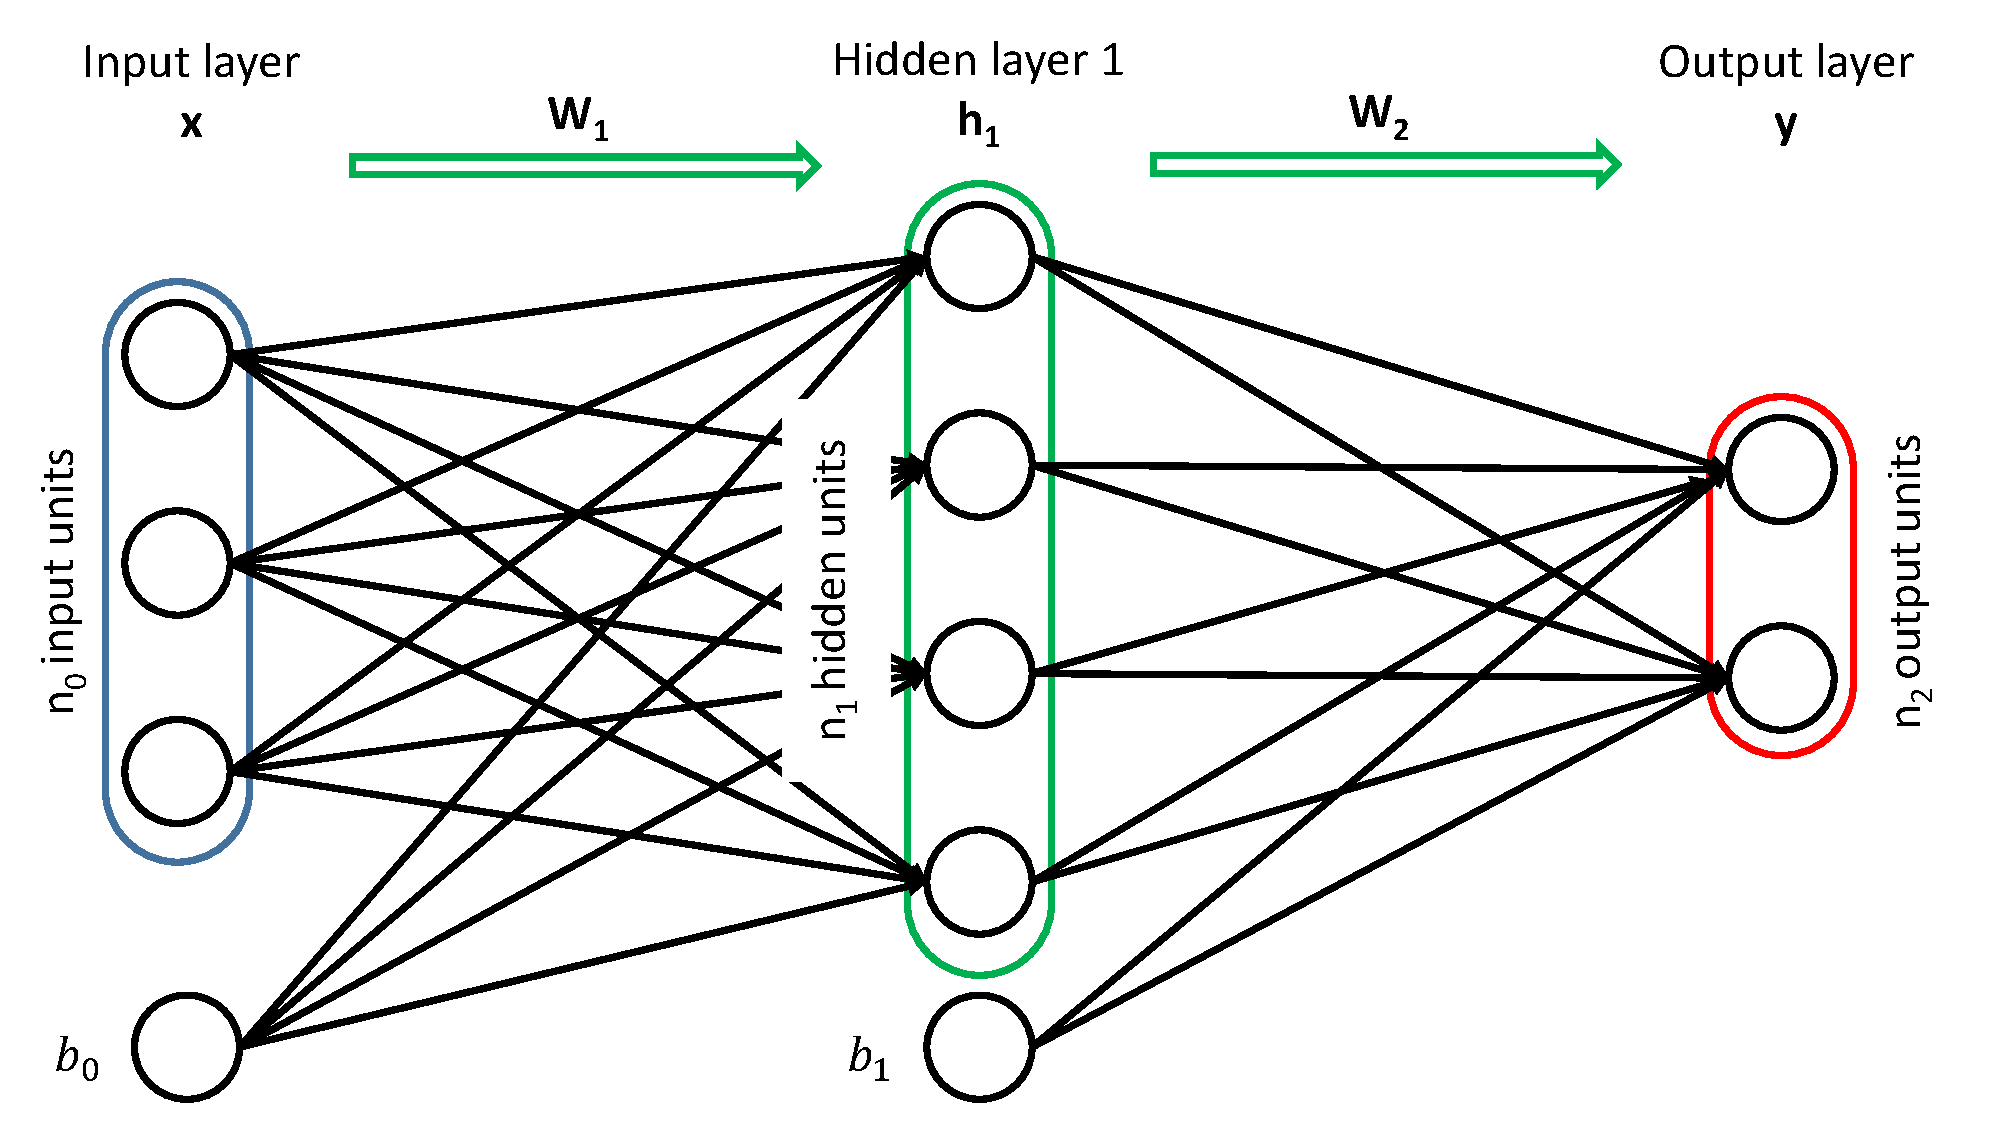
\includegraphics[width=2.5in]{Images/NN/MLP.pdf}
				\label{fig:The multi-layers perceptron network}
			\end{center}
		\end{figure}
       
		Unlike the perceptron network, the multi-layer perceptron is able to learn a model of data that is not linearly separable. A \Important{three-layer MLP is considered to be a universal approximator of continuous functions}. This was proven by \cite{Cybenko_1989} for sigmoid activation function and by \cite{Hornik_1991} for the multi-layer feedforward network in general, regardless of the choice of activation function
		
		
	\section{Roto-translation wavelet transform:}
		\label{seq:Artificial neural networks/Training by error backpropagation}
			
		A multi-layer perceptron is trained using the combination of two algorithms:\\
		\begin{itemize}
			\item \Important{The Backpropagation algorithm:} To compute the partial derivatives of the cost function used with regard to each parameters of the network \cite{LeCun_1985,Rumelhart_1986}.\\
			\item \Important{The Gradient descent algorithm:} To find the optimal parameters that minimize the cost function over the training set.\\
		\end{itemize}
 		
 		Let us consider a labeled training set $\mathcal{D}_{train} = (\mathbf{x_{k}},y_{k})_{k \in [0, |\mathcal{D}_{train}|]}$ used to train a d-layers perceptron and let us define the following notations:\\
 		
 		\begin{itemize}
			\item $J(\mathbf{W},\mathbf{b},\mathbf{x_{k}},y_{k})= J(\mathbf{x_{k}},y_{k})$: the cost function associated to an example $x_{k}$ and to the network parameters $\mathbf{W}$ and $\mathbf{b}$.\\
			
			\item $z^{(l+1)} = W^{(l)} x_{k} + b^{(l)}$: The input of the layer $l+1$.\\
			
			\item $a^{(l+1)} = \sigma_{k}(z^{(l+1)}$:The value of the activation of the layer $l$.\\ 
 		\end{itemize}

 		The backpropagation procedure for a given tuple of training examples $(\mathbf{x}_{k},y_{k})$  is described by the algorithm~\ref{algo:backpropagation}:\\
		
		\begin{center}
			\begin{algorithm}[H]
				1) Perform a feedforward pass, computing for each $k \in [1, d-1]$, the activation $a^{k}$ for the layer $L_{k}$.\\
				2) For the output layer $L^{(d)}$ set: \\
				\begin{equation}
					\delta^{(d)} = \frac{\partial }{\partial \mathbf{z^{(l)}}} J(\mathbf{x_{k}},y_{k})
					\label{eq:last layer error for backpropagation}
				\end{equation}\\
				3)\For{ l in [d-1,...,1]}{
					Set:
					\begin{equation}
						\delta^{(l)} = (\mathbf{W^{(l)}})^{T} \delta^{(l+1)}
					\end{equation}\\
					}
				4) Compute the desired partial derivatives:
					\begin{subequations}
						\label{eq:backpropagation}
						\begin{align}
							\nabla_{W^{(l)}} J(\mathbf{W},\mathbf{b},\mathbf{x_{k}},y_{k}) & = \delta^{(l+1)}(a^{(l)})^{T} \\
							\nabla_{b^{(l)}} J(\mathbf{W},\mathbf{b},\mathbf{x_{k}},y_{k}) & = \delta^{(l+1)}
						\end{align}
					\end{subequations}
				\caption{The backpropagation algorithm on a d-layer perceptron}
				\label{algo:backpropagation}		
			\end{algorithm}        
		\end{center}
		
		And then the error backpropagation is used to train a multi-layer perceptron with continuous differentiable activation functions and it can be described as follow:\\
		
		\begin{center}
			\begin{algorithm}[H]
				1) Set $\Delta \mathbf{W}^{(l)} := 0$, $\Delta \mathbf{b}^{(l)} := 0$ (matrix/vectors of zeros for all layers $l$).\\
				2) \For{$k= 1 \text{to} |\mathcal{D}_{train}|$}{
							2.a) Use the backpropagation algorithm~\ref{algo:backpropagation} to compute $\nabla_{W^{(l)}} J(\mathbf{W},\mathbf{b},\mathbf{x_{k}},y_{k})$ and $\nabla_{b^{(l)}} J(\mathbf{W},\mathbf{b},\mathbf{x_{k}},y_{k})$\\
							2.b) Set: $\Delta \mathbf{W}^{(l)} := \Delta \mathbf{W}^{(l)} + \nabla_{W^{(l)}} J(\mathbf{W},\mathbf{b},\mathbf{x_{k}},y_{k})$\\
							2.c) Set: $\Delta \mathbf{b}^{(l)} := \Delta \mathbf{b}^{(l)} + \nabla_{b^{(l)}} J(\mathbf{W},\mathbf{b},\mathbf{x_{k}},y_{k})$
						}
				3) Update the parameters:
					\begin{subequations}
						\label{eq:gradient descent updates}
						\begin{align}
							\mathbf{W}^{(l)} &:= \mathbf{W}^{(l)} - \alpha \frac{\Delta \mathbf{W}^{(l)}}{m}\\
							\mathbf{b}^{(l)} &:= \mathbf{b}^{(l)} - \alpha \frac{\Delta \mathbf{b}^{(l)}}{m}
						\end{align}
					\end{subequations}
				\caption[A simple gradient descent algorithm]{A simple gradient descent algorithm for a learning rate $\alpha$}
				\label{algo:Gradient descent algorithm}		
			\end{algorithm}        
		\end{center}
    
		Note that those algorithms requires to use activation functions with defined derivatives and that some activation functions introduced in the previous section (section~\ref{seq:Artificial neural networks/Perceptron network}) are not differentiable (step function, rectified linear function...) over $\mathbb{R}$. However most of the time, the derivatives of the activation function can easily be extended over all $\mathbb{R}$.\\\par
   
		Note also that the procedures given here describe the simplest gradient descent algorithm but several improvements have been proposed to improve its accuracy. Among those improvements, there is the mini-batch gradient descent \cite{Ng_course}, which average the update to be made over several training examples. This method speed up the convergence toward the optimal parameters by minimizing the effect of outliers on the descent. Another first order variation of the gradient descent widely used to train -deep- neural networks is the stochastic gradient descent but some researchers start to recommend to use second order optimization methods -such as L-BFGS- to train the neural networks \cite{Ng_course, Bengio_2009}.\\\par
		
		As an example for the calculation, let us applied those algorithms to a three layers MLP (Figure~\ref{fig:The multi-layers perceptron network}), with an input layer $\mathbf{x} \in \mathbb{R}^{I}$ mapped to a latent layer $\mathbf{h} \in \mathbb{R}^{J}$ via the weights matrix $\mathbf{W_{1}}$, itself mapped to an output layer $\mathbf{\hat{y}} \in \mathbb{R}^{C}$ via the weight matrix $\mathbf{W_{2}}$. Suppose that we are using a loss function $\mathcal{L}$ -either a tailored one or one described in the section~\ref{seq:Artificial neural networks/The cost function}- then the weights of the network can be updated using the following procedures:
		
		\begin{equation}
			\begin{split}
				w_{2,j,c} &= w_{2,j,c} + \epsilon \frac{\partial \mathcal{L}}{\partial w_{2,j,c}} \\
				w_{1,i,j} &= w_{1,i,j} + \epsilon \frac{\partial \mathcal{L}}{\partial z_{j}} \frac{\partial z_{j}}{\partial w_{1,i,j}}
			\end{split}
		\end{equation}
    
    
	\section{Application to classification:}
		\label{seq:Artificial neural networks/Applications and Limits}
		Artificial neural networks can be used on a wild range of applications. As seen in section~\ref{seq:Artificial neural networks/Multilayer perceptron network}, neural networks are universal approximators. Thus they are theoretically able to learn any kind of relationship in between the input and the output. As we will see in section~\ref{seq:Deep neural networks/Depth definition}, these results are only theoretical and the performances of classical multi-layers perceptron are limited, however they perform very well for tasks such as capturing associations or discovering regularities within a set of patterns, applications where the volume, the number of variables or diversity of the data is very great (compared to SVMs for example), applications where the relationships between variables are vaguely understood or, application where the relationships are difficult to describe adequately with conventional approaches. \\\par
    
		For example, they have been successfully applied for classification problem, such as hand-written digit recognition \cite{LeCun_webPage}, or for regression problems, such as predict the credit score of a individual \cite{West_2000}.
    
%%%%%%%%%%%%%%%%%%%%%%%%%%%%%%%%%%%%%%%%%%%%%%%%%%%%%%%%%%%%%%%%%%%%%%%%%%%%%%%%%%%%%%%%%%%%%%%%%%%%%%%%%%%%%%%%%%%%%%%%%%%%%%%%%%%%%%%%%%%%%%%%%%%%
\chapter{Probabilistic graphical models:}
	\label{chap:Deep neural networks}
	In this chapter, we will introduce the concept of deep neural networks more at length by first defining the notion of depth. Once this question solved, we will assess the various motivations to make such important push toward this type of networks. We will then explain the specific training procedure used for deep networks and finally describe the main types of deep neural networks.

	
	\section{Bayesian Network:}  
		\label{seq:Deep neural networks/Depth definition}
		Formally the \Important{depth is not a intrinsic property of an architecture}. It depends on the \Important{set of computational elements} (i.e.: the family of ``operators'') considered. Thus, given a set of computational elements, one can define the depth of an architecture as the depth of the graph involved to compute the output from the input. Formally it is the longest path from an input node to an output node.
               
		\begin{figure}[H]
			\begin{center}
				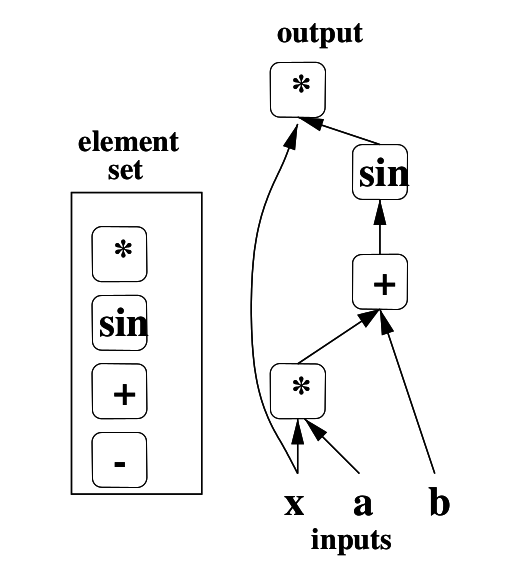
\includegraphics[width=2.5in]{Images/DNN/depth_example.png}
				\caption[The computation of depth]{Computation of the depth for $f(x)= x.sin(a.x +b)$ for the set of computational elements $(x, +, -, sin)$}
				\label{fig:Computation of the depth}
			\end{center}
		\end{figure}
        
		For example, let us assess the depth of the representation of the function $f(x)= x.sin(a.x + b)$ given the set of computational elements $(x, +, -, sin)$. The graph of this computation is illustrated in Figure~\ref{fig:Computation of the depth} and it has a depth of $4$. Because the multiplication $a.x$ and the final multiplication by $x$ are computed by two different layers.\\\par
    
		For the most classic machine learning applications we have the following depth:\\
		\begin{itemize}
			\item \Important{Linear or logistic regression} have a depth equal to 1 if the set of computational elements includes affine operations as well as their possible compositions with sigmoids.\\
			
			\item \Important{Kernel machines} have a depth of 2 if we include a fixed kernel computation $K(\mathbf{u},\mathbf{v})$ in the family of ``operators''. The first level has a single element performing the computation of $K(\mathbf{x_{i}},\mathbf{c})$ for each training example $\mathbf{x_{i}}$ and matches the training example $\mathbf{x_{i}}$ with the input vector $\mathbf{x}$. Then the second level realizes an affine combination $b+\sum_{i}{\alpha_{i} K(\mathbf{x},\mathbf{x_{i}})}$ to compute the expected output for an example $\mathbf{x_{i}}$.\\
			
			\item For \Important{Neural networks}, the \Important{depth is equal to the number of layers} (excluded the input layer as it does not perform any computation) if we define the set of computational elements as the set of computations an artificial can neuron perform. For example a one hidden layer neural network will have, for this set of computational elements, a depth of 2 (the hidden and the output layer).\\
			
			\item \Important{Decision trees} can be seen as having a depth of 2 (see \cite{Bengio_2009} for explanations).\\
			
			\item \Important{Boosting} adds one level of deepness to the base learner used \cite{Freund_1996}.\\
		\end{itemize}
       
		As a comparison, according to the current research on brain anatomy \cite{Serre_2007}, the visual cortex itself could be seen as a deep architecture of 5 to 10 levels.\\\par
        
		So far, we have define depth as an extrinsic parameters of the learner conditioned by how we define the set of computational elements. But a graph associated with one set can, most of the time, be converted to the graph associated to another set by graph transformation in a way that multiplies the depth. Moreover, theoretical results suggests that \Important{it is not the absolute value of the depth that matters} but the \Important{relative depth} compared to the depth of a efficient representation of the approximated function with this set of computational elements.
     
     
	\section{Hidden Markov Models:}
		\label{seq:Deep neural networks/Advantages of a deep architecture}  
		The advantages of deep architecture are of various natures. One can advocate in favor of a deep architecture using computational, statistical or even biological arguments.
            
		\subsection{Computational advantages:}
			\label{subseq:Deep neural networks/Advantages of a deep architecture/Computational advantages}      
			The expression of a function given by a machine learning algorithm is said \Important{compact} when it has only a few degrees of freedom to be  tuned by learning (i.e.: a few computational elements). A compact representation of a function will be expected to yield to better generalization than a loose representation for a fixed number of training example. Indeed, the compact expression will have less parameters to be tuned during the learning phase and so is expected to reach a point in the optimization space closer to the actual optimum. \\\par
    
			Thus the main idea used to defend deep architecture is that \Important{some function are simply too complicated to be compactly represented by a too shallow architecture}. In section~\ref{seq:Artificial neural networks/Multilayer perceptron network} we have seen that a neural network of depth 2 (i.e.: with one hidden layer) is an universal approximator. Thus a network of this depth will be theoretically sufficient in most of the cases (e.g.: logical gates, sigmoid-neurons, Radial Basis Function 'RBF' units like in SVMs) to reach a targeted accuracy on a given problem. Having said this, the number of neurons required to perform the representation may be very large and we are very likely to obtain a loose representation of the objective function. Indeed some theoretical results for logical gates, formal neurons and RBF units have shown that, in the worst case scenario (i.e.: for specific function families) the required number of nodes to realize the compact representation may grow exponentially with the 
dimension of the input. For the RBF units, Hastad has even described families 
of functions which can be compactly represented with a linear number of nodes $O(n)$ for an input of dimension $n$ and a network of depth $d$ but required an exponential size $O(2^{n})$ for the same input if the network is of a depth $d-1$ \cite{Hastad_1986}.\\\par
      
			Those results are only proved for a specific family of function and does not proved that the functions to be learned in machine learning fall into this category. They also apply only to a specific kind of circuit and there is no proof for a generalized version of this property. Despite those gaps, this property is often use to advocate in favor of deep architecture \cite{Bengio_2009, Ng_course}, as increasing the number of layers is expected to reduce the complexity of our network (i.e.: reduce the number of parameters to be handled) and thus decreasing the computational performances required.
      
		\subsection{Statistical advantages:}
			\label{subseq:Deep neural networks/Advantages of a deep architecture/Statistical advantages}      
			Using the same abusive generalization of the property demonstrated by Hastad for the RBF, one can also advocate in favor of a deep architecture using a statistical argument. Indeed, since the number of parameters that can be tuned/selected during the learning phase depends on the number of training examples available, the use of a loose representation of the objective function, with more free parameters, may lead to a poorer learning quality compared to a learning done on a compact representation on the same number of training examples. Thus a loose representation is expected to lead to poor generalization capacities.\\\par
     
			One can see a deep architecture as a kind of factorization of the problem. A completely random function cannot be represented efficiently, whether with a deep or a shallow architecture. But when there is a logic to be learned, many that can be represented efficiently with a deep architecture cannot be represented efficiently with a shallow one (see the polynomials example in \cite{Bengio_2009}). The existence of a compact and deep representation indicates that some kind of structure exists in the underlying function to be represented. If there was no structure whatsoever, it would not be possible to generalize well.
    
		\subsection{Biological advantages:}
			\label{subseq:Deep neural networks/Advantages of a deep architecture/Biological advantages}
			
			One of the goal in machine learning is to allow computers to model our world well enough to exhibit what is called ``intelligence''. Many scientists are convinced that this can be achieved only by recreating a brain-like architecture for machine learning procedures. In that sense, deep networks seems very adapted as most of the brain scientists agree to say that the brain works using several successive layers of representation to process the information.\\\par
			
			For example, the well-studied visual cortex shows a sequence of areas each of which contains a representation of the input, and signal flow from one to the next. There are also skip connections (a kind of natural dropout - see section~\ref{seq:Regularization methods for Auto-encoders/Dropout:}) and at some level parallel paths, so the procedure is still way more complex than what is currently done with deep networks. But the main idea remains. At each level of this feature hierarchy, a representation of the input at a different level of abstraction is created with more abstract features further up in the hierarchy, defined in terms of the lower-level ones.\\\par
      
			Brain researchers have also noticed that representations in the brain are not dense, neither purely local. They are \Important{sparse}. For a given task, \Important{about $1\%$ of neurons are active  simultaneously in the brain}. Given the huge number of neurons, this is still a very efficient (exponentially efficient) representation. This observation can be use to advocate in favor of deep architecture with a sparse regularization (see section~\ref{seq:Regularization methods for Auto-encoders/Sparsity:}) to mimic the brain behavior.\\\par
      
			Finally the cognitive processes themselves seem deep. Indeed, humans organize their ideas and concepts hierarchically.They first learn simpler concepts and then compose them to represent more abstract ones. For example an engineer facing a problem will break-up the solutions into multiple sub-problems and sub-solutions (i.e.: multiple levels of abstraction and processing). And this is what an ideal deep architecture would do facing a problem.
    
    
% 	\section{The training procedure:}
% 		\label{seq:Deep neural networks/The training procedure}
% 		With those consistent evidences toward the utility of deep architecture, it is surprising that their usage only emerged recently. The reason for their late fame is that prior to 2006 and the work of Geoffrey Hinton, there was no efficient method to train deep neural network and they usually lead to worst generalization performances than shallow networks. Indeed we will seen in the section~\ref{subseq:Deep neural networks/The training procedure/Why a gradient descent does not work?} why a gradient descent does not perform well for deep architectures and then describe the principle of the efficient training methods for deep neural networks.
%     
% 		\subsection{Why a back-propagated gradient descent does not work?}
% 			\label{subseq:Deep neural networks/The training procedure/Why a gradient descent does not work?}
% 			Before 2006, deep neural networks were not very popular among the machine learning community as they usually yielded to poor training and generalization error when the network parameters were randomly initialized \cite{Bengio_2007}. Indeed experimental results suggest that deep architectures are harder to train than shallow ones \cite{Bengio_2007, Geman_1984}. \\\par
%       
% 			Experimental results showed in \cite{Bengio_2007, Geman_1984} suggest that a error back propagation and a classic gradient descent based training for deep neural network get stuck in local minima or plateaus and thus leading to poor performances in term of generalization. When the network weights are randomly initialized, the solutions toward which converge the deep networks perform worth than those obtained with a 1 or 2 hidden layers network. \cite{Bengio_2007,Larochelle_2009}, despite of the fact that a $n+1$-layer network can theoretically easily represents what a $n$-layer network represents.\\\par
%       
% 			Several explanations have been arose to explain this. First of all from the whole network point of view, the minimization of  the training error is not really a problem. Indeed, it can be perform by relying mostly on the top two layers. Indeed, they can be seen as a $1$-hidden layer neural network receiving as an input the data processed -using the randomly initialized weights- through the rest of the network. Thus when one tries to train a deep neural network with a direct error back propagation based method, the training will only affects the parameters associated to the last two layers.\\\par
%       
% 			\begin{figure}[H]
% 				\begin{center}
% 					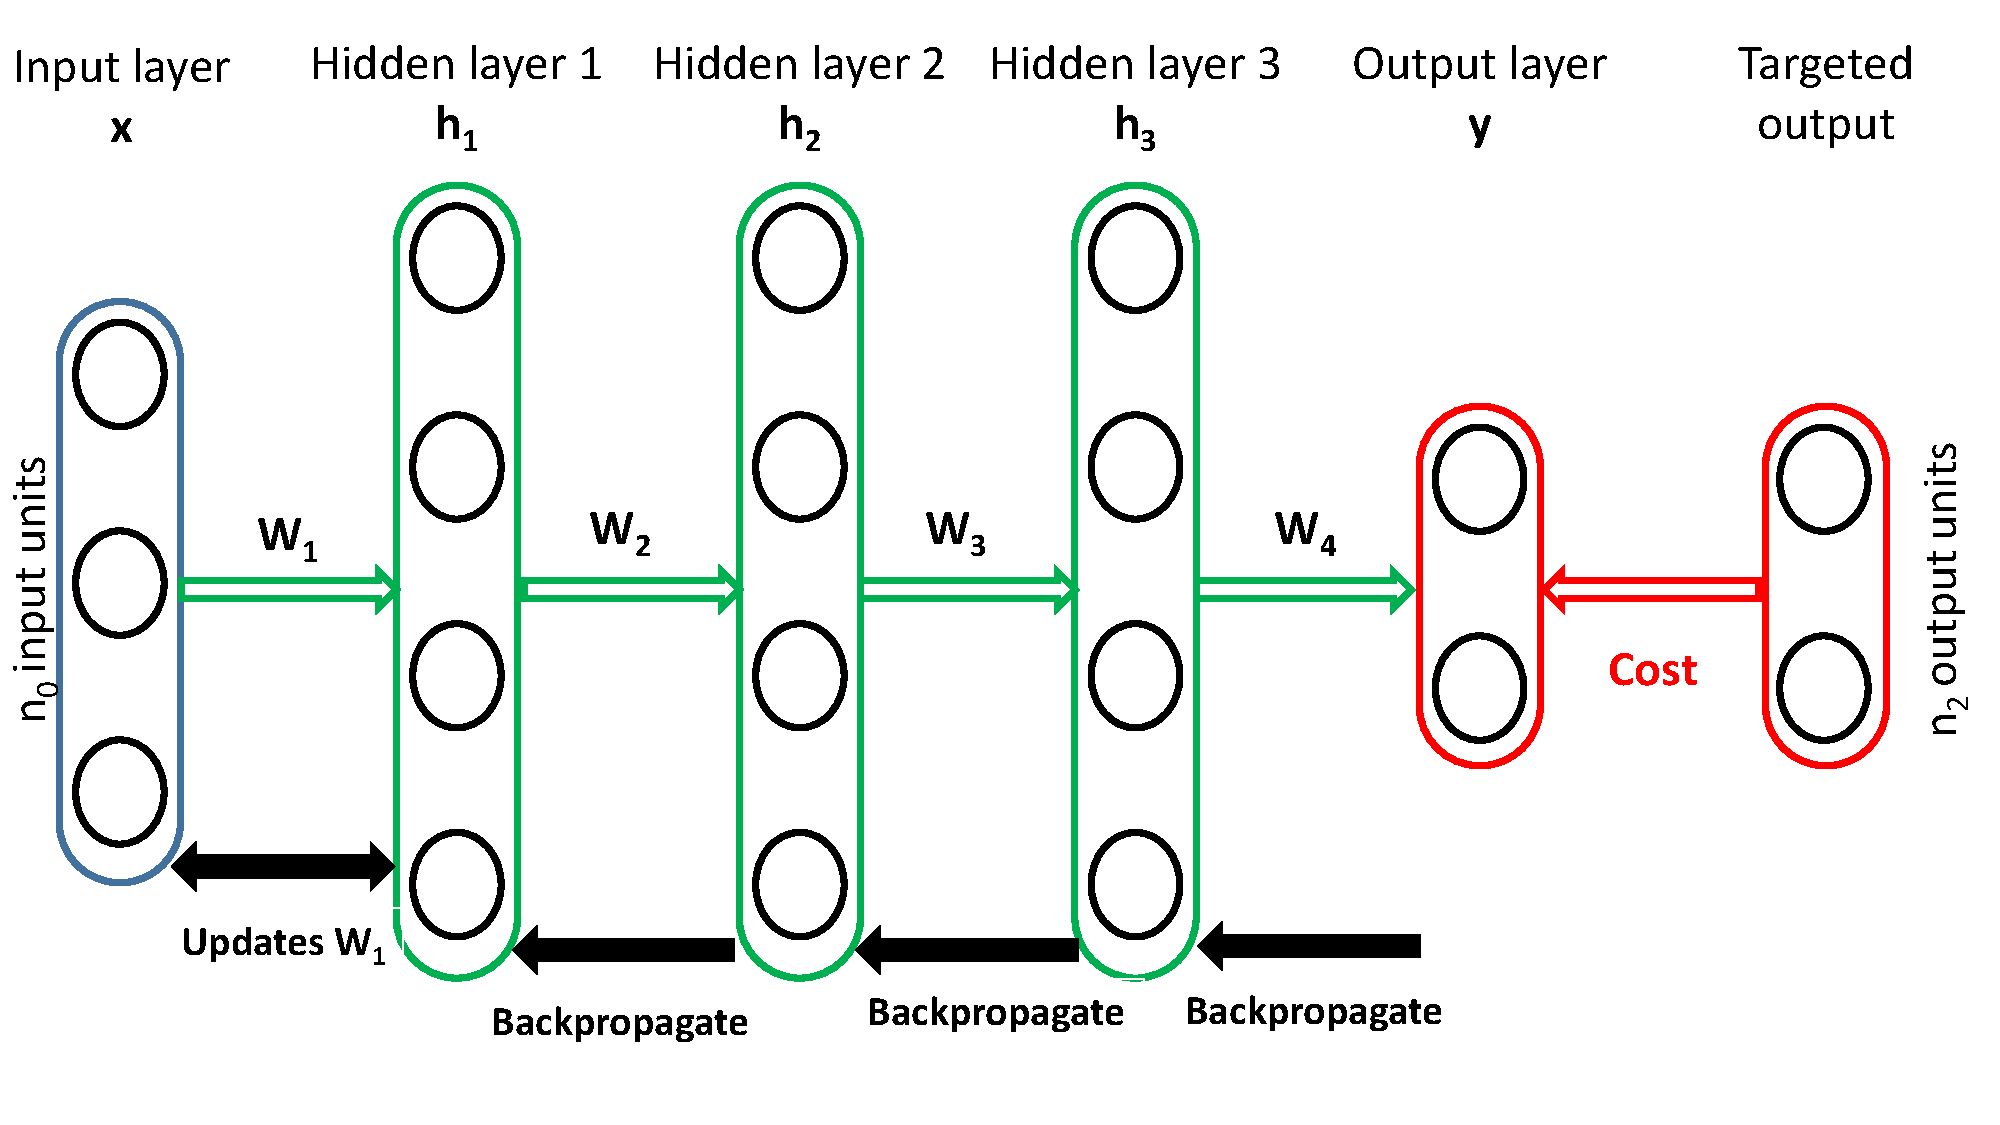
\includegraphics[width=3.5in,height= 1.5in]{Images/DNN/deep_MLP.pdf}
% 					\caption[A deep multi-layer perceptron]{Deep network trained by direct error backpropagation: The lower layers receive error signals that are diluted through repeated signal averaging by multiple layers of units with high fan-in leading to a poor learning quality}
% 					\label{fig:Deep multilayer perceptron}
% 				\end{center}
% 			\end{figure}      
%       
% 			One could argue that given a sufficient amount of training examples, the gradient descent will eventually affects the lower layers. However it appears that the gradient back propagated to the lower layers is not sufficient to move the parameters from their random initialization to an optimal state. It means that the \Important{gradient becomes less informative} about the change on the parameters to be made to move toward the optimum as it is propagated toward the lower layers, or that the error function -optimization objective- becomes too ill-conditioned for a gradient descent to escape apparent local minima. A deep architecture has an extensive parameter space, whereby searching for an ideal solution is challenging not only due to the non-convex supervised optimization problem and multiple local minima but also as the performances of the optimization strategy strongly depends on parameter initialization \cite{Erhan_2009}.
% 			
% 		\subsection{The training procedure:}
% 			\label{subseq:Deep neural networks/The training procedure/The training procedure}
%       
% 			\subsubsection{Greedy layer-wise unsupervised training:}
% 				As we have seen, training a deep neural network using directly the error back propagation over the whole network does not provide a  well trained predictor. But this training method does not really match the objective given for the deep architecture in the introduction of this report. Indeed the objective stated was to learn at each level a new representation of the input data. To do so, rather than using an error backpropagation over the whole network, it seems more adapted to train the layers one at the time -one representation at the time- from the bottom of the network to its top using the data processed through the already trained lower layers as training inputs -the representation of the input so far.\\\par
%       
% 				In 2006, Geoffrey Hinton \cite{Hinton_2006b} describes a recursive training procedure for a certain type of deep neural network -\Important{Deep Belief Network} (chapter~\ref{chap:Deep neural networks})- called \Important{greedy layer-wise unsupervised pre-training}. Shortly after, Marc'Aurelio Ranzato \cite{Ranzato_2006} and Yoshua Bengio \cite{Bengio_2007} have described the same type of procedure for other types of deep neural networks (respectively encoder-decoders and \Important{auto-encoders}). The three methods rely on  training individually shallow unsupervised modules and stacking them, one layer at a time from the bottom-up. When a new layer is stacked above the existing network, the parameters bridging the existing representation with a new layer are trained locally within the model using the previous layer as its inputs \cite{Bengio_2007, Geman_1984}.\\\par
%         
% 				For a train set $\mathcal{D}_{train}$, the procedure of this greedy learning algorithm to train a deep network with $d$ unsupervised layers $[\mathbf{h_{i}}]_{i \in [0,d-1]}$ is described by the algorithm~\ref{algo:Unsupervised greedy layer-wise learning algorithm}.\\\par
%         
% 				\begin{center}
% 					\begin{algorithm}[H]
% 						Initialize the input layer $\mathbf{x} \leftarrow \mathcal{D}_{train}$ \\
% 						\For{$l= 1 \text{ to } d-1$}{
% 							Initialize randomly $W_{l}$\\
% 							\While{Convergence == False}{
% 								Update $W_{l}$ by learning from $h_{l}$ -unsupervised learning\\
% 								\If{Convergence criteria is validated}{
% 									Convergence= True
% 								}
% 							}
% 							Fix $W_{l}$ and generate samples for $h_{l +1}$
% 						}
% 						\caption{Unsupervised greedy layer-wise learning algorithm}
% 						\label{algo:Unsupervised greedy layer-wise learning algorithm}		
% 					\end{algorithm}        
% 				\end{center}
%       
% 				Thus Hinton's idea is to split the deep network into several one layer neural networks. Those basic building blocks are then trained successively using an unsupervised approach. The optimization problems to be solved are then way more simple as they only involve shallow networks. The blocks are then assembled to create our deep neural network. Stacking the layers learned as a 1-layer neural network encourages higher-level abstractions of the input data within the internal representations of the deep architecture.   
% 
% 			\subsubsection{Supervised fine-tuning:}
% 			
% 				\begin{figure}[H]
% 					\begin{center}
% 						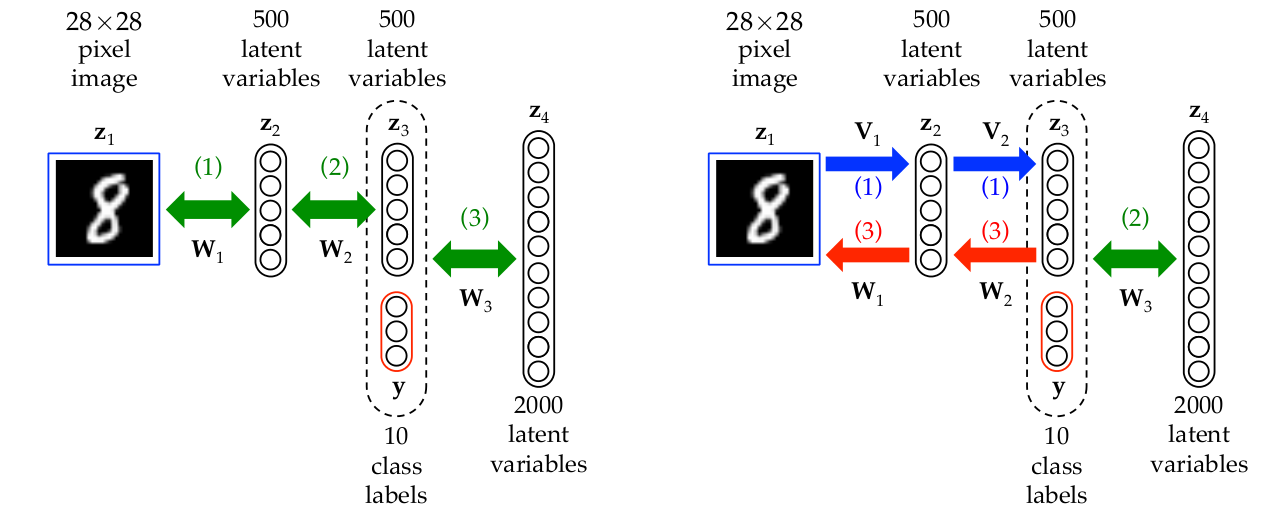
\includegraphics[width=4in,height=2in]{Images/DNN/DNN_trainingProcedure.png}
% 						\caption[Training of a deep neural network]{The two step training procedure of a deep neural network: First a generic unsupervised pre-training, followed by a task specific supervised fine-tuning}
% 						\label{fig:Training of a deep neural network}
% 					\end{center}
% 				\end{figure} 
% 
% 				Even though the greedy layer-wise unsupervised training strategy alone provides fairly good results on some discriminative or generalization tasks \cite{Hinton_2007}, if one want to use a deep neural network to tackle a classification problem, then the greedy layer-wise unsupervised training is used generally used as a \Important{pre-training step to initialized the parameters of our network} prior to a supervised training phase. Thus, in order to specialize the deep network, one can perform a supervised learning phase. It will fine-tuned the parameters of the deep neural network to bide it to a specific classification task.\\\par
% 				
% 				While the unsupervised pre-training is performed in a greedy layer-wise manner, the supervised fine tuning optimize the whole network at the same time. The most commonly used method to introduce labeled information into the deep neural network is through a discriminative learning using the error backpropagation algorithm \cite{Hinton_2006} described section~\ref{seq:Artificial neural networks/Multilayer perceptron network}.\\\par
% 				
% 				Although it has been observed that the error backpropagation algorithm did not provide good performances if used directly on a deep neural network with randomly initialized parameters, the same algorithm used on a model whose parameters have been initialized by a unsupervised pre-training yield to the state of the art performances obtained for deep neural networks. Indeed, the unsupervised pre-training helps the overall optimization by initializing the parameters around a good minimum \cite{Larochelle_2009}, easing the difficult deep supervised optimization problem. This has a regularization effect for subsequent supervised training by improving generalization \cite{Erhan_2009, Erhan_2010}.\\\par
% 			
% 				Thus the procedure to train a deep neural network for a specific classification task on a labeled dataset $\mathcal{D}_{train}= \left[x_{i},y_{i}\right]$, is describe by the algorithm~\ref{algo:Training of a deep neural network}.\\\par
%         
% 				\begin{center}
% 					\begin{algorithm}[H]
% 						\Important{-Unsupervised pre-training:} \\
% 						Perform a greedy layer-wise unsupervised pre-training on the data as described by the algorithm~\ref{algo:Unsupervised greedy layer-wise learning algorithm}\\
% 						\Important{-Supervised fine-tuning:} \\
% 						Using the parameters learned by the pre-training to initialized the network, fine-tune the network by using the error backpropagation algorithm (see the section~\ref{seq:Artificial neural networks/Multilayer perceptron network})
% 						\caption{Training of deep neural network}
% 						\label{algo:Training of a deep neural network}		
% 					\end{algorithm}        
% 				\end{center}
% 			
% 				One can notice that the labels are only used for the fine-tuning phase. Thus, the network obtained at the end of the unsupervised learning phase has learned a generic higher level representation of the input data. If required, this generic representation can then be fine-tuned with different objectives (classification, regression...).\\\par
% 				
% 				The two following chapter will introduce more deeply two types of building blocks for deep neural networks, the Restricted Boltzmann Machines (RBMs) and the associated Deep Belief Networks (DBNs - chapter~\ref{chap:DBN:}) and the Auto-Encoders (AEs) and the associated Stack Auto-Encoders (SAEs - chapter~\ref{chap:AE and SAE:}. The solution known as \Important{Encoder-Decoder} \cite{Ranzato_2006} using encoder-decoders as building block, will not be introduce at length in this document, mainly because not much work has been done on such networks during the internship and also because they are quite similar on the principle to the Auto-encoders.

				
%%%%%%%%%%%%%%%%%%%%%%%%%%%%%%%%%%%%%%%%%%%%%%%%%%%%%%%%%%%%%%%%%%%%%%%%%%%%%%%%%%%%%%%%%%%%%%%%%%%%%%%%%%%%%%%%%%%%%%%%%%%%%%%%%%%%%%%%%%%%%%%%%%%%
\chapter{Hidden Markov trees:}
\label{chap:DBN:}
	A \Important{Deep Belief Network} is built by stacking together \Important{Restricted Boltzmann Machines}, a simplified version of the Boltzmann machines (BMs). 	Thus to explain the training procedure of the RBMs, we will first briefly introduce the Boltzmann machines, then the RBMs and see what are the simplification yielded by the ``restriction'' done. Finally we will describe the unsupervised training procedure that has to be used in the greedy layer wise training algorithm~\ref{algo:Unsupervised greedy layer-wise learning algorithm} for RBMs.
	
	
  \section{Model:}
    \label{seq:DBN/The Boltzmann machine:}
    The Boltzmann machines  \cite{Hinton_1986} are a particular type of recurrent neural network with an energy-based model (i.e.: their dynamic is governed by energy functions). Specially, the probability density is given by the Boltzmann (i.e.: Gibbs) distributions. They are built out of $I$ stochastic binary units $x_{i}$ fully connected to each other, as illustrated in figure~\ref{fig:A Boltzmann machine}.
    
		\begin{figure}[H]
			\begin{center}
				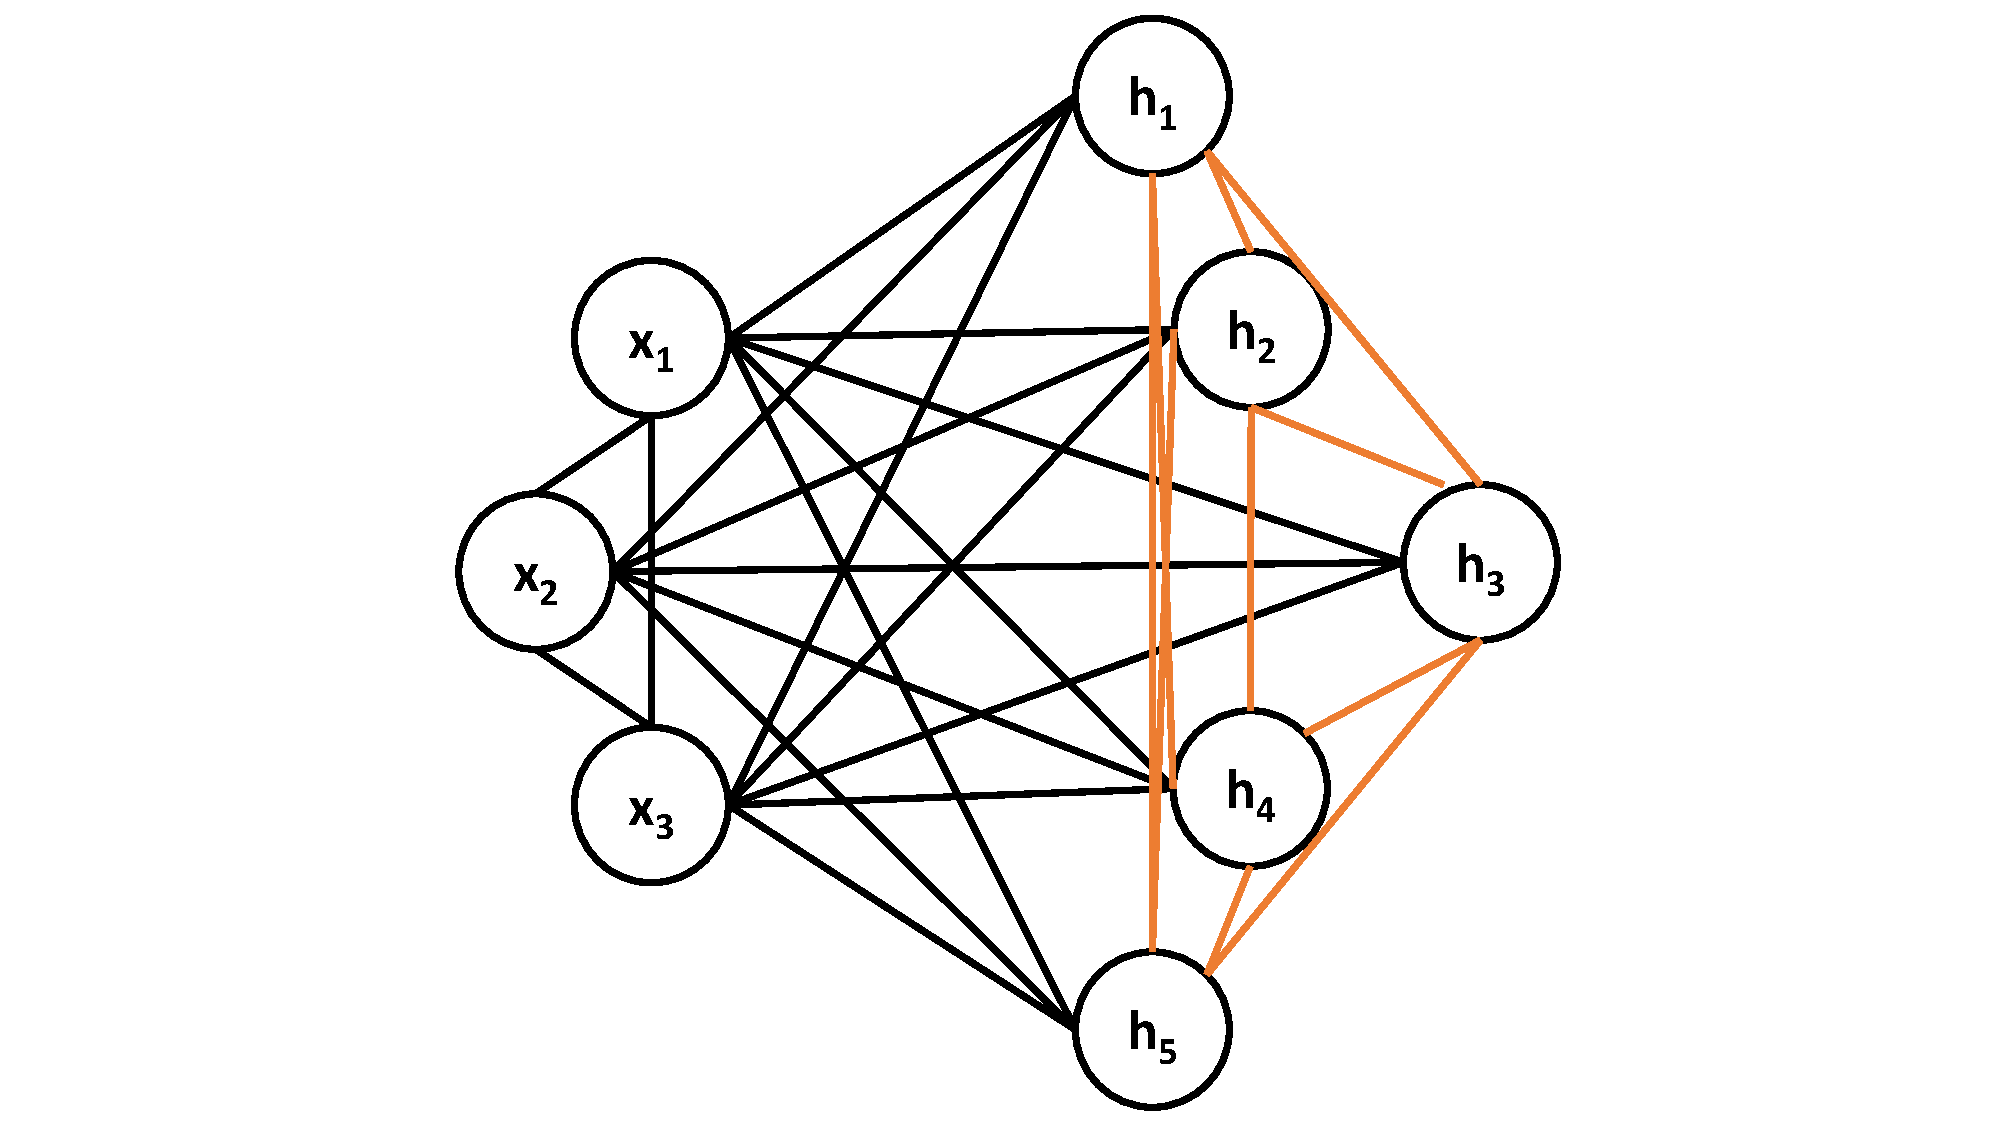
\includegraphics[width=2.5in]{Images/RBM_DNN/boltzmann_machine.pdf}
				\caption[A Boltzmann machine]{A Boltzmann machine: The ``input'' layer and the ``output'' layer are fully connected}
				\label{fig:A Boltzmann machine}
			\end{center}
		\end{figure}
		
		 Each unit $x_{i}$, connected to the others with the weights $\mathbf{W}$, has a probability of activation given by the sigmoid function:
		 
		\begin{equation}
			P(x_{i} = 1; \mathbf{W}) = \frac{1}{1 + \exp(-\sum_{j=0}^{I}{w_{ij}x_{j}})}
		\end{equation}\\
    
		Thus, the network provide a modeling of the probability of distribution of the input vectors $\mathbf{x}$ based on the Boltzmann/Gibbs distribution governed by the formula:
    
		\begin{equation}
			P(\mathbf{x}) = \frac{\exp(-E(\mathbf{x}))}{\sum_{\mathbf{x}}{\exp(-E(\mathbf{x}))}}
		\end{equation}\\
    
		where the energy function $E(\mathbf{x})$ is given by:
    
		\begin{equation}
			E(\mathbf{x})= - \sum_{i<j}(x_{i}w_{ij}x_{j})
			\label{eq:BM_energy}
		\end{equation}\\
    
		For a training set $\mathcal{D}_{train} = \{\mathbf{x}_{k}: k\in \left[1,\left|\mathcal{D}_{train}\right| \right]\}$, the learning seeks for the set of weights such as having a high average probability under the Boltzmann distribution for an input vector $\mathbf{x}_{k}$. For computational speed as well as accuracy, it is better to express the optimization of the probability in term of log-likelihood:
    
		\begin{equation}
			\begin{split}
				- \log(P(\mathbf{x}))	&= - \log\left(\frac{\exp(-E(\mathbf{x}))}{\sum_{\mathbf{x}}{\exp(-E(\mathbf{x})}}\right) \\
															&= - \log(\exp(-E(\mathbf{x}))) + \log\left(\sum_{\mathbf{x}}{\exp(-E(\mathbf{x}))}\right)
			\end{split}
    \end{equation}\\
    
    Indeed, taking the partial derivative of this expression with respect to $w_{ij}$ is simpler and we get:
    
		\begin{equation}
			\begin{split}
				- \left\langle \frac{\partial \log(P(\mathbf{x})}{\partial w_{ij}} \right\rangle_{data} 
										&= - \left\langle \frac{\partial \log(\exp(-E(\mathbf{x})))} {\partial {w_{ij}}} \right\rangle_{data} 
											+ \left\langle \frac{\partial \log\left(\sum_{\mathbf{x}}{\exp(-E(\mathbf{x}))}\right)}{\partial w_{ij}} \right\rangle_{model}\\
										&= \left\langle \frac{\partial E(\mathbf{x})} {\partial {w_{ij}}} \right\rangle_{data}
											- \left\langle \frac{\partial E(\mathbf{x})}{\partial w_{ij}} \right\rangle_{model} \\
										&= \left\langle x_{i}x_{j} \right\rangle_{data} - \left\langle x_{i}x_{j} \right\rangle_{model}
			\end{split}
			\label{eq:BM_derivative}
		\end{equation}\\  
    
		where $\left\langle.\right\rangle_{data}$ is the expectation of the input distribution, and $\left\langle.\right\rangle_{model}$ is the expectation of the stationary distribution of the model.\\\par
    
		Using the simplified derivative expression obtained in~\ref{eq:BM_derivative}, the weights can be updated using a gradient descent:
		
		\begin{equation}
			w_{ij} := w_{ij} + \epsilon \left( \left\langle x_{i}h_{j} \right\rangle_{data} - \left\langle x_{i}h_{j} \right\rangle_{model} \right)
			\label{eq:BM weight update}
		\end{equation}\\

		But while, in general, the term $\left\langle x_{i}h_{j} \right\rangle_{data}$ can easily be computed by sampling from the data distribution, there is \Important{no efficient way to directly compute the term $\left\langle x_{i}h_{j} \right\rangle_{model}$}. A estimate of the average over the sampled distribution $P(\mathbf{x})$ can be produce using a Markov Chain Monte Carlo approach to run the network to the equilibrium distribution. However, for a Boltzmann machine this process is very slow as it requires prolonged Gibbs sampling to explore the distribution $P(\mathbf{x})$ and reach the equilibrium state. Furthermore determining whether the distribution has reached an equilibrium state or not is challenging.
		
		
	\section{Learning: Expectation maximization:}
		\label{seq:DBN/The Restricted Boltzmann machine:}
    
		The difficulties experienced while training a Boltzmann machine are -at least partly- due to the fully-connected architecture that they present (figure~\ref{fig:A Boltzmann machine}). Thus the RBMs \cite{Smolensky_1986} have been introduced with the objective to ease the sampling problem while still being able to model interesting distributions. They are a particular form of bipartite log-linear Markov Random Field (i.e.:random field for which the energy function is linear in its free parameters). The modeling power is ensure by the bipartite property which suppose that some of the variables are never observed (hidden units). The number of hidden units of the machine is directly linked to its modeling capacities, the more hidden units, the better modeling capacity of the Boltzmann machine will be. Finally the restriction of a BM to an RBM is done by forcing to have \Important{no connection within the layers} (i.e.: no connection input-input nor hidden-hidden). The architecture of an RBM is presented 
figure~\ref{fig:A 
Restricted Boltzmann machine}.
    
		\begin{figure}[H]
			\begin{center}
				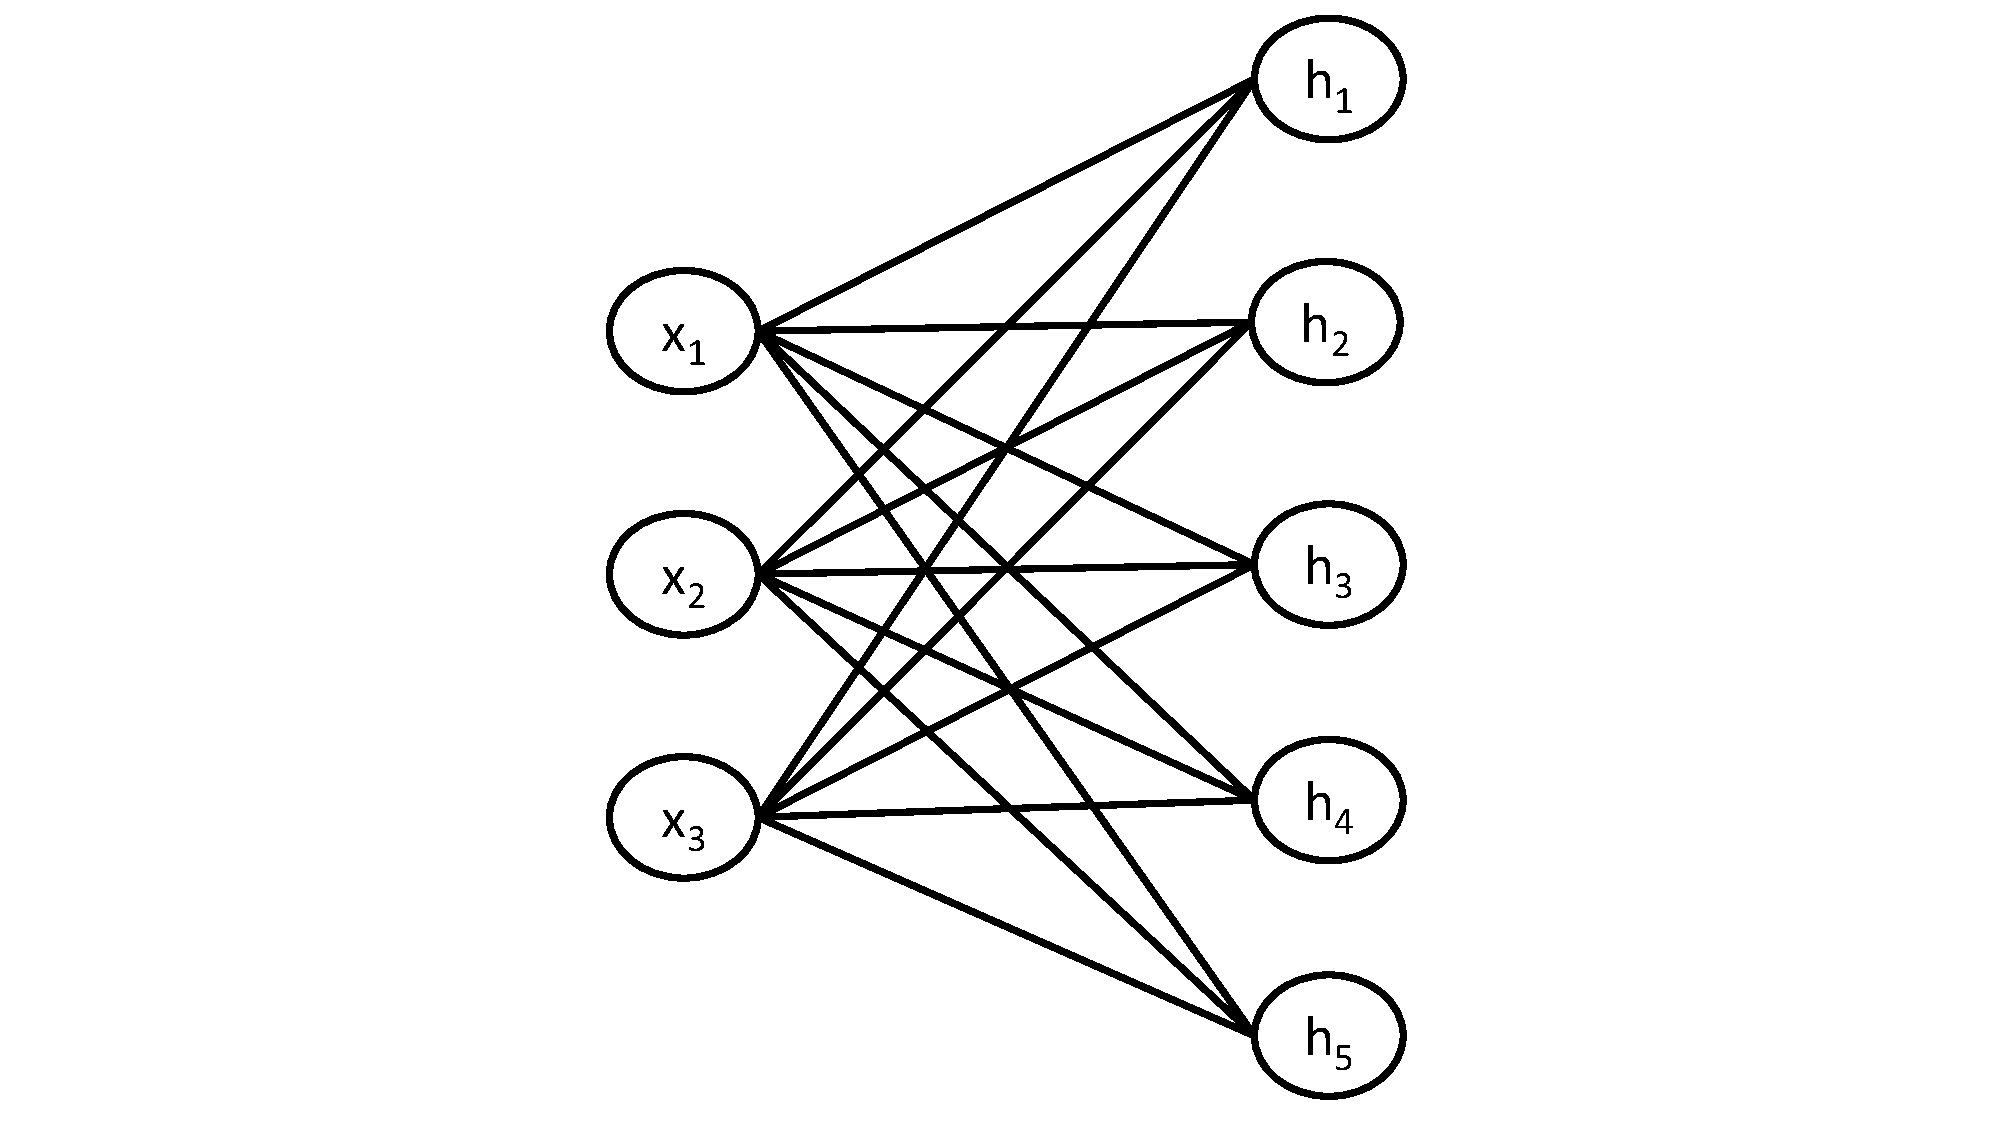
\includegraphics[width=2.5in]{Images/RBM_DNN/rbm.pdf}
				\caption[A restricted Boltzmann machine]{A Restricted Boltzmann machine: Compared to a Boltzmann machines the restriction imposes no  within layer connection (i.e.: no input-input nor output-output connection)}
				\label{fig:A Restricted Boltzmann machine}
			\end{center}
		\end{figure}
		
		Now let us consider a binary RBM with a visible input layer $\mathbf{x}$ of dimension $I$ (i.e.: size of the input vector) and an hidden layer $\mathbf{h}$ of dimension $J$ (i.e.: size of the output vector) as shown figure~\ref{fig:RBM for DBN}. Added to that, there are also offsets (i.e.: bias) units, $x_{0}$ and $h_{0}$ permanently set to one. The layers are associated by an undirected weight matrix $W$, such that every input unit $i$ is connected to every hidden variable $j$ via the weight $w_{ij}$.\\	
	
		\begin{figure}[H]
			\begin{center}
				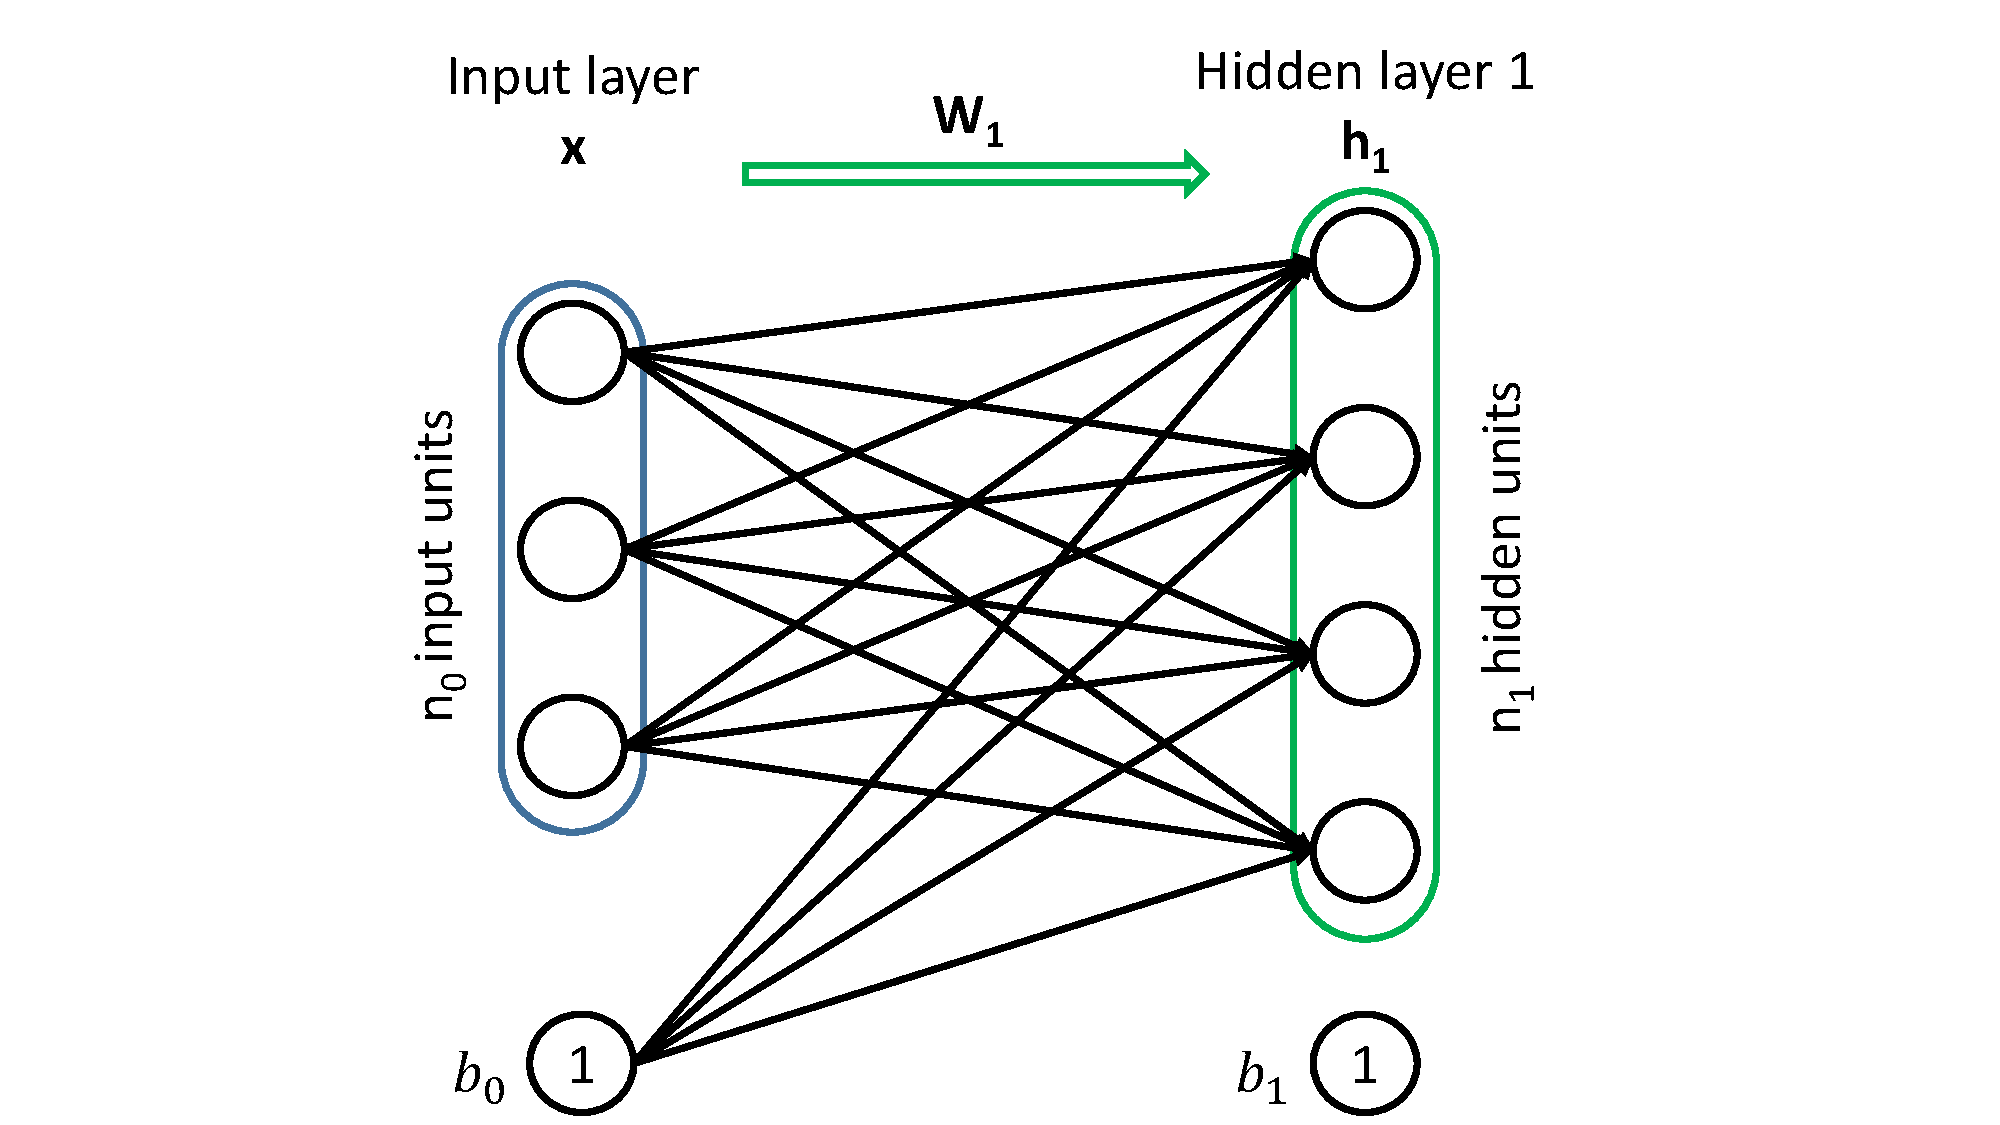
\includegraphics[width=2.5in]{Images/RBM_DNN/rbm_IJ.pdf}
				\caption[The structure of the restricted Boltzmann machine]{The RBM for machine learning connects an input layer $\mathbf{x}$ to a hidden layer $\mathbf{h}$ via undirected weights W and biases $x_{0}$ and $h_{0}$}
				\label{fig:RBM for DBN}
			\end{center}
		\end{figure}
		
		Because we have restricted the machine to a bipartite structure without intra-layer connections, the units of the hidden layer $\mathbf{h}$ are independent given the input layer $\mathbf{x}$. This independence simplify greatly the Gibbs sampling process compared to the Boltzmann machines. Thus, given an input vector, the activation probabilities of the hidden units of an RBM can be sampled by:
		
		\begin{equation}
			P(h_{j}=1 \mid \mathbf{x;W}) = \frac{1}{1 + \exp{(-\sum_{i=0}^{I}{w_{ij}x_{i}})}}
			\label{eq:RBM first sampling}
		\end{equation}\\
		
		Likewise, the input units can be sampled from the hidden vector using a symmetric decoder:
		
		\begin{equation}
			P(x_{j}=1 \mid \mathbf{h;W}) = \frac{1}{1 + \exp{(-\sum_{j=0}^{I}{w_{ij}h_{j}})}}
			\label{eq:RBM second sampling}		
		\end{equation}\\		
		
		In the case of a binary RBM, the energy of a the joint configuration $(\mathbf{x},\mathbf{h})$ of activation states $n$ the network defined in equation~\ref{eq:BM_energy} becomes: 
		
		\begin{equation}
			E(\mathbf{x},\mathbf{h}) = - \sum_{i=0}^{I}\sum_{j=0}^{J}x_{i}w_{ij}h_{j}
		\end{equation}\\
		
		Under the RBMs' assumptions, the joint probability distribution of states corresponding to the energy function $E(\mathbf{x},\mathbf{h})$ is modeled by a machine as follow:
		
		\begin{equation}
			P(\mathbf{x},\mathbf{h}) = \frac{\exp{(-E(\mathbf{x},\mathbf{h}))}}{\sum_{\mathbf{x},\mathbf{h}}{\exp{(-E(\mathbf{x},\mathbf{h}))}}}
		\end{equation}\\
		
		Where the denominator $\sum_{\mathbf{x},\mathbf{h}}{\exp{(-E(\mathbf{x},\mathbf{h}))}}$ is a normalization constant called the partition function. Following the maximum likelihood principle, the objective of the network is to maximize the marginal probability of the input vector $\mathbf{x}$ by summing over all possible vectors possible for the hidden layer $\mathbf{h}$:
		
		\begin{equation}
			P(\mathbf{x}) = \frac{\sum_{\mathbf{h}}{\exp{(-E(\mathbf{x},\mathbf{h}))}}}{\sum_{\mathbf{x},\mathbf{h}}{\exp{(-E(\mathbf{x},\mathbf{h}))}}}
		\end{equation}\\
		
		When given a training set $\mathcal{D}_{train}$ of $N$ input vectors $\{\mathbf{x}_{k}: k \in [1, N]\}$, the objective of the learning is to find the set of weight parameters $\mathbf{W^{\ast}}$ that minimize the average negative log-likelihood of the input data. Which leads to:
		
		\begin{equation}
			\begin{split}
				\mathbf{W^{\ast}}	&= \argmin{\mathbf{W}} - \left\langle \log P(\mathbf{x}) \right\rangle_{data}\\
												&= \argmin{\mathbf{W}} - \left( \left\langle  \log \left(\sum_{\mathbf{h}}\exp(-E(\mathbf{x},\mathbf{h})) \right) \right\rangle_{data} 
														+ \left\langle  \log \left(\sum_{\mathbf{x,h}}\exp(-E(\mathbf{x},\mathbf{h})) \right) \right\rangle_{model} \right)
			\end{split}
		\end{equation}\\
		
		The partial derivative compute for the Boltzmann machines~\ref{eq:BM_derivative} still stand for the RBMs and we have the following expression for the weight updates:
		
		\begin{equation}
			w_{ij} := w_{ij} + \epsilon \left( \left\langle x_{i}h_{j} \right\rangle_{data} - \left\langle x_{i}h_{j} \right\rangle_{model} \right)
			\label{eq:RBM weight update}
		\end{equation}\\
		
		Where $\langle.\rangle_{dist}$ denotes the expectation under the distribution \textit{dist}. The first term increases the probability of data driven activations that are clamped by the environment, while the second term reduces the probability of model driven states are sampled from the equilibrium distribution of a free running network. The weight update expressions are both the same for BMs~\ref{eq:BM weight update} and the RBMs~\ref{eq:RBM weight update}. However in the case of the RBMs there is an easy way to implement sampling strategy to compute an approximation of the term $\left\langle x_{i}h_{j} \right\rangle_{model}$.
	
	
	\section{Generation: Vitterbi algorithm:}
		\label{seq:DBN/Training with contrastive divergence:}

		The task of minimizing the average negative log-likelihood of the data distribution is equivalent to \Important{minimizing the Kullback-Leibler (KL) divergence} \cite{Kullback_1951} between the data distribution $P_{0}(\mathbf{x})$ (at time $t=0$) and the equilibrium distribution $P_{\infty}(\mathbf{x})$ (at time $t=\infty$):
		
		\begin{equation}
			D_{KL}(P_{0}\|P_{\infty}) = \sum_{(\mathbf{x},\mathbf{\hat{y}})} {P_{0}(\mathbf{x},\mathbf{\hat{y}}) \log \frac{P_{0}(\mathbf{x},\mathbf{\hat{y}})}{P_{\infty}(\mathbf{x},\mathbf{\hat{y}})}} \geq 0
		\end{equation}\\
		
		Geoffrey Hinton \cite{Hinton_2002} proposed the \Important{contrastive divergence learning algorithm}, that approximates the equilibrium distribution with a small finite number of sampling steps (Hinton's original paper use a number of step $N=1$). The Markov chain is relaxed to run for $N$ sampling steps to generate a reconstruction of the data vectors. An illustration of the sampling approximation is displayed in the figure~\ref{fig:Gibbs sampling}. The optimization seeks to minimize the difference between the two divergences:
		
		\begin{equation}
			CD_{N} = D_{KL}(P_{0}\|P_{\infty}) - D_{KL}(P_{N}\|P_{\infty}) \geq 0
		\end{equation}\\
		
		\begin{figure}[H]
			\begin{center}
				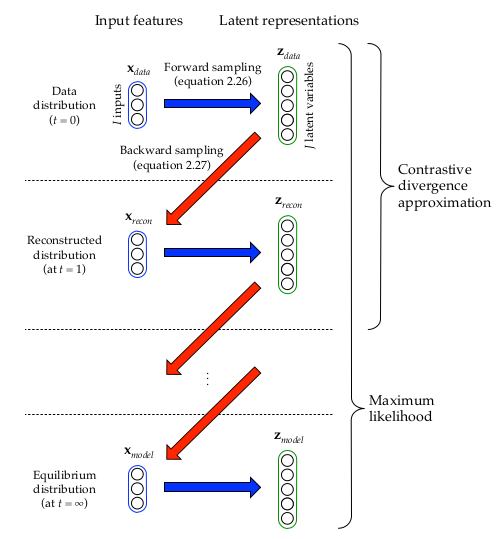
\includegraphics[width=3.5in]{Images/RBM_DNN/gibbs_sampling.png}
				\caption[The Gibbs sampling procedure]{Gibbs sampling relaxation of contrastive divergence learning. The maximum likelihood of the data distribution can be obtained by performing alternating (forward-backward) Gibbs sampling between the input layer x and latent layer h, from the data distribution samples (at $t=0$) until $t=\infty$. The contrastive divergence approximates the equilibrium distribution using reconstructed samples from a small finite number of sampling steps. One sampling step (N = 1) is used in this example.}
				\label{fig:Gibbs sampling}
			\end{center}
		\end{figure}
		
		The partial derivative with respect to the parameter $w_{ij}$ is:
		
		\begin{equation}
			\begin{split}
				\frac{\partial CD_{N}}{ \partial w_{ij}} 
									&= \frac{\partial D_{KL}(P_{0}\|P_{\infty})} {\partial w_{ij}} - \frac{\partial D_{KL}(P_{N}\|P_{\infty})} {\partial w_{ij}}  \\
									&\approx - \left\langle \frac{\partial \log \sum_{x}{\exp{(-E(\mathbf{x,h}))}}}{\partial w_{ij}} \right\rangle_{data} +
													\left\langle \frac{\partial \log \sum_{x}{\exp{(-E(\mathbf{x,h}))}}}{\partial w_{ij}} \right\rangle_{recon} \\
									&\approx \left\langle \frac{\partial E(\mathbf{x,h})}{\partial w_{ij}} \right\rangle_{data} - \left\langle \frac{\partial E(\mathbf{x,h})}{\partial w_{ij}} \right\rangle_{recon} \\
									&\approx \left\langle x_{i}h_{j} \right\rangle_{data} - \left\langle x_{i}h_{j} \right\rangle_{recon}
			\end{split}
		\end{equation}\\
		
		Where $\langle.\rangle_{recon}$ is the expectation of the reconstructed states after $N$ sampling steps. Using those partial derivative, one can approximates the gradient descent by:
		
		\begin{equation}
			w_{ij} := w_{ij} + \epsilon \left( \left\langle x_{i}h_{j} \right\rangle_{data} - \left\langle x_{i}h_{j} \right\rangle_{recon} \right)
			\label{eq:CD weight update}
		\end{equation}\\

		Where the energy of samples from the data distribution is decreased, while raising the energy of reconstructed states that the network prefers to real data.\\\par
		
		The algorithm~\ref{algo:RBM training with CD} presents the iterative procedure for training an RBM with $N$ Gibbs sampling steps followed by the updates of the parameters.\\
		
		\begin{center}
			\begin{algorithm}[H]
				1) Initialize $\mathbf{W}$\\
				2) \While{no convergence:}{
					Get $\mathbf{x}_{0}$ from randomized training batches.\\
					Sample $P_{0}(\mathbf{h_{0}}\mid\mathbf{x_{0}})$ using~\ref{eq:RBM first sampling} 
					3) \For{$n=1 \text{to} N$}{
						Sample $P_{n}(\mathbf{x_{n}}\mid\mathbf{h_{n-1}})$ using~\ref{eq:RBM second sampling}\\
						Sample $P_{n}(\mathbf{h_{n}}\mid\mathbf{x_{n}})$ using~\ref{eq:RBM second sampling}
					}
					Update $w_{ij} := w_{ij} + \Delta w_{ij}$ using~\ref{eq:CD weight update}
					}
				\caption{RBM training with $N$ steps contrastive divergence.}
				\label{algo:RBM training with CD}		
			\end{algorithm}
		\end{center}
		
		$CD_{1}$ is the fastest training procedure for RBMs has it requires the minimal number of sampling steps. Most of the time, it provides a good approximate of the distribution. Although a greater number of sampling steps will produce an estimate closer to the true likelihood of the gradient, it will need more computational time and may results in high estimator variance \cite{Hanlin_2013}.
		
		
% 	\section{Deep belief networks:}
% 		\label{seq:DBN/Deep belief networks:}
% 		Deep Belief Network (DBN) \cite{Hinton_2006} is a \Important{probabilistic graphical model} built of a hierarchy of stochastic latent variables using restricted Boltzmann machines (RBMs) as the basic building block. As the multi-layer perceptron (see section~\ref{seq:Artificial neural networks/Multilayer perceptron network}), the DBNs have been shown to be be universal approximators \cite{LeRoux_2008}.\\\par
% 		
% 		The piling of RBMs to create a DBN is a straight forward procedure. For a deep belief network of depth $d$, the $RBM^{(l)}$ is trained using the the representation $\mathbf{h^{(l-1)}}$ generated by the $RBM^{(l-1)}$ as training examples (figure~\ref{fig:Training of a deep neural network}  for a illustration of the stacking procedure for DBNs).
% 		
		
%%%%%%%%%%%%%%%%%%%%%%%%%%%%%%%%%%%%%%%%%%%%%%%%%%%%%%%%%%%%%%%%%%%%%%%%%%%%%%%%%%%%%%%%%%%%%%%%%%%%%%%%%%%%%%%%%%%%%%%%%%%%%%%%%%%%%%%%%%%%%%%%%%%%
\chapter{Scattering hidden Markov tree:}
	\label{chap:AE and SAE:}
	The \Important{Stack Auto-Encoders} (SAEs) are another type of deep neural architecture exploiting the \Important{Auto-Encoders} (AEs) as building blocks. As we will see in the following section~\ref{seq:AE and SAE/Training procedure:}, the training procedure for AEs is easier to implement than the RBMs (section~\ref{seq:DBN/Training with contrastive divergence:}) one. So they have also been used as building blocks to train deep neural networks, where each level is associated with an auto-encoder that can be trained separately \cite{Larochelle_2007, Ranzato_2007, Vincent_2008,Bengio_2007}.
	
	
	\section{Hypothesis:}
		\label{seq:AE and SAE/AEs:}
		An auto-encoder is a multi-layer perceptron (section~\ref{seq:Artificial neural networks/Multilayer perceptron network}) with one hidden layer trained to encode an input $\mathbf{x}$ into some representation $\mathbf{h(x)}$ so that the input can be reconstructed (i.e.: decoded) from that representation to produce the output layer. \\\par
		
		\begin{figure}[H]
			\begin{center}
				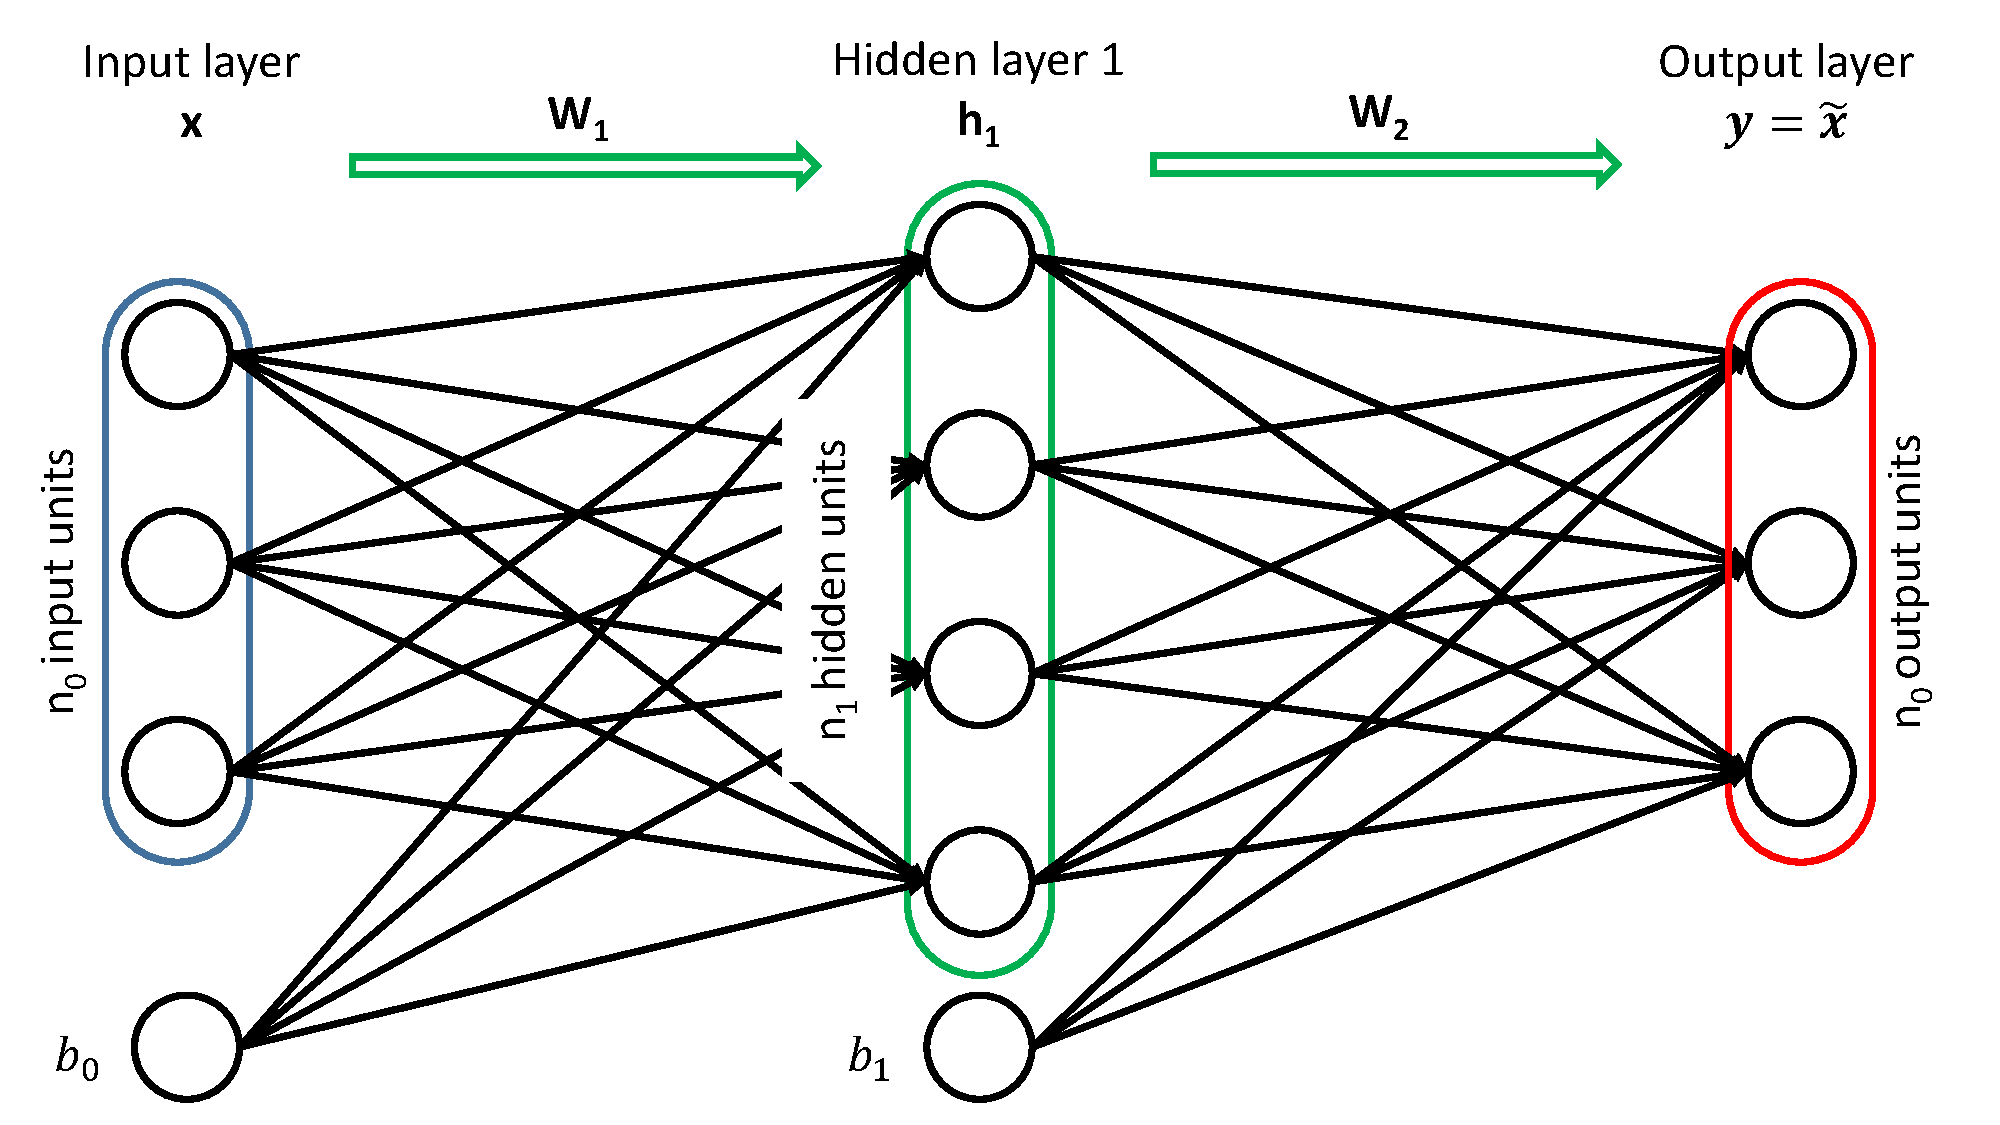
\includegraphics[width=3.5in]{Images/AE_SAE/AE.pdf}
				\caption[An auto-encoder]{An auto-encoder: Maps an input $\mathbf{x}$ to a representation $\mathbf{h_{1}}$ with the objective to compute the best reconstruction $\mathbf{\hat{y}} = \mathbf{\tilde{x}}$ for the output layer of the network.}
				\label{fig:AE}
			\end{center}
		\end{figure}
				
		Given a train set $\mathcal{D}_{train}$ of $m$ elements living in $[0,1]^{d}$, an auto-encoder takes an input $\mathbf{x}$ and maps it \Important{deterministically}, via an encoder, to an hidden representation $\mathbf{h(x)} \in [0,1]^{d'}$ following the relation:
		
		\begin{equation}
				\mathbf{h} = \sigma_{1}(W_{1}.\mathbf{x} + b_{1}) = \sigma_{1}(W_{1},b_{1},\mathbf{x}) = a_{1}(\mathbf{x})
		\end{equation}\\
		
		Where $\sigma$ is the activation function for the hidden unit (section~\ref{seq:Artificial neural networks/Perceptron network}). The latent representation (i.e.: code) $\mathbf{\hat{y}}$ is then mapped back, via a decoder, into a reconstruction $\mathbf{\hat{y}}$ of the same shape as $\mathbf{x}$ by a similar transformation:
		
		\begin{equation}
				\mathbf{\hat{y}} = \sigma_{2}(W_{2} \mathbf{h} + b_{2}) = \sigma_{2}(W_{2},b_{2},\mathbf{h}) = a_{2}(\mathbf{h})
		\end{equation}\\
		
		Thus, $\mathbf{\hat{y}}$ is the prediction of $\mathbf{x}$ given the code $\mathbf{h}$ and we have:
		
		\begin{equation}
				\mathbf{\hat{y}} = \sigma_{2}(W_{2}, b_{2}, \sigma_{1}(W_{1}, b_{1}, \mathbf{x})) = a_{2}(a_{1}(\mathbf{x}))
		\end{equation}\\

		The auto-encoder tries to learn a function $f(W_{1},b_{1},W_{2},b_{2},\mathbf{x}) \approx \mathbf{x}$. In other word, it is trying to learn an approximation of the identity function so that the output $\mathbf{\hat{y}}= \mathbf{\tilde{x}}$ is similar to $\mathbf{x}$. Stated like this, one could argue that the identity function appears to be a particularly trivial function to be learned. But by \Important{placing constraints on the network}, such as  reducing the number of neurons for the encoded representation of the inputs (i.e.: number of neurons in the hidden layer), interesting representation can be learned. For example, suppose that the training data are a set of 28 x 28 gray-scale images (784 pixels/image) described by the pixel intensity. Hence, the input layer $L^{(0)}$ of the auto-encoder has $n^{(0)} = 784$ units and suppose we are trying to encode it using a hidden layer $L^{(1)}$ with $n^{(1)} = 196$ units. Note that the AE's properties imposed to have an output layer $L^{(2)}$ with  $n^{(3)} = 
784$. Since the number of units available to learn the 
representation of the input is four times smaller than the input size, the network is forced to learn a compressed representation of the input (i.e.: given the vector of hidden units $h(x) \in \mathbb{R}^{196}$, the network has to reconstruct the 784-pixel input $x$). In the case of random inputs, this compression task is very difficult. But if there is a structure in the data (e.g.: correlated features...), then the AE will be able to learn -at least part of- the structure to perform the compression. In fact, the simple auto-encoder used in this example often ends up learning a low-dimensional representation very similar to PCA's \cite{Ng_course}. \\\par
		
		Even if the above argument relied on the number of neurons $n^{(1)}$ in the hidden unit to be smaller than the number of input neurons $n^{(0)}$, it is still possible to discover interesting structure in the data with a network with more hidden units than input units by imposing other constraints on the auto-encoder (chapter~\ref{chap:Regularization methods for Auto-encoders} for more details about the regularization methods).
				
				
	\section{Results and application:}
		\label{seq:AE and SAE/Training procedure:}
		
		The goal being to recreate the input, the parameters $\mathbf{W_{1}}, \mathbf{W_{2}}, \mathbf{b_{1}}, \mathbf{b_{2}}$ of the auto-encoder are optimized in order to minimize the average reconstruction error $J$. The definition of $J$ can vary depending on the problem assessed:\\
		
		\begin{itemize}
			\item \Important{Cross-entropy:} When the inputs are interpreted as bit vectors  or as vectors of bit probabilities it is better to use the cross-entropy function to measure the cost of the reconstruction. Its expression becomes for an auto-encoder trained on the dataset $\mathcal{D}_{train}$ define earlier in this chapter:
				\begin{equation}
					\begin{split}
							J(W_{1},W_{2},b_{1}, b_{2})
												&= -\frac{1}{m} \sum_{i=0}^{m-1} \sum^{d}_{k=1}\left(x_{ik} \log \hat{y}_{ik} + (1 - x_{ik})\log(1 - \hat{y}_{ik})\right)
												\\
												&= -\frac{1}{m} \sum_{i=0}^{m-1} \sum^{d}_{k=1}(x_{ik} \log(\sigma_{2}(W_{2}, b_{2}, \sigma_{1}(W_{1}, b_{1}, x_{ik}))) \\ 
													&\quad\quad\quad\quad + (1 - x_{ik})\log(1 - \sigma_{2}(W_{2}, b_{2}, \sigma_{1}(W_{1}, b_{1}, x_{ik}))))
						\end{split}
				\end{equation}\\
				
			\item \Important{Squared error:} The squared error is used for the classification or regression problems.
				\begin{equation}
					\begin{split}
						J(W_{1},W_{2},b_{1}, b_{2})
												&= -\frac{1}{m} \sum_{i=0}^{m-1} \left( \|\mathbf{x_{i}}-\mathbf{\hat{y}_{i}}\|^{2} \right) \\
												&= -\frac{1}{m} \sum_{i=0}^{m-1} \left( \|\mathbf{x_{i}}- \sigma_{2}(W_{2}, b_{2}, \sigma_{1}(W_{1}, b_{1}, \mathbf{x_{i}})   \|^{2} \right)
					\end{split}
				\end{equation}\\
				
			\item \Important{Personalize cost:} Another possibility is to define a metric tailored to the specific problem assessed. This metrics has to admit derivatives in order to allow its optimization.\\
		\end{itemize}
		
		The auto-encoder is then trained using the backpropagation algorithm described in the section~\ref{seq:Artificial neural networks/Training by error backpropagation}.					
		
		
% 	\section{Stack Auto-encoders:}
% 		\label{seq:AE and SAE/SAE:}
% 		
% 		Due to the fact that an auto-encoder is a three-layer perceptron the stacking of the auto-encoders to create a stack auto-encoders is slightly harder than the stacking of RBMs. Indeed, to describe the stacking procedure of auto-encoders we first need to introduce the following concepts:\\
% 		
% 		\begin{itemize}
% 			\item \Important{$AE_{encode}$:} This is the encoding part of an auto-encoder, transforming the input into its representation. It has the parameters $(W_{1}, b_{1}, \sigma_{1})$.\\
% 			
% 			\item \Important{$AE_{decode}$:} This is the decoding part of an auto-encoder, transforming the representation back into the input approximation. It has the parameters $(W_{2}, b_{2}, \sigma_{2})$.\\
% 			
% 			\item \Important{$SAE_{encode}[N]$:} This is the encoding part of a stack auto-encoder of depth $N$, transforming the input into its representation. It has the parameters $\left[(W_{i,1}, b_{i,1}, \sigma_{i,1})_{i \in [1, N]}\right]$.\\
% 			
% 			\item \Important{$SAE_{decode}[N]$:} This is the decoding part of a stack auto-encoder of depth $N$, transforming the representation back into the input approximation. It has the parameters $\left[(W_{i,2}, b_{i,2}, \sigma_{i,2})_{i \in [1, N]}\right]$.\\			
% 		\end{itemize}
% 		
% 		\begin{figure}[H]
% 			\begin{center}
% 				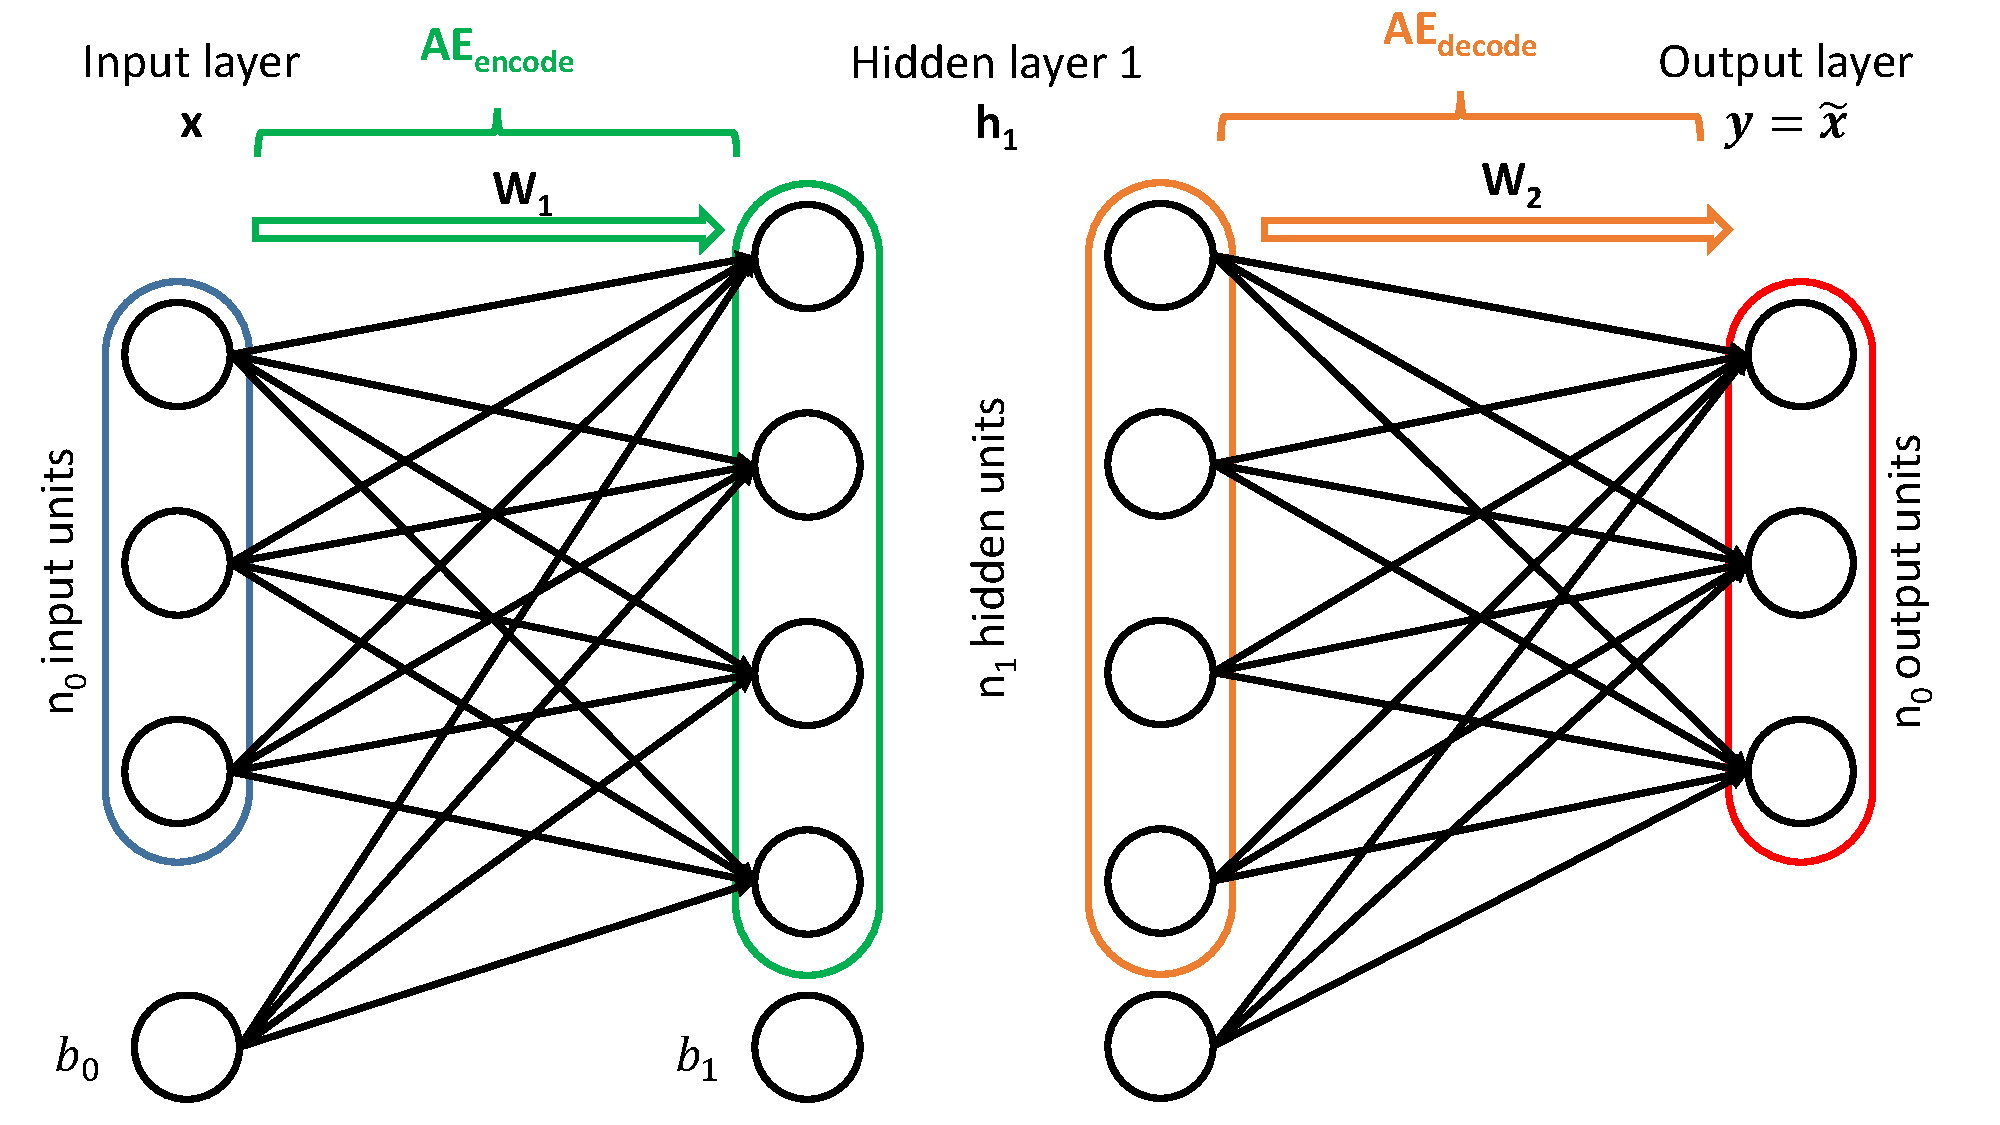
\includegraphics[width=3.5in]{Images/AE_SAE/AE_splitted.pdf}
% 				\caption{An encoder and a decoder}
% 				\label{fig:AE_splitted}
% 			\end{center}
% 		\end{figure}
% 
% 		Those elements defined the stacking procedure for a deep neural network of depth $N$ trained on a dataset $\mathcal{D}_{train}$ is described in algorithm~\ref{algo:Stacking AEs}:\\\par
% 		
% 		\begin{center}
% 			\begin{algorithm}[H]
% 				\For{$i$ in $[1,N]$:}{
% 					1) Propagate the inputs:\\
% 						\For{$x \in \mathcal{D}_{train}$}{
% 							Propagate $x$ through $SAE_{encode}[i]$ to create $x_{encode}[i]$ the representation of the input at depth $i$.\\
% 						}
% 					2) Train the $AE[i]$:\\
% 					Using $\mathcal{D}_{encode}[i] = [x_{encode}[i]]$ as a training set and following the procedure described in section~\ref{seq:AE and SAE/Training procedure:}.\\
% 					3) Stack $AE[i]$ on $SAE[i]$:\\
% 					\begin{itemize}
% 						\item Connect $AE_{encode}[i]$ to the top of $SAE_{encode}[i]$: 
% 							\begin{equation}
% 								SAE_{encode}[i+1] = SAE_{encode}[i] + AE_{encode}[i]
% 							\end{equation}\\
% 						\item Connect $AE_{decode}[i]$ to the bottom of $SAE_{decode}[i]$:
% 						\begin{equation}
% 							SAE_{decode}[i+1] = AE_{decode}[i] + SAE_{decode}[i]
% 						\end{equation}\\
% 					\end{itemize}
% 					}
% 				\caption{Stacking procedure for auto-encoders}
% 				\label{algo:Stacking AEs}		
% 			\end{algorithm}
% 		\end{center}
% 		
% 		\begin{figure}[H]
% 			\begin{center}
% 				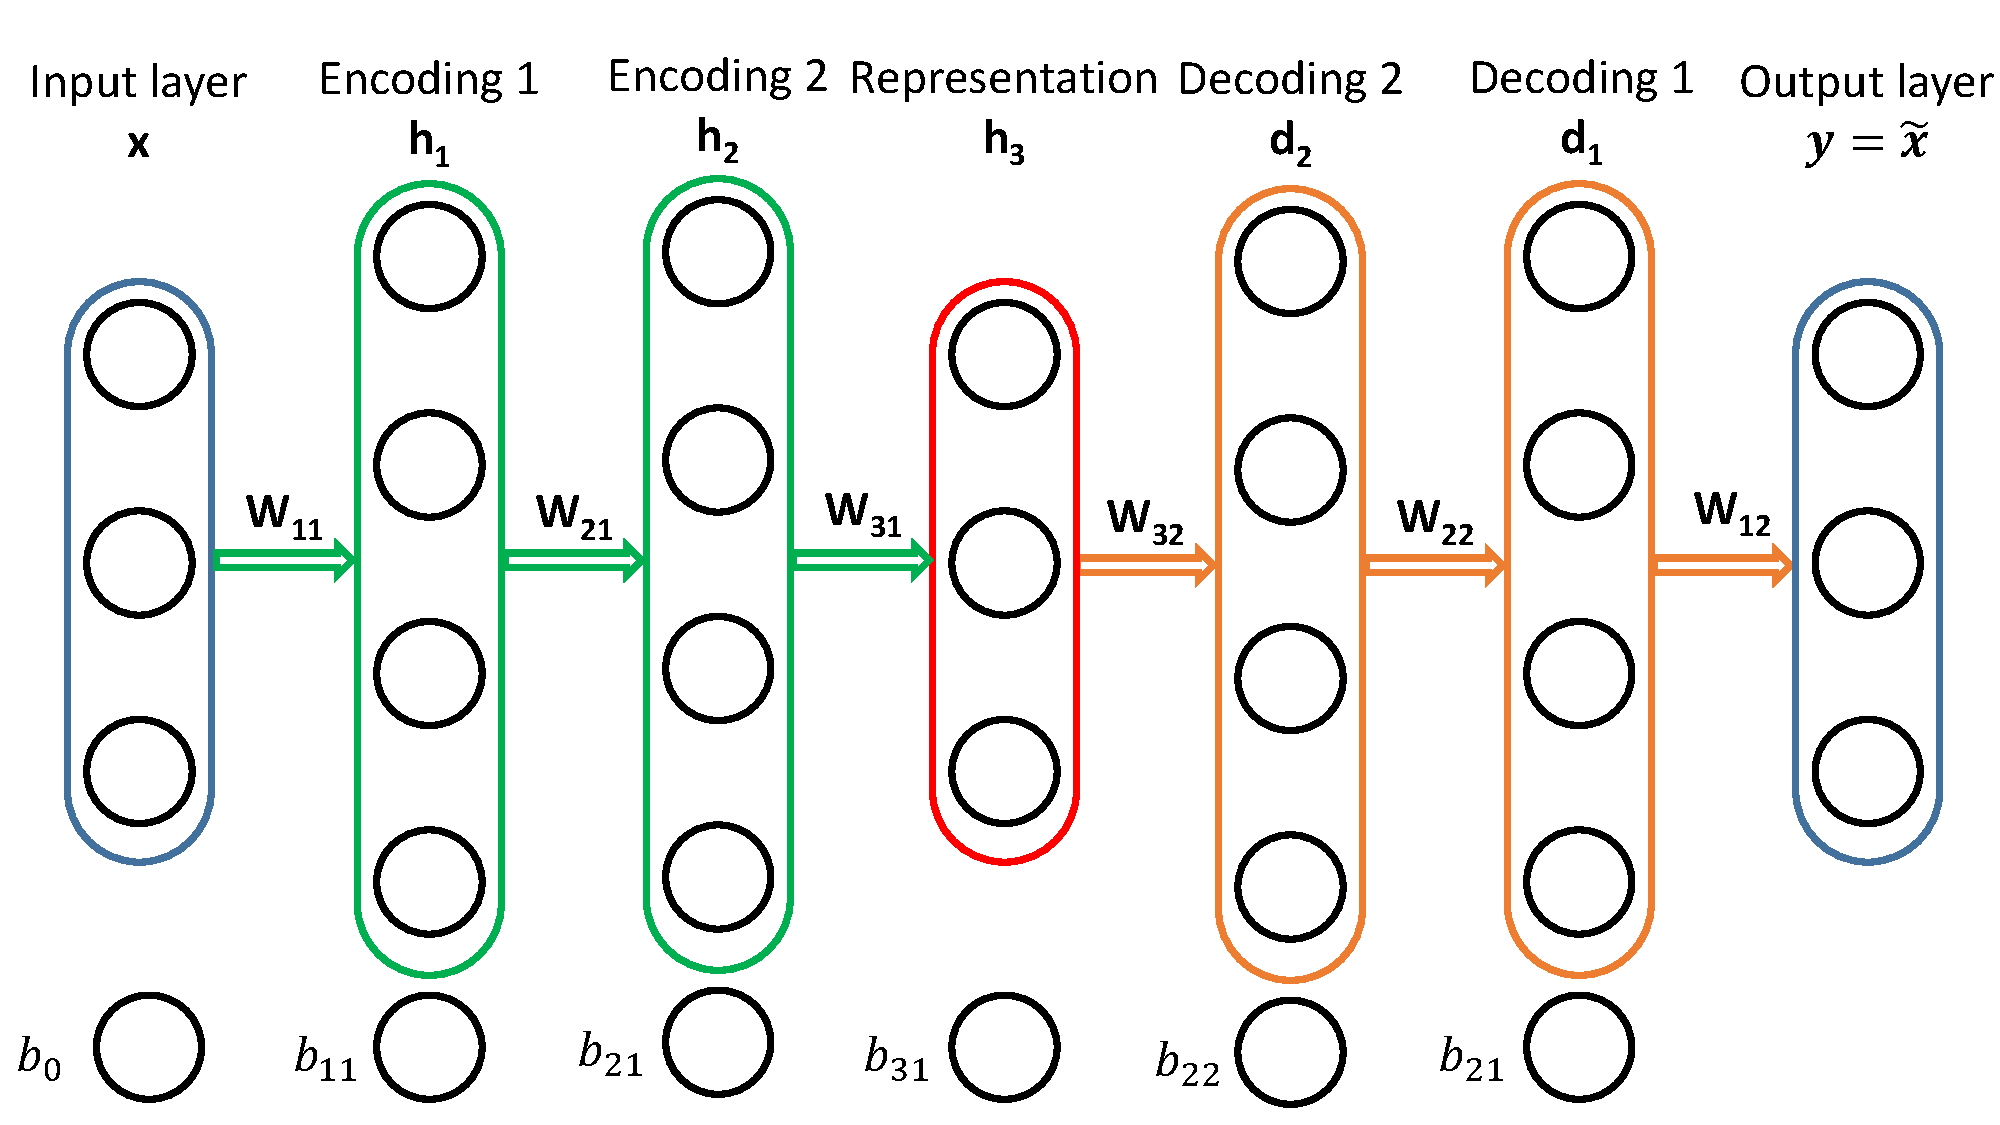
\includegraphics[width=3.5in]{Images/AE_SAE/SAE.pdf}
% 				\caption[A Stack Auto-Encoder]{A Stack Auto-Encoder: Maps successively an input $\mathbf{x}$ to representations $\mathbf{h_{i}}$ with the objective to compute the best reconstruction $\mathbf{\hat{y}} = \mathbf{\tilde{x}}$ for the output layer of the network.}
% 				\label{fig:SAE}
% 			\end{center}
% 		\end{figure}
% 		
% 
% %%%%%%%%%%%%%%%%%%%%%%%%%%%%%%%%%%%%%%%%%%%%%%%%%%
% %%%%%%%%%%%%%%%%%%%%%%%%%%%%%%%%%%%%%%%%%%%%%%%%%%
% \chapter{Regularization methods for Auto-encoders:}
% 	\label{chap:Regularization methods for Auto-encoders}
% 	A central issue when it comes to train a neural network (whether deep or shallow) is to determine the optimal degree of complexity for the model $\mathbf{h(x)}$. If a model too simple will not be able to capture sufficient of the structure in the data, on the other hand, a too complex one will lead to model the noise of the training data (i.e.: to over-fit). But in both case the generalization performances will be poor. This problem can be regarded as the search for the optimal \Important{trade-off between bias} (i.e.: model flexibility) \Important{and variance} (i.e.: model freedom) \cite{Geman_1992}.\\\par
% 	
% 	Several methods exist to control the bias/variance of a model. The most straight forward is the \Important{structural stabilization}. It involves making adjustments to the number of free parameters of the networkn for example by making adjustments on the number of neurons to be used. Another method, called \Important{regularization}, consists on adding a penalty term $\Omega(\mathbf{\hat{y}})$ to the error function $J$ to be minimized in order to reduce the variance of a relatively flexible model.
% 	
% 	\begin{equation}
% 		\tilde{J}= J + \lambda \Omega(\mathbf{\hat{y}})
% 	\end{equation}\\
% 	
% 	Where the parameter $\lambda$ control the bias/variance trade-off by affecting more or less influence to $\Omega(\mathbf{\hat{y}})$ over $J$ in the cost function to be minimized. The regularization function $\Omega(\mathbf{\hat{y}})$ is generally expressed in terms of the network function $\mathbf{\hat{y}(x)}$ and its derivatives. Several types of regularization function can be used depending on the application, later on we will see the most common ones for the auto-encoders.\\\par
% 	
% 	A third kind of methods the control the bias/variance trade-off is to add noise to the input data. Again we will see later on the effect of this methods applied to the auto-encoders. But we will first introduce a regularization method particular to the auto-encoders.\\\par
% 	
% 	A further point to note is the importance of the regularization for auto-encoders. Indeed, because they are basically trying to map the identity function (see section~\ref{seq:AE and SAE/AEs:}), without proper regularization, AEs are very likely to over-fit to the training data.\\\par
% 	
% 	Finally the examples provided in this section come from auto-encoders with an hidden layer of $1000$ units trained on the famous \Important{MNIST} dataset (see section~\ref{seq:Experimental results/MNIST:} for a details description of MNIST).
% 	
% 	
% 	\section{Tied weights:}
% 		\label{seq:Regularization methods for Auto-encoders/Tied weights:}
% 		This method is peculiar to the auto-encoders and lays into the structural stabilization category. The idea is to reduce the number of free parameters of the auto-encoder by imposing:
% 		
% 		\begin{equation}
% 			W_{2} = W_{1}^{T}
% 		\end{equation}\\
% 		
% 		This constrain  has an effect on the bias/variance trade-off as it reduce by a factor 2 the number of parameters the be optimized. It prevents as well degenerate solutions, in particular one with very small weights $W_{1}$ for the encoder, counter-balanced by very large weights $W_{2}$ for the decoder. Which is likely to occur, for example, in a near-linear solution to be learned with hyperbolic tangent activation function.\\\par
% 		
% 		A positive side effect when using this method is a great reduction of the memory footprint of the auto-encoder. Knowing the computational issues linked to deep neural networks, this advantage is precious.\\\par
% 		
% 		\begin{figure}[H]
% 			\begin{center}
% 				\begin{subfigure}{.45\textwidth}
% 					\begin{center}
% 						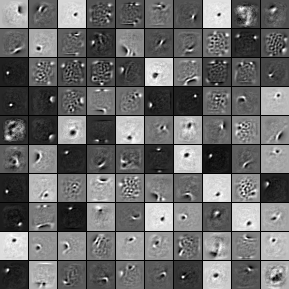
\includegraphics[width=.7\linewidth]{Images/Regularisation/decay_lamda0001.png}
% 						\caption{Untied weights with $\lambda=0.0001$}
% 						\label{fig:tied no reg}
% 					\end{center}
% 				\end{subfigure}
% 				\begin{subfigure}{.45\textwidth}
% 					\begin{center}
% 						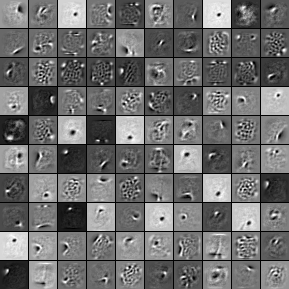
\includegraphics[width=.7\linewidth]{Images/Regularisation/tied_lamda0001.png}
% 						\caption{Tied weights with $\lambda=0.0001$}
% 						\label{fig:untied no reg}
% 					\end{center}
% 				\end{subfigure}
% 				\caption[An auto-encoder with tied weights]{100 randomly selected sub-representations in the hidden layer of auto-encoders trained without and with tied weights. One can notice that the tied weights do not have much influence on the representation learned. They are not a strong regularization method but they have the advantage to greatly reduce the parameter space. (see ~\ref{seq:Regularization methods for Auto-encoders/weight decay:} for explanations on $\lambda$)}
% 				\label{fig:Tied weight autoencoder}
% 			\end{center}
% 		\end{figure}
% 		
% 		
% 	\section{The weight decay:}
% 		\label{seq:Regularization methods for Auto-encoders/weight decay:}
% 		Weight decay is the name given to an $L_{2}$-regularization applied to auto-encoders. When the weight decay is applied the cost function becomes:
% 		
% 		\begin{equation}
% 			J_{wd} = J + \frac{\lambda}{2} \sum_{l=1}^{d-1}{\sum_{i=1}^{s_{l}}{\sum_{j=1}^{s_{l+1}}{\left(W_{ij}^{(l)}\right)^{2}}}}
% 		\end{equation}\\
% 		
% 		The relative importance given to the regularization term over the cost function is controlled by the parameter $\lambda$, called the \Important{weight decay}. This regularization tends to decrease the magnitude of the weights and helps prevent over-fitting. Here again, the idea is to prevent our machine from learning ill-shaped solutions where the encoding weights would be very small while the decoding ones would be large, as such solutions are very likely to over-fit the training set. Finally, one could notice that the weight decay is not applied to the bias. Indeed it usually makes no different to include it in the regularization \cite{Ng_course}.\\\par
% 		
% 		\begin{figure}[H]
% 			\begin{center}
% 				\begin{subfigure}{.45\textwidth}
% 					\begin{center}
% 						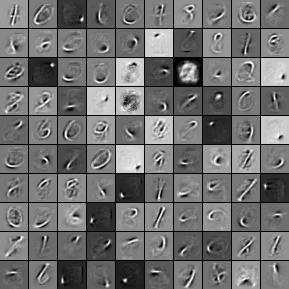
\includegraphics[width=.7\linewidth]{Images/Regularisation/no_reg.png}
% 						\caption{No regularization}
% 						\label{fig:decay no regularization}
% 					\end{center}
% 				\end{subfigure}
% 				\begin{subfigure}{.45\textwidth}
% 					\begin{center}
% 						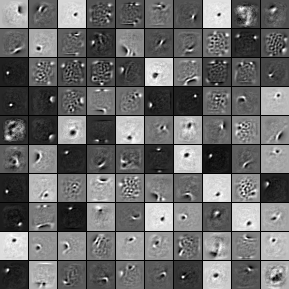
\includegraphics[width=.7\linewidth]{Images/Regularisation/decay_lamda0001.png}
% 						\caption{$\lambda=0.0001$}
% 						\label{fig:decay lambda 0.0001}
% 					\end{center}
% 				\end{subfigure}
% 				\caption[An auto-encoder with weight decay]{100 randomly selected sub-representations in the hidden layer of an auto-encoders trained with weight decay. One can notice that the representation learned without regularization is closer to what is consider as over-fitting (visible shapes of numbers); while the auto-encoder with weight decay learns smaller piece of elements of the training images (edges...). However, we have empirically noticed, that this regularization does not seem strong enough to constrain efficiently the learning alone.}
% 				\label{fig:weight decay autoencoder}
% 			\end{center}
% 		\end{figure}
% 
% 		
% 	\section{Sparse Auto-Encoders:}
% 		\label{seq:Regularization methods for Auto-encoders/Sparsity:}
% 		
% 		The sparsity is a regularization method that affects the hidden units. Informally, let us say that a neuron is ``active'' if its output value is ``close to'' the maximum value of the activation function (e.g.: 1 for a sigmoid), whereas it is ``inactive'' when its output value is ``close to'' the minimum value of the activation function (e.g.: -1 for the hyperbolic tangent). Then \Important{the sparsity constrain the neurons to be inactive most of the time}.\\\par
% 		
% 		More formally, let us compute the average activation of the hidden unit j over the training set:
% 		
% 		\begin{equation}
% 			\hat{\rho}_{j} = \frac{1}{m} \sum_{i=1}^{m}{\left[a_{1,j}(x_{i})\right]}
% 			\label{eq:Average activation}
% 		\end{equation}\\
% 		
% 		Where $a_{1,j}$ is the $j-th$ coordinate of the activation of the hidden unit $a_{1}$. Hence, the goal of the sparsity is to enforce the constraint:
% 		
% 		\begin{equation}
% 			\hat{\rho}_{j} = \rho
% 		\end{equation}\\
% 
% 		Where $\rho$ is the \Important{sparsity parameter}, and typically as a value close to zero. In other words, we would like the average activation of each hidden unit to be close to a pre-selected value close to zero. In order to satisfy this constraint, the hidden unit's activations values must mostly be near 0 across the training examples. Theoretically \Important{they would be activated only to encode one important characteristic in the input}.\\\par
% 		
% 		To achieve this, a penalty term that penalizes $\hat{\rho}_{j}$ from deviating significantly from $\rho$ have to be added to the objective function. Several choices are possible to ensure this, but the most widely used one is the Kullback-Leibler $\text{KL}(\rho \parallel \hat{\rho}_{j})$  divergence between a Bernoulli random variable with mean $\rho$ and a Bernoulli random variable with mean $\hat{\rho}_{j}$.
% 
% 		\begin{figure}[H]
% 			\begin{center}
% 				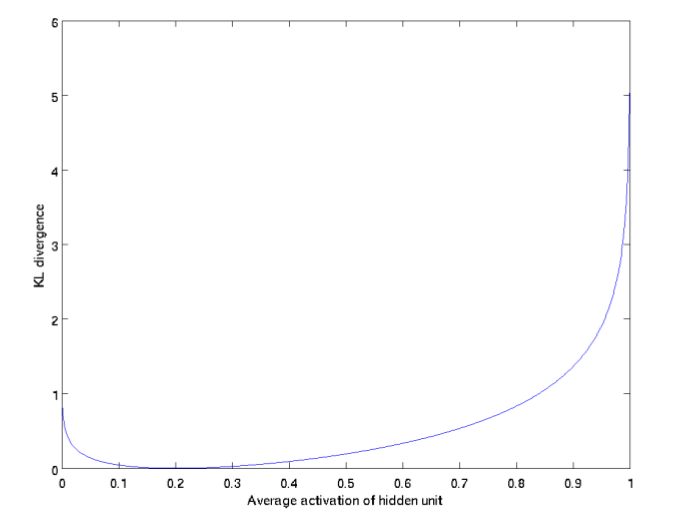
\includegraphics[width=3.5in]{Images/AE_SAE/KL_divergence.png}
% 				\caption[The Kullback-Leibler divergence]{Kullback-Leibler divergence for an objective distribution with a mean $\rho=0.2$}
% 				\label{fig:KL_divergence}
% 			\end{center}
% 		\end{figure}
% 		
% 		The KL-divergence is a standard function for measuring how different are two distributions. As display on the figure~\ref{fig:KL_divergence},
% 		its minimum is $0$ for $\rho = \hat{\rho}_{j}$, and then increase exponentially as $\hat{\rho}_{j}$ gets ``further'' from $\rho$. Thus, minimizing a penalty term based on this divergence has the effect of causing $\hat{\rho}_{j}$ to get close to $\rho$.\\\par
% 		
% 		The cost function when sparsity is applied becomes:
% 		
% 		\begin{equation}
% 			\begin{split}
% 				J_{sparse}	&= J + \beta \sum_{j=1}^{n_{1}}{\text{KL}(\rho \parallel \hat{\rho}_{j})} \\
% 										&= J + \beta \sum_{j=1}^{n_{1}}{\left(\rho \log \frac{\rho}{\hat{\rho}_{j}} + (1 - \rho) \log \frac{1 - \rho}{1 - \hat{\rho}_{j}}\right)}
% 			\end{split}
% 			\label{eq:Cost function with sparsity}
% 		\end{equation}\\
% 		
% 		Where $\beta$ controls the relative importance of the sparsity term over the cost function $J$.\\\par
% 		
% 		It is not obvious from the expression~\ref{eq:Average activation} but $\hat{\rho}_{j}$ depends on $\mathbf{W_{1}}$ and $b_{1}$. Hence, the KL-divergence term as to be incorporated into the cost derivative calculation. Luckily, there is a trick, involving only a small change the to backpropagation codes to include the sparsity term to it. The formula~\ref{eq:last layer error for backpropagation} to backpropagate the error has to be changed for the output layer in:
% 		
% 		\begin{equation}
% 			\delta^{(d)} = \frac{\partial }{\partial \mathbf{z^{(l)}}} J(\mathbf{x_{k}},y_{k}) + \beta \left(-\frac{\rho}{\hat{\rho}} + \frac{1- \rho}{1 - \hat{\rho}} \right)
% 			\label{eq:last layer error for backpropagation with sparsity}
% 		\end{equation}\\
% 
% 		One of the consequence is that $\hat{\rho}_{j}$ now has to be known to compute this term. Thus, it is necessary to compute a forward pass on all the training set first in order to compute the average activations on all the examples before computing the backpropagation on any example. This can be problematic when the dataset considered is too large to fit in the computer memory. In that case the forward pass will have to be done twice, first to compute $\hat{\rho}_{j}$ but as the results could not be stored a second forward pass will be necessary to compute the backpropagation, making the training computationally less efficient.\\
% 		
% 		\begin{figure}[H]
% 			\begin{center}
% 				\begin{subfigure}{.45\textwidth}
% 					\begin{center}
% 						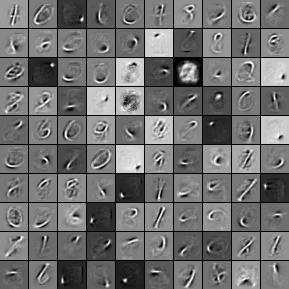
\includegraphics[width=.7\linewidth]{Images/Regularisation/no_reg.png}
% 						\caption{No regularization}
% 						\label{fig:sparsity no regularization}
% 					\end{center}
% 				\end{subfigure}
% 				\begin{subfigure}{.45\textwidth}
% 					\begin{center}
% 						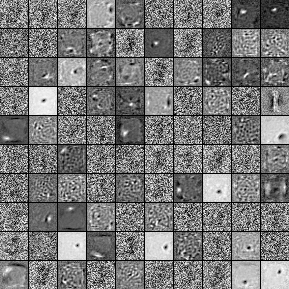
\includegraphics[width=.7\linewidth]{Images/Regularisation/sparsity_beta05_rho01.png}
% 						\caption{$\beta=0.1$ and $\rho=0.01$}
% 						\label{fig:sparsity beta0.1 rho0.01}
% 					\end{center}
% 				\end{subfigure}
% 				\caption[A sparse auto-encoder]{100 randomly selected sub-representations in the hidden layer of a sparse auto-encoders. Again one can notice that the representation learned without regularization is closer to what is consider as over-fitting (visible shapes of numbers); while the sparse auto-encoder learns smaller elements of the training images (edges...). Some cells of the sparse auto-encoder are still not trained (i.e.: looks like white noise) probably because the training set was to small to train them efficiently.}
% 				\label{fig:sparse autoencoder}
% 			\end{center}
% 		\end{figure}
% 
% 		
% 	\section{Contractive Auto-Encoders:}
% 		\label{seq:Regularization methods for Auto-encoders/Contractive:}
% 		
% 		The \Important{contractive penalization} \cite{Rifai_2011} is a penalty term which encourages the intermediate representation of the input to be \Important{robust to small changes around the training examples} (i.e.: that favors mappings that are more strongly contracting at the training samples). To encourage the robustness of the representation $f(x)$, the contractive penalty proposed to penalize its \Important{sensitivity} to a training example $\mathbf{x}$. This can be measured by the Frobenius norm of the Jacobian matrix $J_{f}(x)$ of the encoding.\\\par
% 			
% 		More formally, if an input $x \in \mathbb{R}^{n_{0}}$ is mapped by the encoding module $f$ to a representation $h(x) \in \mathbb{R}^{n_{1}}$, the sensitivity penalization term is the sum of squares of all partial derivatives of the extracted features with respect to the input dimensions:
% 			
% 		\begin{equation}
% 			\|J_{f}(x)\|_{F}^{2} = \sum_{i,j}{\left(\frac{\partial h_{j}(x)}{\partial x_{i}}\right)^{2}} 
% 		\end{equation}\\
% 			
% 		This penalization will force the representation in having low valued first derivatives, which will lead to an invariance or robustness of this representation for small variations of the input (i.e.: no steep changes). The cost function when for a \Important{contractive auto-encoder} becomes:
% 			
% 		\begin{equation}
% 			\begin{split}
% 				J_{CAE}	&= J + \delta \sum_{x \in \mathcal{D}_{train}}{\|J_{f}(x)\|_{F}^{2}} \\
% 										&= J + \delta \sum_{x \in \mathcal{D}_{train}}{\sum_{i,j}{\left(\frac{\partial h_{j}(x)}{\partial x_{i}}\right)^{2}}} \\
% 			\end{split}
% 			\label{eq:Cost function for a CAE}
% 		\end{equation}\\	
% 			
% 		While such a Jacobian term used alone would encourage a mapping to a useless constant representation, it is counterbalanced in auto-encoder training by the need for the learned representation to allow a good reconstruction of the input. The parameter $\delta$ control the relative importance of the contractive regularization over the simple cost function.\\
% 		
% 		\begin{figure}[H]
% 			\begin{center}
% 				\begin{subfigure}{.45\textwidth}
% 					\begin{center}
% 						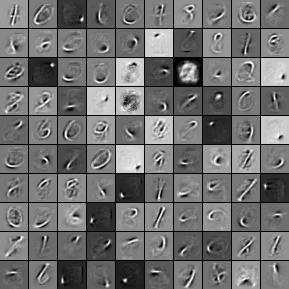
\includegraphics[width=.7\linewidth]{Images/Regularisation/no_reg.png}
% 						\caption{No regularization}
% 						\label{fig:contractive no reg}
% 					\end{center}
% 				\end{subfigure}
% 				\begin{subfigure}{.45\textwidth}
% 					\begin{center}
% 						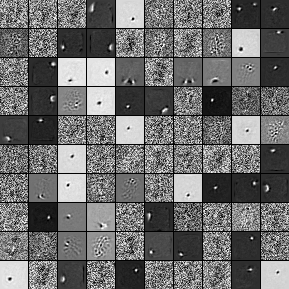
\includegraphics[width=.7\linewidth]{Images/Regularisation/cont_delta01.png}
% 						\caption{$\delta=0.1$}
% 						\label{fig:contractive delta0.1}
% 					\end{center}
% 				\end{subfigure}
% 				\caption[A contractive auto-encoder]{100 randomly selected sub-representations in the hidden layer of a contractive auto-encoders. Again one can notice that the representation learned without regularization is closer to what is consider as over-fitting (visible shapes of numbers); while the contractive auto-encoder learns smaller elements of the training images (edges...). Compared to the sparse auto-encoder, the contractive one seems to provide a more stable solution (i.e.: the representation is more net). Again some cells of the contractive auto-encoder are still not trained (i.e.: looks like white noise) probability because the training set was to small to train them efficiently.}
% 				\label{fig:contractive autoencoder}
% 			\end{center}
% 		\end{figure}
% 	
% 	
% 	\section{Dropout noise:}
% 		\label{seq:Regularization methods for Auto-encoders/Dropout:}
% 
% 		The \Important{dropout noise} falls into the broader category of learning methods that artificially corrupt training data to stabilize predictions. Even if the link between the feature corruption and regularization has been intensively studied \cite{Matsuoka_1992, Bishop_1995, Rifai_2011b}, the theoretical foundations of the success of the dropout noise for deep neural network are yet to be completely understand.\\\par
% 		
% 		The idea behind the dropout noise is to prevent over-fitting by \Important{randomly omitting part of the features (i.e.: connections) on each training example} \cite{Hinton_2012}. In his procedure Hinton drops up to $50\%$ of the connections. This prevents complex co-adaptations in which a feature detector is only helpful in the context of several other specific feature detectors. Instead, each neuron learns to detect a feature that is generally helpful for producing the correct answer given the combinatorially large variety of internal contexts in which it must operates.\\\par
% 		
% 		\begin{figure}[H]
% 			\begin{center}
% 				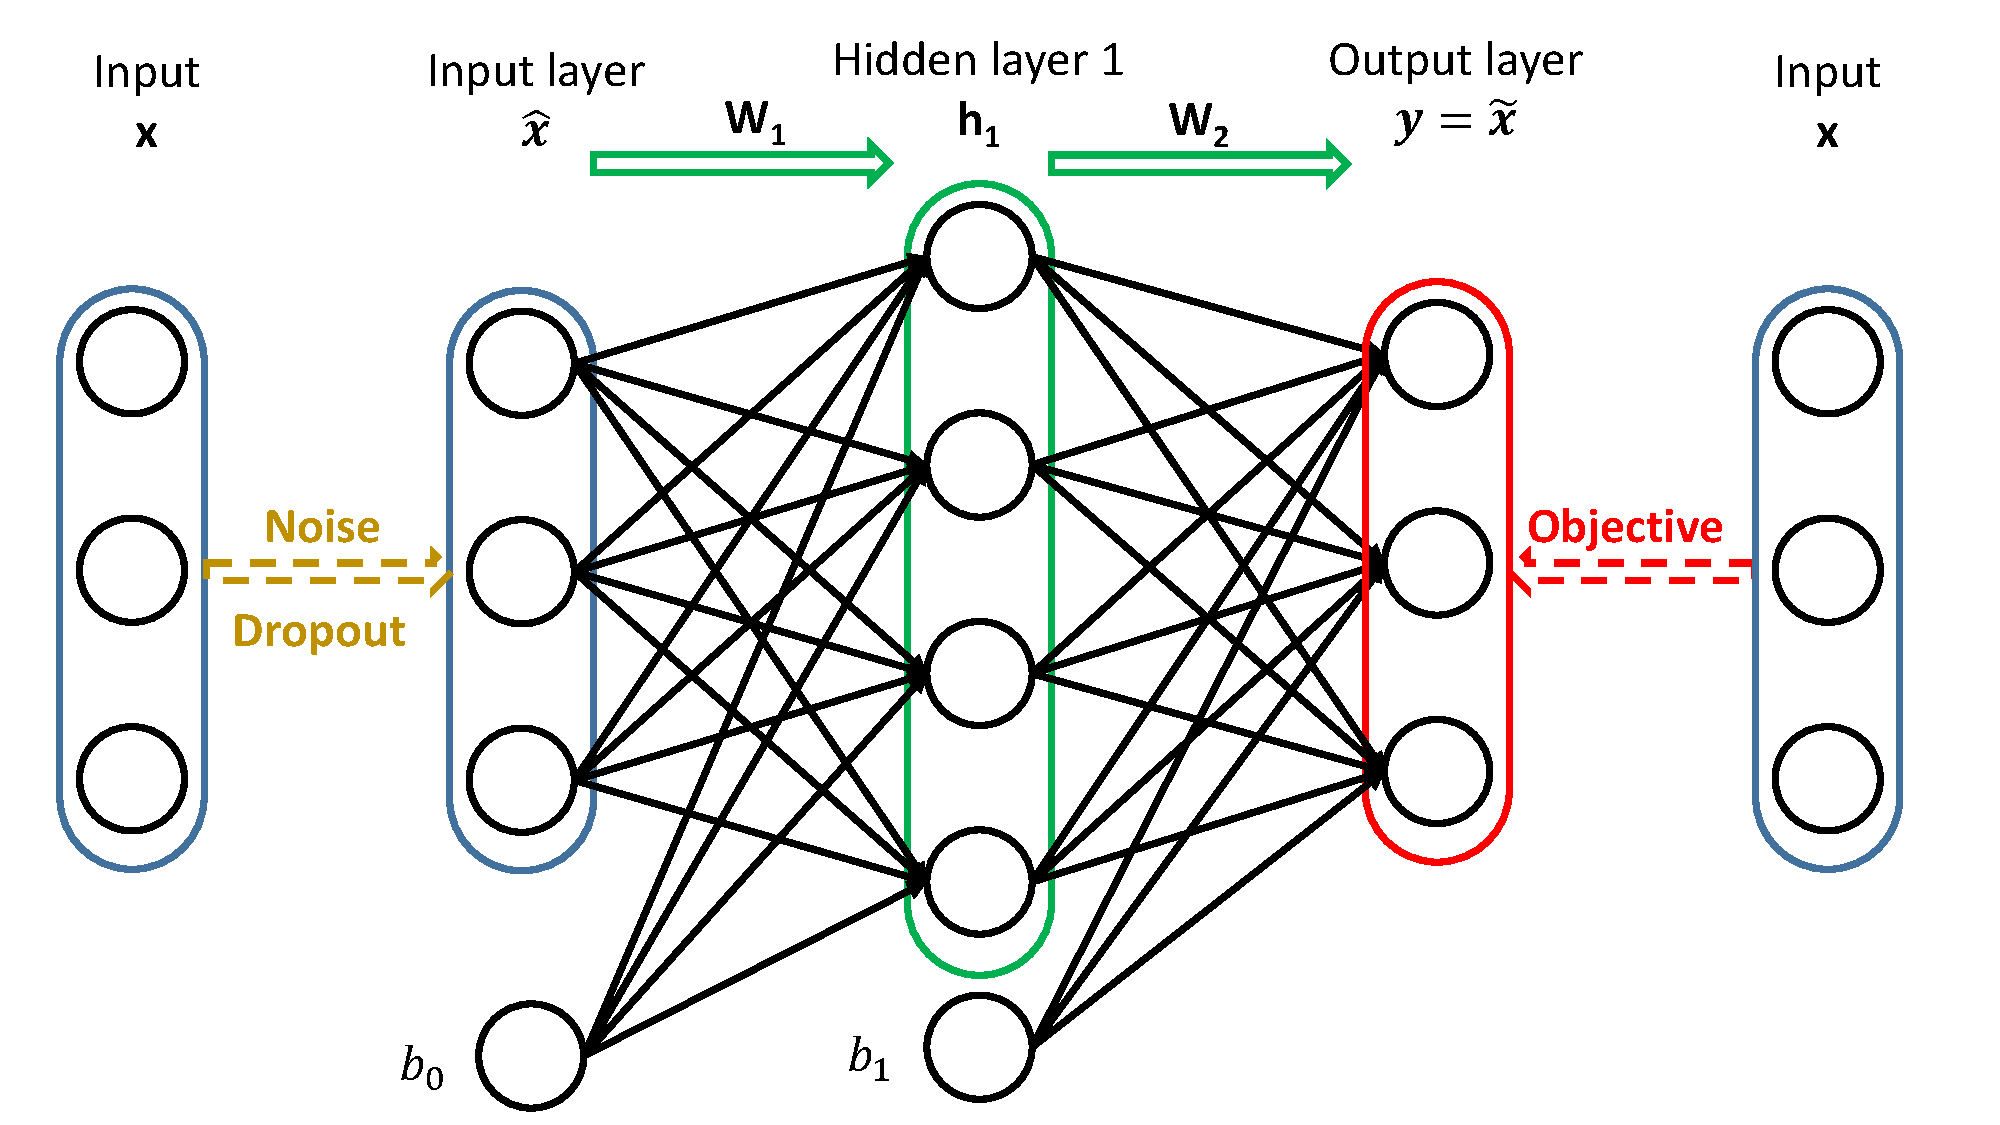
\includegraphics[width=3.5in]{Images/Regularisation/train_with_noise.pdf}
% 				\caption{Training with noise or dropout procedure}
% 				\label{fig:train_with_noise}
% 			\end{center}
% 		\end{figure}
% 		
% 		\begin{figure}[H]
% 			\begin{center}
% 				\begin{subfigure}{.45\textwidth}
% 					\begin{center}
% 						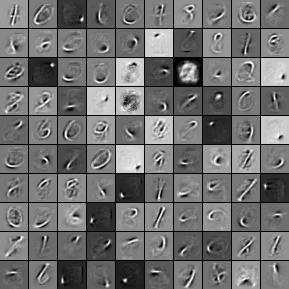
\includegraphics[width=.7\linewidth]{Images/Regularisation/no_reg.png}
% 						\caption{No regularization}
% 						\label{fig:noise no reg}
% 					\end{center}
% 				\end{subfigure}
% 				\begin{subfigure}{.45\textwidth}
% 					\begin{center}
% 						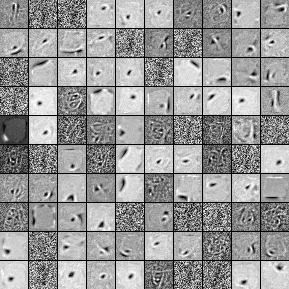
\includegraphics[width=.7\linewidth]{Images/Regularisation/drop_masking05.png}
% 						\caption{Dropout rate of $50\%$}
% 						\label{fig:noise0.5}
% 					\end{center}
% 				\end{subfigure}
% 				\caption[An auto-encoder with dropout]{100 randomly selected sub-representations in the hidden layer of auto-encoders trained with $50\%$ dropout. Again one can notice that the representation learned without regularization is closer to what is consider as over-fitting (visible shapes of numbers); while the auto-encoder trained with dropout learns smaller elements of the training images (edges...). Compared to the contractive auto-encoder, the auto-encoder trained with dropout seems to have use more neurons but learned slightly less stable representation (i.e.: less net).}
% 				\label{fig:Dropout autoencoder}
% 			\end{center}
% 		\end{figure}
% 		
% 		
% 		\section{Combined regularizations:}
% 		One could imagine to train an auto-encoder using more than one regularization method. This approach has the disadvantage to complicate greatly the optimization problem to be solved during the unsupervised learning phase. Indeed, the objective function to be minimized when using several regularization methods is highly non-regular with regard to the network weights.\\
% 		
% 		\begin{equation}
% 			J_{comb} = J	+ \delta \sum_{x \in \mathcal{D}_{train}}{\|J_{f}(x)\|_{F}^{2}} 
% 										+ \beta \sum_{j=1}^{n_{1}}{\text{KL}(\rho \parallel \hat{\rho}_{j})} 
% 										+ \frac{\lambda}{2} \sum_{l=1}^{n_{l}-1}{\sum_{i=1}^{s_{l}}{\sum_{j=1}^{s_{l+1}}{\left(W_{ij}^{(l)}\right)^{2}}}}
% 			\label{eq:Cost function for a combine regularization}
% 		\end{equation}\\
% 		
% 		However when the learning algorithm converges effectively the representations learned are of very good quality.
% 		
% 		\begin{figure}[H]
% 			\begin{center}
% 				\begin{subfigure}{.45\textwidth}
% 					\begin{center}
% 						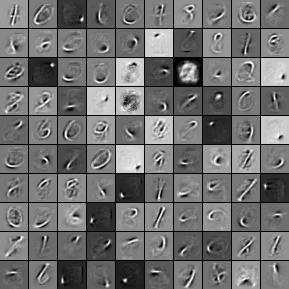
\includegraphics[width=.7\linewidth]{Images/Regularisation/no_reg.png}
% 						\caption{No regularization}
% 						\label{fig:combine no reg}
% 					\end{center}
% 				\end{subfigure}
% 				\begin{subfigure}{.45\textwidth}
% 					\begin{center}
% 						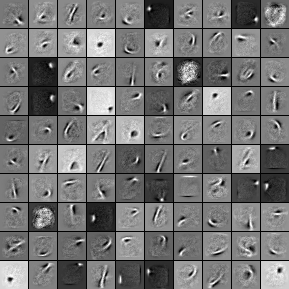
\includegraphics[width=.7\linewidth]{Images/Regularisation/combine.png}
% 						\caption{All the regularization combine}
% 						\label{fig:combine}
% 					\end{center}
% 				\end{subfigure}
% 				\caption[An auto-encoder with combined regularizations]{100 randomly selected sub-representations in the hidden layer of auto-encoders trained with $40\%$ dropout, a weight decay $\lambda=0.0001$, a sparsity coefficients of $\beta=0.3$ and $\rho=0.1$, a contractive coefficient $\delta=0.1$ and tied weights.}
% 				\label{fig:Combined regularization autoencoder}
% 			\end{center}
% 		\end{figure}
% 	
% 		
% %%%%%%%%%%%%%%%%%%%%%%%%%%%%%%%%%%%%%%%%%%%%%%%%%%%%%%%%%%%%%%%%%%%%%%%%%%%%%%%%%%%%%%%%%%%%%%%%%%%%%%%%%%%%%%%%%%%%%%%%%%%%%%%%%%%%%%%%%%%%%%%%%%%%
% \chapter{Implementation of the Stack Auto-Encoder:}
% 	\label{chap:Implementation of the SAE:}
% 	The implementation of the SAEs can be spited in two steps. First the implementation on an \Important{object Auto-Encoder} with all the methods necessary for its unsupervised training and assessing its performances. The second step is the implementation of an \Important{object Stack Auto-Encoder} having all the methods necessary to perform the piling of the auto-encoder and perform the SAE's unsupervised pre-training as well as the supervised fine tuning.	
% 	
% 	
% 	\section{GPU computing and Theano:}
% 		\label{seq:Implementation of the SAE/GPU computing and Theano:}
% 		For simplicity reasons, we have decided to implement the SAEs using \Important{Python 2.7.3}. But if one implements a deep neural network using only usual python's library (i.e.: numpy, scipy...), the mono-threaded CPU computed neural network will appears to be very slow to train. Indeed DNNs are massively parallel structures with up to millions of parameters. For example, one of the deep neural network performing the best on the MNIST dataset \cite{LeCun_webPage} has 6 layers with respectively 784, 2500, 2000, 1500, 1000, 500 and 10 units. With such an architecture and advanced regularization methods the error rate on the test set is of only $0.35\%$. But those excellent performances have a cost as this network has about $20\,930\,000$ parameters\footnote{$20\,930\,000= 784 \times 2\,500 + 2\,500 \times 1\,500 + 1\,500 \times 1\,000 + 1\,000 \times 500 + 500 \times 10$.\\ Only the weights connecting the layers have been include in the ``number of parameters computation'' but the actual number of 
% parameters must be higher due to meta-parameters (regularization coefficients, learning rates...)} to be optimized. Moreover, beside the number of unit itself, a deep neural network is composed of thousands or more identical units which perform the same computation on different data.  Most of these units have no data interdependency, and can thus can be computed simultaneously. Training such a network is difficult on normal CPUs because during training phase there are a lot of data communications between the units. Luckily most of the time the entire network can be put on a single GPU instead of CPUs and it greatly speeds up the training process. Hence, the communication latency is reduced, the bandwidth is increased, and the size and power consumption are significantly decreased. For example one of the simplest but also the best training algorithms, Stochastic Gradient Descent, can \Important{run up to 40 times faster on a GPU as compared to a CPU} \cite{Theano}.\\\par
% 		
% 		Aware of this issue, we have decided to use the python library \Important{Theano} \cite{Theano} to implement the SAEs. Theano is a library wrapping CUDA (i.e.: GPU programing language) code for Python and allowing a simple access and control over the GPUs. Beside simplifying the usage of GPUs for calculations, Theano also allows \Important{symbolic calculus} (i.e.: let you to define, optimize, and evaluate mathematical expressions and is specially designed for those involving multi-dimensional arrays -numpy.ndarray). This feature is useful for neural network as some operations such as the gradient computation for example does not have to be hard coded anymore. The expression of the gradient is automatically computed once, and then its value is evaluated for each instance (instead of computing a hard coded gradient formula for every single instance).
% 		
% 		
% 	\section{Auto-Encoder:}
% 		\label{seq:Implementation of the SAE/AE:}
% 		In our implementation, the auto-encoder is a python object that has to be able to perform the unsupervised training procedure described in the section~\ref{seq:AE and SAE/Training procedure:}. To do so the AE object has to:\\
% 		
% 		\begin{itemize}
% 			\item \Important{Receive} an architecture, and create the corresponding network. In this case, the architecture is the number of input units, the number of unit in the representation layer, what are the activation functions used in the representation layer and in the output layer, and eventually a value for the network's weights initialization.\\
% 			
% 			\item \Important{Be able to} perform the unsupervised training procedure (section~\ref{seq:AE and SAE/Training procedure:}) given an unlabeled dataset and regularization parameters.\\
% 			
% 			\item \Important{Be able to} provide with an evaluation of the performances of the AE (i.e.: reconstruction error) and -if relevant- a visualization of the learned representation.\\
% 			
% 			\item \Important{Be able to} encode and decode data.\\
% 		\end{itemize}
% 
% 		Given those specifications, the UML diagram of the implemented auto-encoder object is given in figure~\ref{fig:AE_uml}.\\
% 
% 		\begin{figure}[H]
% 			\begin{center}
% 				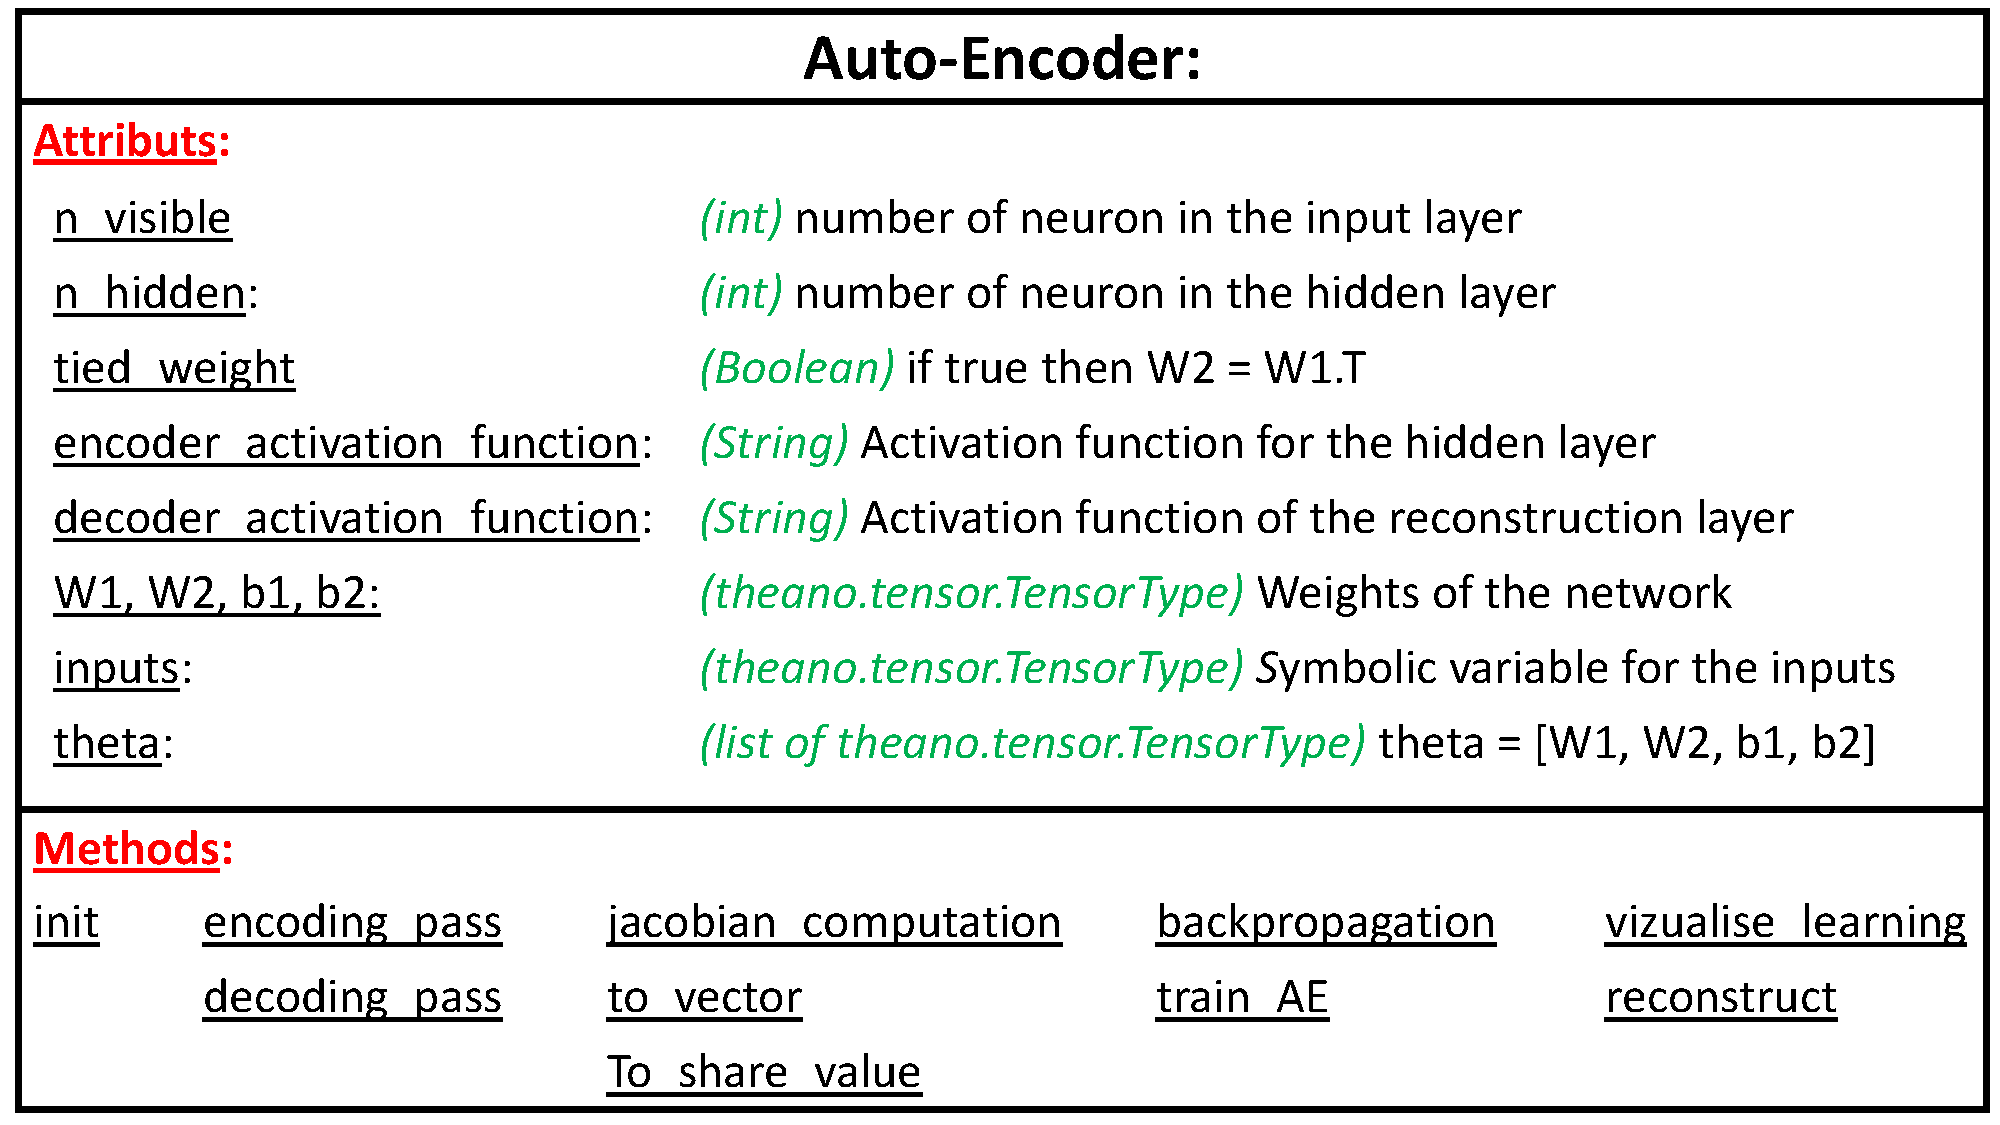
\includegraphics[width=5in]{Images/Implementation/AE_uml.pdf}
% 				\caption{The UML diagram of the object Auto-Encoder}
% 				\label{fig:AE_uml}
% 			\end{center}
% 		\end{figure}
% 		
% 		
% 	\section{Stack Auto-Encoder:}
% 		\label{seq:Implementation of the SAE/SAE:}
% 		In our implementation, the stack auto-encoder is a python object that has to able to perform the stacking and the training procedure described in the section~\ref{seq:AE and SAE/SAE:}. To do so the SAE object has to:\\
% 		
% 		\begin{itemize}
% 			\item \Important{Receive} an architecture, and create the corresponding network. In this case, the architecture is a list of architectures of AEs (section~\ref{seq:Implementation of the SAE/AE:}).\\
% 			
% 			\item \Important{Be able to} perform the greedy-layer wise unsupervised training procedure given an unlabeled dataset and regularization parameters.\\
% 			
% 			\item \Important{Be able to} perform the supervised fine tuning procedure given a labeled dataset and learning meta-parameters.\\
% 			
% 			\item \Important{Be able to} use the representation learned during the unsupervised phase as a feature generator to feed an independent classifier/regressor.\\
% 			
% 			\item \Important{Be able to} provide with an evaluation of the performances of the SAE (i.e.: reconstruction error) and -if relevant- a visualization of the learned representations.\\
% 			
% 			\item \Important{Be able to} encode and decode data.\\
% 			
% 			\item \Important{Be able to} save the trained model.\\
% 		\end{itemize}
% 
% 		Given those specifications, the UML diagram of the implemented stack auto-encoder object is given in figure~\ref{fig:SAE_uml}.\\
% 	
% 		\begin{figure}[H]
% 			\begin{center}
% 				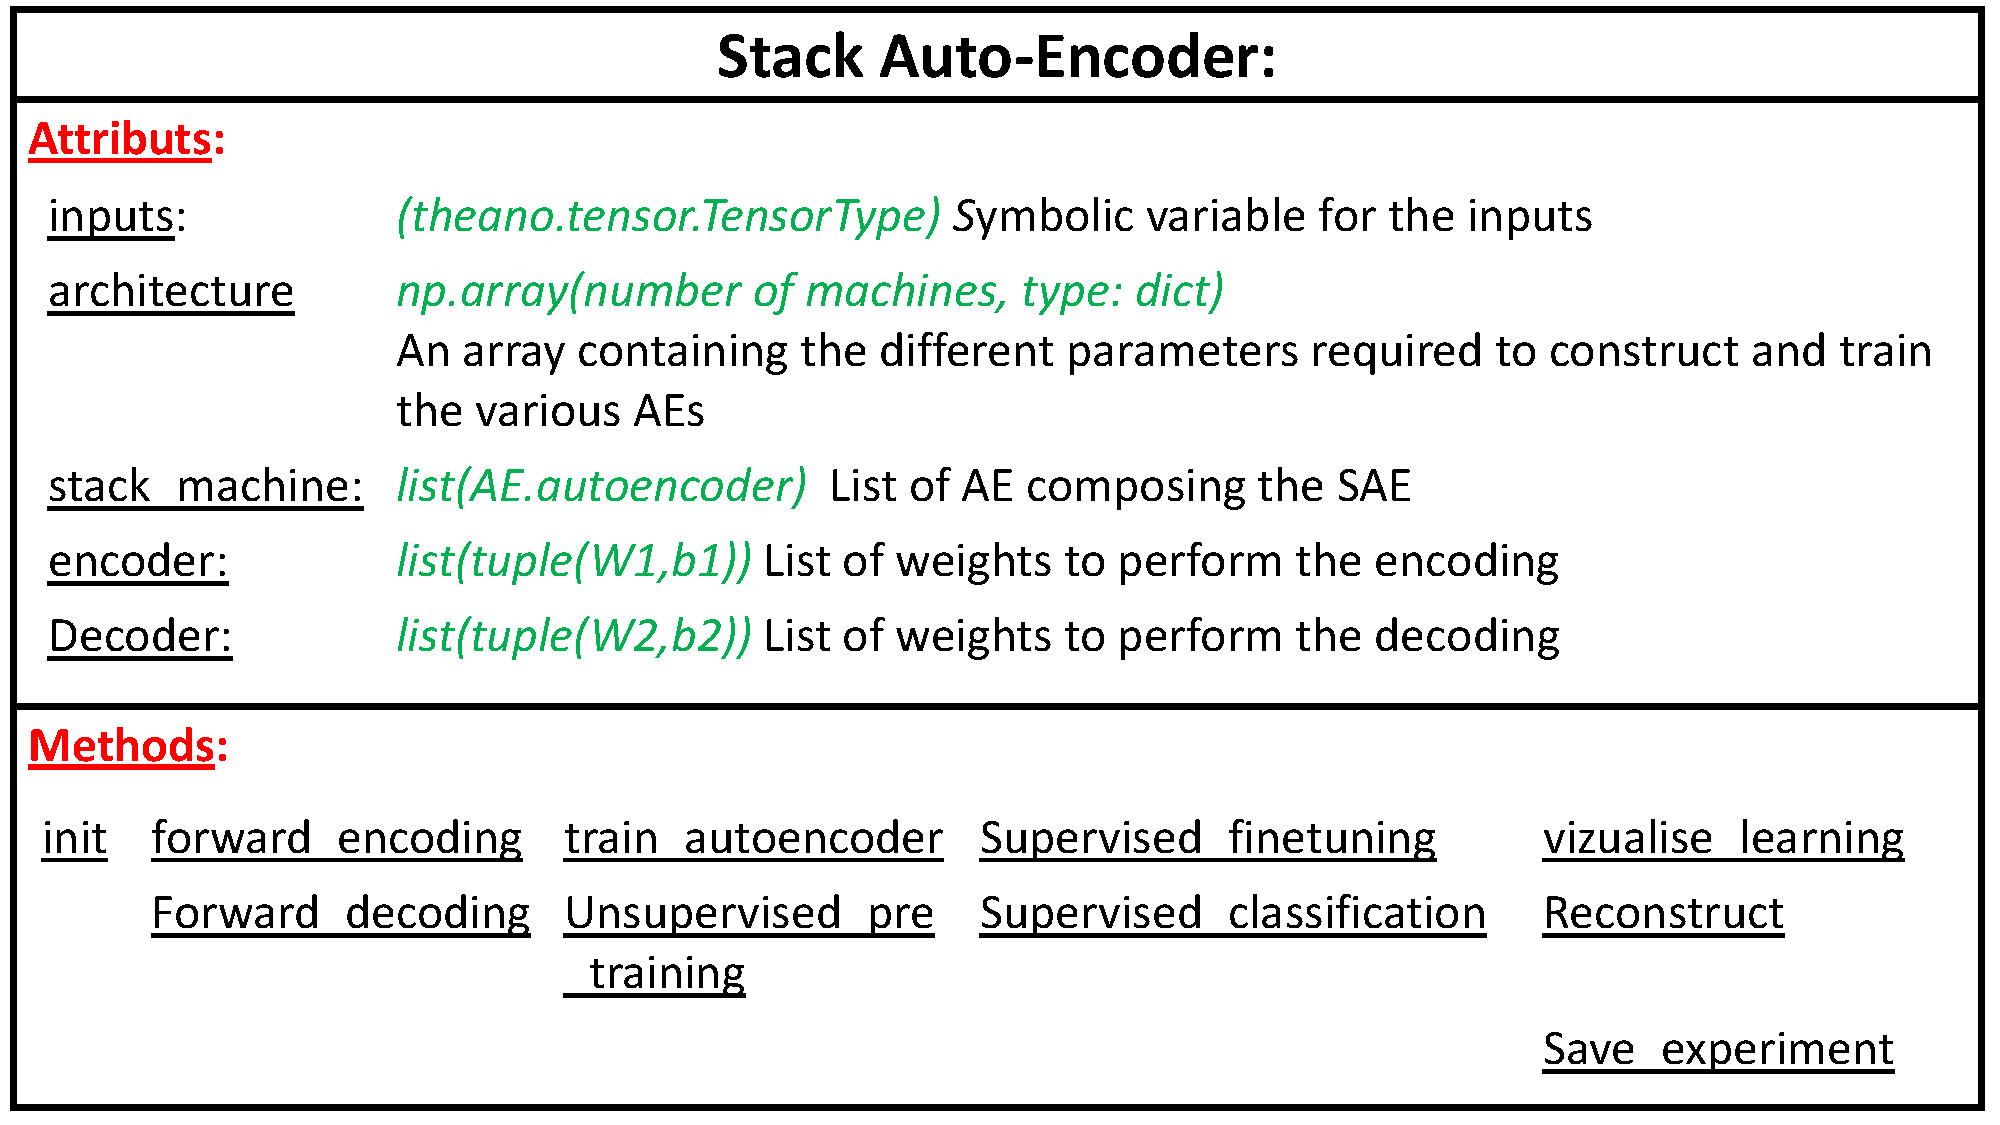
\includegraphics[width=5in]{Images/Implementation/SAE_uml.pdf}
% 				\caption{The UML diagram of the object Stack Auto-Encoder}
% 				\label{fig:SAE_uml}
% 			\end{center}
% 		\end{figure}


%%%%%%%%%%%%%%%%%%%%%%%%%%%%%%%%%%%%%%%%%%%%%%%%%%%%%%%%%%%%%%%%%%%%%%%%%%%%%%%%%%%%%%%%%%%%%%%%%%%%%%%%%%%%%%%%%%%%%%%%%%%%%%%%%%%%%%%%%%%%%%%%%%%%
\chapter{Experimental results:}
	\label{chap:Experimental results}
	
	The aim of this internship was to implement our own deep neural networks and then test it on several datasets. We first decided to test them on MNIST(section~\ref{seq:Experimental results/MNIST:} -\cite{LeCun_webPage}) as it is one of the most widely used dataset in the literature on deep neural network. Then we assessed the performances of a deep neural network used as a feature generator in a Kaggle competition (section~\ref{seq:Experimental results/kaggle:} -\cite{Kaggle_higgs}).
	
	
	\section{MNIST:}
		\label{seq:Experimental results/MNIST:}
		MNIST is a dataset of labeled \Important{handwritten gray scale digits}. It has a training set of $60\,000$ examples, and a test set of $10\,000$ examples. The input images have $28 \times 28$ pixels (i.e.: 784 dimensions) an a small pre-processing have been done, as the digits are size-normalized, centered in a fixed-size image and the pixel values have been shifted between 0 and 1.\\\par

		The advantage with an image dataset is the possibility to plot the representations learned by the network in order to have an idea of the quality of the features learned. But this method is not $100\%$ accurate as what a human may considerate as a ``good'' intermediate representation may not be the best one for a computer. Despite this, we used this visual argument as well as the classification error to assess the performances of the stack auto-encoders on MNIST.\\\par
		
		As the parameter space to be tested is really rich, we decided to restrain to a few number of architectures for the network (3 hidden layers of $500$ units, 3 hidden layers of $1\,000$ units and 4 layers with respectively $1\,000$, $500$, $100$ and $20$ units). So far our best classification error on the validation set is around $1.1\%$ which is good but still far above the current state of the art for deep neural networks \cite{LeCun_webPage}.\\\par
		
		MNIST was also useful to grasp the influence of each meta-parameters of the learning. We studied different learning rates, different regularizations. We also implemented the \Important{second order gradient descent algorithm L-BFGS} to try to improve the quality of the learning and so improve our results. Some examples of the representations learned can be seen on the following figures.
		
		\begin{figure}[H]
			\begin{center}
				\begin{subfigure}{.7\textwidth}
					\begin{center}
						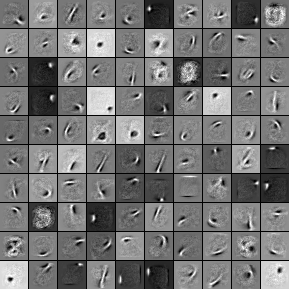
\includegraphics[width=.6\linewidth]{Images/Experience/3L500_all_layer_0.png}
						\caption{100 randomly selected sub-representations in the first hidden layer}
						\label{fig:500_layer0}
					\end{center}
				\end{subfigure}
				\begin{subfigure}{.7\textwidth}
					\begin{center}
						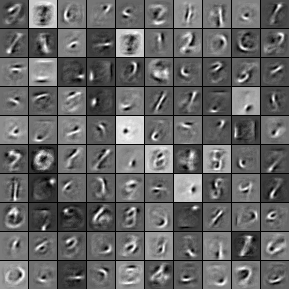
\includegraphics[width=.6\linewidth]{Images/Experience/3L500_all_layer_1.png}
						\caption{100 randomly selected sub-representations in the second hidden layer}
						\label{fig:500_layer1}
					\end{center}
				\end{subfigure}
				\begin{subfigure}{.7\textwidth}
					\begin{center}
						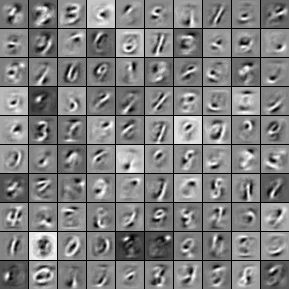
\includegraphics[width=.6\linewidth]{Images/Experience/3L500_all_layer_2.png}
						\caption{100 randomly selected sub-representations in the third hidden layer}
						\label{fig:500_layer2}
					\end{center}
				\end{subfigure}
				\caption[A 3 hidden layers 500-500-500 stack auto-encoder]{A 3 hidden layers 500-500-500 stack auto-encoder with the contractive penalization weighted to $\delta=0.1$, the sparsity to $\beta=0.1$ and $\rho=0.1$, the weight decay to $\lambda=0.0001$ and a dropout rate of $40\%$ and the auto-encoders' weights are tied. The cost function is the cross-entropy.}
				\label{fig:3L500_500_500}
			\end{center}
		\end{figure}
		
		\begin{figure}[H]
			\begin{center}
				\begin{subfigure}{.7\textwidth}
					\begin{center}
						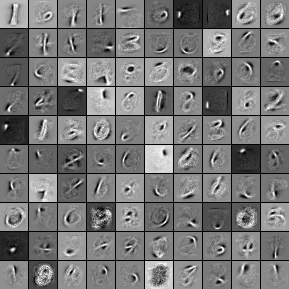
\includegraphics[width=.6\linewidth]{Images/Experience/3L1000_all_layer_0.png}
						\caption{100 randomly selected sub-representations in the first hidden layer}
						\label{fig:1000_layer0}
					\end{center}
				\end{subfigure}
				\begin{subfigure}{.7\textwidth}
					\begin{center}
						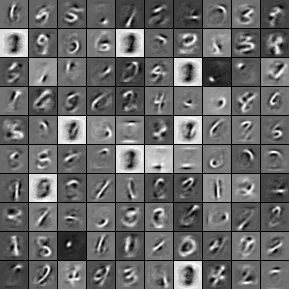
\includegraphics[width=.6\linewidth]{Images/Experience/3L1000_all_layer_1.png}
						\caption{100 randomly selected sub-representations in the second hidden layer}
						\label{fig:1000_layer1}
					\end{center}
				\end{subfigure}
				\begin{subfigure}{.7\textwidth}
					\begin{center}
						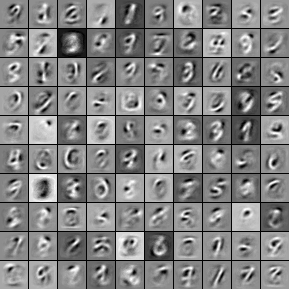
\includegraphics[width=.6\linewidth]{Images/Experience/3L1000_all_layer_2.png}
						\caption{100 randomly selected sub-representations in the third hidden layer}
						\label{fig:1000_layer2}
					\end{center}
				\end{subfigure}
				\caption[A 3 hidden layers 1000-1000-1000 stack auto-encoder]{A 3 hidden layers 1000-1000-1000 stack auto-encoder with the contractive penalization weighted to $\delta=0.1$, the sparsity to $\beta=0.1$ and $\rho=0.1$, the weight decay to $\lambda=0.0001$ and a dropout rate of $40\%$ and the auto-encoders' weights are tied. The cost function is the cross-entropy.}
				\label{fig:3L1000_1000_1000}
			\end{center}
		\end{figure}
		
		The two experiments whose results are introduced in figure~\ref{fig:3L500_500_500} and~\ref{fig:3L1000_1000_1000}, use the same regularization parameters but the second one have a network with twice as many hidden units. We visualize the weights connecting the layer to the previous one projected back into the input space. The first experiences is a stack auto-encoder with 3 hidden layers with 500 units each. As expected the deep network first learns low level features (figure~\ref{fig:500_layer0}: small parts of number, edges) and move to higher level features (figure~\ref{fig:500_layer2}: some numbers can be guessed). Even if the same general behavior can be witnessed for the second experiment (figure~\ref{fig:3L1000_1000_1000}) involving this time a stack auto-encoder with 3 hidden layers with $1\,000$ units each, one can notice that some of the unit display unidentified shapes (~\ref{fig:1000_layer1}: second row column 1 and 5 for example). This could be a sign that this network is too big to learn the 
ideal representation or that the regularization applied is not strong enough.   
		
		
	\section{Kaggle higgs competition:}
		\label{seq:Experimental results/kaggle:}
		
		Another goal of the internship was to assess the performances of the deep neural networks for exploratory data analyses. To do so we took a data science-like problem, where we have few or no idea on what is the meaning of each feature of the input vector. Our choice has been the dataset provided provided for the \Important{Kaggle Higgs Boson Challenge} \cite{Kaggle_higgs}. The contest is sponsored by the CERN and aim at analyzing the data collected in the Large Hadron Collider. The contestants are asked to classified the events (i.e.: instance of the dataset) between the ``signal'' and ``noise''.\\\par
		
		The usual procedure to tackle this kind of problems would be to manually transform the given features in order to find a more suitable representation space to perform the classification. But beside being time consuming, this is hard to do when, as here, the input's physical meanings are not easy to understand. However as we have seen in the section~\ref{seq:Deep neural networks/Advantages of a deep architecture}, the deep neural networks should allow to circumvent this issue by performing an unsupervised feature generation.\\\par

		Hence, the idea is to realize the unsupervised training of a stack auto-encoder on the train set and then use the representation of the dataset learned as an input for a classifier. In order to assess the gain in performances provide by the unsupervised feature generation we will compare to the same classifier trained on the raw input data. Unfortunately so far the results are not very good. Mainly because we have no other way to select an architecture for the network but to try it  and see to what performances it yield to, which is a slow process.		

%%%%%%%%%%%%%%%%%%%%%%%%%%%%%%%%%%%%%%%%%%%%%%%%%%
%%%%%%%%%%%%%%%%%%%%%%%%%%%%%%%%%%%%%%%%%%%%%%%%%%
\chapter{Conclusion:}
  \paragraph{Scattering hidden Markov tree:}
    The stack auto-encoders and more generally the deep neural networks are a very powerful tool as they allow to realize machine learning tasks with virtually no human prior or even intervention. However, we have seen during our experiments how hard to optimize where those deep architectures. Indeed the optimization process takes place at two very different levels.\\\par
    
    Given a fix architecture, making sure to find the network's parameters minimizing the error is still an open issue as the optimization problem to be solved is non-linear and involves many free parameters. Even if the unsupervised pre-training problem is supposed to be easier to solve, the \Important{effective minimization is still not certain} (see \cite{Xavier_2010} for more information on this topic).\\\par
    
    Another issue in the learning procedure is to control the over-fitting. Many regularization methods are available (see chapter~\ref{chap:Regularization methods for Auto-encoders}) and provide encouraging results. However, they also make the optimization problem tackled during the training phase harder to be solved. Thus \Important{a better understanding of the regularization for deep neural networks is required} in order to adapt the amount of regularization to the problem.\\\par
    
    Finally, there is also an open question on \Important{how to find the best architecture for the network given a problem}. Today the most widely used method remains a greed search on both the number of layers and the number of units. But such a process is time consuming, not very precise nor efficient. Many researchers are convinced that the next evolution in neural network is to create  networks with an adaptive architecture (see the ``next steps" section of \cite{Bengio_2009} for more information on the topic).\\\par
    
  \paragraph{Next steps:}
    This internship at IPAL has been very interesting. It has been a good opportunity to learn a lot more about machine learning in general, to acquire a good knowledge of the deep architecture and to apply the knowledge acquired from both Supélec and the internship to real world problems.\\\par
    
    It was also the perfect opportunity to discover and confirm my taste for the research environment.
    
    
%%%%%%%%%%%%%%%%%%%%%%%%%%%%%%%%%%%%%%%%%%%%%%%%%%
%%%%%%%%%%%%%%%%%%%%%%%%%%%%%%%%%%%%%%%%%%%%%%%%%%
\chapter{Acknowledgements:}

	First, I would like to thank my two supervisors Antoine and Oliver at IPAL for their advices as well as their support. I would also like to express my gratitude to Hanlin Guo for sharing his knowledge of deep learning and for all the tips he gave me.\\\par
	
	Second, this internship would not have be the same without the friendly atmosphere of the laboratory. That is why I would like to thanks all the other IPAL's interns as well as the PHD candidates.\\\par 
	
	Lastly, I would like to thank the IPAL laboratory for the high quality infrastructures and hardwares provided during the internship.
	
	
%%%%%%%%%%%%%%%%%%%%%%%%%%%%%%%%%%%%%%%%%%%%%%%%%%%%%%%%%%%%%%%%%%%%%%%%%%%%%%%%%%%%%%%%%%%%%%%%%%%%%%%%%%%%%%%%%%%%%%%%%%%%%%%%%%%%%%%%%%%%%%%%%%%%
%%%%%%%%%%%%%%%%   
% Bibliography %
%%%%%%%%%%%%%%%%
\begin{thebibliography}{99}
	
	\bibitem{Rosenblatt_1958} F. Rosenblatt: {\em The perceptron: A probabilistic model for information storage and organization in the brain}\\
	Psychological Review, 65:386 - 408, 1958.  
  
	\bibitem{LeCun_1985} Y. LeCun: {\em Une procédure d'apprentissage pour réseau à seuil asymmetrique} (A learning scheme for asymmetric threshold networks)\\
	In Cognitiva 85, pages 599 – 604, Paris, France. 1985.
  
	\bibitem{Rumelhart_1986} D. E. Rumelhart,G. E. Hinton and R. Williams: {\em Learning representations by back-propagating errors}\\
  Nature, 323:533 – 536, 1986.
  
	\bibitem{McCulloch_1943} W. McCulloch and W. Pitts: {\em A logical calculus of the ideas immanent in nervous activity}\\
	Bulletin of Mathematical Biophysics, 5:115 – 133, 1943.
	
	\bibitem{Cybenko_1989} G. Cybenko: {\em Approximations by superpositions of sigmoidal functions}\\
	Mathematics of Control, Signals, and Systems, 2(4):303 – 314, 1989.
  
	\bibitem{Hornik_1991} K. Hornik: {\em Approximation capabilities of multilayer feedforward networks}\\
	Neural Networks, 4(2):251–257, 1991.
  
	\bibitem{LeCun_webPage} Y. LeCun: {\em Personal web page gathering the results of various algorithms on the MNIST classification problem}\\
	\url{http://yann.lecun.com/exdb/mnist/}
  
	\bibitem{Bengio_2009} Y. Bengio: {\em Learning Deep Architecture for AI}\\
	Fondation and Trends in Machine Learning Vol. 2, No. 1 1 - 127, 2009.
  
	\bibitem{Freund_1996} Y. Freund and R. E. Schapire: {\em Experiments with a new boosting algorithm}\\
	Machine Learning: Proceedings of Thirteenth International Conference, p.148 - 156, USA: ACM, 1996.
  
	\bibitem{Serre_2007} T. Serre, G. Kreiman, M. Kouh, C. Cadieu, U. Knoblich and T.Poggio: {\em A quantitative theory of immediate visual recognition}\\
	Progress in Brain Research, Computational Neuroscience: Theoretical Insights into Brain Function, vol. 165, p.33 – 56, 2007.

	\bibitem{Hastad_1986} J. Hastad: {\em Almost Optimal Lower Bounds for Small Depth Circuits}\\
	STOC, 1986.
	
	\bibitem{Bengio_2007} Y. Bengio, P. Lamblin, D. Popovici and H. Larochelle: {\em Greedy layer-wise training of deep networks}\\
	Advances in Neural Information Processing Systems 19 (NIPS’06), (B. Schlkopf, J. Platt, and T. Hoffman, eds.), p.153 – 160, MIT Press, 2007.

	\bibitem{Geman_1984} S. Geman and D. Geman: {\em Stochastic relaxation, gibbs distributions, and the Bayesian restoration of images}\\
	IEEE Transactions on Pattern Analysis and Machine Intelligence, vol. 6, p.721 – 741, November 1984.

	\bibitem{Larochelle_2009} H. Larochelle, Y. Bengio, J. Louradour and P. Lamblin: {\em Exploring strategies for training deep neural networks}\\
	Journal of Machine Learning Research, vol. 10, p.1 – 40, 2009.
  
	\bibitem{Erhan_2009} D. Erhan, P-A. Manzagol, Y. Bengio, S. Bengio and P. Vincent: {\em The difficulty of training deep architectures and the effect of unsupervised pre-training}\\
	International Conference on Artificial Intelligence and Statistics (AISTATS), p.153 – 160, 2009
  
	\bibitem{Ahmed_2008} A. Ahmed, K. Yu, W. Xu, Y. Gong and E. P. Xing: {\em Training hierarchical feed-forward visual recognition models using transfer learning from pseudo tasks}\\
	Proceedings of the 10th European Conference on Computer Vision (ECCV’08), p.69 – 82, 2008.
	
	\bibitem{Larochelle_2007} H. Larochelle, D. Erhan, A. Courville, J. Bergstra and Y. Bengio: {\em An empirical evaluation of deep architectures on problems with many factors of variation}\\
	Proceedings of the Twenty-fourth International Conferenceon Machine Learning (ICML’07), (Z. Ghahramani, ed.), p.473 – 480, ACM, 2007.
	
	\bibitem{Ranzato_2008} M. Ranzato, Y.-L. Boureau and Y. LeCun: {\em Sparse feature learning for deep belief networks}\\
	Advances in Neural Information Processing Systems 20 (NIPS’07), (J. Platt, D. Koller, Y. Singer and S. Roweis, eds.), p. 1185 – 1192, Cambridge, MA: MIT Press, 2008.

	\bibitem{Vincent_2008} P. Vincent, H. Larochelle, Y. Bengip and P.-A. Manzagol: {\em Extracting and composing robust features with denoising autoencoders}\\
	Proceedings of the Twenty-fifth International Conference on Machine Learning (ICML’08), (W. W. Cohen, A. McCallum, and S. T. Roweis, eds.), p. 1096 – 1103, ACM, 2008.
	
	\bibitem{Salakhutdinov_2009} R. Salakhutdinov and G. E. Hinton: {\em Deep Boltzmann machines}\\
	Proceedings of The Twelfth International Conference on Artificial Intelligence and Statistics (AISTATS’09), vol. 5, p. 448 – 455, 2009.

	\bibitem{Osindero_2008} S. Osindero and G. E. Hinton: {\em Modeling image patches with a directed hierarchy of Markov random field}\\
	Advances in Neural Information Processing Systems 20 (NIPS’07), (J. Platt, D. Koller, Y. Singer, and S. Roweis, eds.), p.1121 – 1128, Cambridge, MA: MIT Press, 2008.
	
	\bibitem{Salakhutdinov_2007} R. Salakhutdinov and G. E. Hinton: {\em Learning a nonlinear embedding by preserving class neighbourhood structure}\\
	Proceedings of the Eleventh International Conference on Artificial Intelligence and Statistics (AISTATS’07), San Juan, Porto Rico: Omnipress, 2007.
	
	\bibitem{Hinton_2006} G. E. Hinton and R. Salakhutdinov: \em{Reducing the dimensionality of data with neural networks}\\
	Science, vol. 313, no. 5786, p.504 – 507, 2006.
	
	\bibitem{Hinton_2006b} G. E. Hinton, S. Osindero and Y.-M. Teh: [{\em A fast learning algorithm for deep belief networks}\\
	Neural Computation, 18(7):1527 – 1, 2006.

	\bibitem{Hadsell_2008} R. Hadsell, A. Erkan, P. Sermanet, M. Scoffier, U. Muller, Y. LeCun: {\em Deep belief net learning in a long-range vision system for autonomous off-road driving}\\
	Proc. Intelligent Robots and Systems (IROS’08), p.628 – 633, 2008.
	
	\bibitem{Collobert_2008} R. Collobert and J. Weston: {\em A unified architecture for natural language processing: Deep neural networks with multitask learning}\\
	Proceedings of the Twenty-fifth International Conference on Machine Learning (ICML’08), (W. W. Cohen, A. McCallum, and S. T. Roweis, eds.), p.160 – 167, ACM, 2008.
	
	\bibitem{Mnih_2009} A. Mnih and G. E. Hinton: {\em A scalable hierarchical distributed language model}\\
	Advances in Neural Information Processing Systems 21 (NIPS’08), (D. Koller, D. Schuurmans, Y. Bengio, and L. Bottou, eds.), p.1081 – 1088, 2009.
	
	\bibitem{Ranzato_2006} M. Ranzato, C. Poultney, S. Chopra and Y. LeCun: \em{Efficient learning of sparse representations with an energy-based model}\\
	Advances in Neural Information Processing Systems (NIPS), p.1137 – 1144, 2006.
	
	\bibitem{Bengio_2006} Y. Bengio, P. Lamblin, D. Popovici and H.Larochelle: {\em Greedy layer-wise training of deep networks}\\
	Advances in Neural Information Processing Systems (NIPS), 2006.

	\bibitem{Hinton_2007} G. E. Hinton: {\em To recognize shapes, first learn to generate images}\\
	Paul Cisek, T. D. and Kalaska, J. F., editors, Computational Neuroscience: Theoretical Insights into Brain Function, volume 165 of Progress in Brain Research, p.535 – 547. Elsevier, 2007.

	\bibitem{Erhan_2010} D. Erhan, Y. Bengio, A. Courville, P.-A. Manzagol, P. Vincent, and S. Bengio: {\em Why does unsupervised pre-training help deep learning?}\\
	Journal of Machine Learning Research, 11:625 – 660, 2010

	\bibitem{Hinton_1986} G. E. Hinton and T. Sejnowski: {\em Learning and relearning in Boltzmann machines}\\
	D. E. Rumelhart, J. L. McClelland and the PDP Research Group, editors, Parallel Distributed Processing: Volume 1: Foundations, chapter 7, p.282 – 317. MIT Press, Cambridge, 1986.
	
	\bibitem{Smolensky_1986} P. Smolensky: {\em Information processing in dynamical systems: Foundations of harmony theory}\\
	D. E. Rumelhart, J. L. McClelland and the PDP Research Group, editors, Parallel Distributed Processing: Volume 1: Foundations, chapter 6, p.194 – 281. MIT Press, Cambridge, 1986.
	
	\bibitem{Geman_1992} S. Geman, E. Bienenstock and R. Doursat: {\em Neural networks and the bias/variance dilemma}\\
	Neural Computation, Volume 4, p.67 - 79, 1992.
	
	\bibitem{Ng_course} A. Ng: {\em Sparse autoencoder}\\
	CS294A Lecture notes.
	
	\bibitem{Rifai_2011} S. Rifai, P. Vincent, X. Muller, X. Glorot and Y. Bengio: {\em Contractive Auto-Encoders: Explicit Invariance During Feature Extraction}\\
	Proceedings of the 28th International Conference on Machine Learning (ICML-11), 2011.

	\bibitem{Matsuoka_1992} K. Matsuoka: {\em Noise injection into inputs in back-propagation learning}\\
	Systems, Man and Cybernetics, IEEE Transactions on, 22(3), p.436 – 440, 1992.
	
	\bibitem{Bishop_1995} C. M. Bishop: {\em Training with noise is equivalent to Tikhonov regularization}
	Neural computation, 7(1), p.108 – 116, 1995.
	
	\bibitem{Rifai_2011b} S. Rifai, X. Glorot, Y. Bengio and P. Vincent: {\em Adding noise to the input of a model trained with a regularized objective}\\
	arXiv preprint arXiv: 1104.3250, 2011.
	
	\bibitem{Hinton_2012} G. E. Hinton, N. Srivastava, A. Krizhevsky, I. Sutskever and R. R. Salakhutdinov: {\em Improving neural networks by preventing co-adaptation of feature detectors}\\
	arXiv:1207.0580v1 [cs.NE], 2012
	
	\bibitem{Theano} J. Bergstra, O. Breuleux, F. Bastien, P. Lamblin, R. Pascanu, G. Desjardins, J. Turian, D. Warde-Farley and Y. Bengio: {\em Theano: A CPU and GPU Math Expression Compiler}\\
	Proceedings of the Python for Scientific Computing Conference (SciPy) 2010. June 30 - July 3, Austin, TX.
	
	\bibitem{Larochelle_2007} H. Larochelle, D. Erhan, A. Courville, J. Bergstra and Y. Bengio: {\em An empirical evaluation of deep architectures on problems with many factors of variation}\\
	Proceedings of the Twenty-fourth International Conference on Machine Learning (ICML’07), (Z. Ghahramani, ed.), p.473 – 480, ACM, 2007.
	
	\bibitem{Kaggle_higgs} \url{https://www.kaggle.com/c/higgs-boson}
	
	\bibitem{West_2000} D. West {\em Neural network credit scoring models}\\
	Computers \& Operations Research 27.11 (2000): 1131-1152.
	
	\bibitem{Xavier_2010} G. Xavier and Y Bengio: {\em Understanding the difficulty of training deep feedforward neural networks}\\
	International Conference on Artificial Intelligence and Statistics. 2010.
	
	\bibitem{Saxe_2013} Saxe, Andrew M., James L. McClelland and Surya Ganguli: {\em Learning hierarchical category structure in deep neural networks}\\
	Proceedings of the 35th Annual Conference of the Cognitive Science Society. 2013.

	\bibitem{Kullback_1951} S. Kullback and R. Leibler: {\em On information and sufficiency}\\
	Annals of Mathematical Statistics, 22(1):p.79 – 86, 1951.
	
	\bibitem{Hinton_2002} G. E. Hinton: {\em Training products of experts by minimizing contrastive divergence}\\
	Neural Computation, 14(8): p.1771 – 1800, 2002.
	
	\bibitem{Hanlin_2013} G. Hanlin {\em Deep Learning and Visual Representations}\\
	Thesis review, 2013.
	
	\bibitem{LeRoux_2008} N. Le Roux and Y. Bengio: {\em Representational power of restricted Boltzmann machines and deep belief networks}\\
	Neural Computation, 20(6): p.1631 – 1649, 2008.
	
	\bibitem{Ranzato_2007} M. Ranzato, Y. Boureau, S. Chopra, Y. LeCun: {\em A unified energy-based framework for unsupervised learning}\\
	Proceedings of the Eleventh International Conference on Artificial Intelligence and Statistics (AISTATS’07), San Juan, Porto Rico: Omnipress, 2007.
\end{thebibliography}
     
% THE END
\end{document}